\documentclass[a4paper,11pt]{article}

% Pacchetti di base
\usepackage[utf8]{inputenc} % Per caratteri UTF-8
\usepackage[T1]{fontenc} % Font migliorati
\usepackage[italian]{babel} % Lingua italiana
\usepackage{amsmath, amssymb, amsthm} % Matematica avanzata
\usepackage{geometry} % Gestione margini
\geometry{a4paper, margin=2.5cm}
\usepackage{graphicx} % Per immagini
\usepackage{hyperref} % Collegamenti ipertestuali
\usepackage{cleveref} % Riferimenti migliorati
\usepackage{fancyhdr} % Intestazioni e piè di pagina
\usepackage{enumitem} % Liste personalizzate
\usepackage{xcolor} % Colori
\usepackage{booktabs} % Tabelle eleganti
\usepackage{float}
\usepackage{array}
\usepackage{minted} % Per evidenziare il codice



% Impostazioni per link ipertestuali
\hypersetup{
    colorlinks=true,
    linkcolor=blue,
    citecolor=red,
    urlcolor=blue,
    pdftitle={Dispense Universitarie},
    pdfauthor={Autore},
    pdfsubject={Teoria},
    pdfkeywords={LaTeX, Dispense, Università}
}

% Ambiente per teoremi, definizioni e dimostrazioni
\theoremstyle{definition}
\newtheorem{definition}{Definizione}[section]
\theoremstyle{plain}
\newtheorem{theorem}{Teorema}[section]
\newtheorem{corollary}{Corollario}[theorem]
\theoremstyle{remark}
\newtheorem{remark}{Osservazione}[section]

% Numerazione delle equazioni
\numberwithin{equation}{section}

% Intestazione e piè di pagina
\pagestyle{fancy}
\fancyhf{}
\fancyhead[L]{\textit{Il modello di Ising}}
\fancyhead[R]{\textit{\leftmark}}
\fancyfoot[C]{\thepage}

% Titolo e autore
\title{\textbf{Il modello di Ising}}
\author{Autore: Filippo Negrini \\
        Corso: Simulazione di Materia Condensata e Biosistemi \\
        Università: Università degli Studi di Milano}
\date{\today}

\begin{document}

% Pagina del titolo
\maketitle
\tableofcontents
\newpage

Il modello di Ising consiste in un reticolo che presenta un momento magnetico (o spin) in ogni sito. Nel 
modello questi spin assumono la forma più semplice possibile, non particolarmente realistica, di variabili 
scalari $\sigma_i$ di valori $\pm 1$, rappresentanti rispettivamente dipoli unitari rivolti verso l'alto oppure 
verso il basso. Tali spin interagiscono fra loro e possono accoppiarsi ad un campo magnetico esterno e 
per tale motivo l'Hamiltoniana del sistema assume la forma 

\begin{equation}
    H\,=\,-J\sum_{\left<ij\right>} \sigma_i \sigma_j\,-\,h\sum_{i} \sigma_i,
    \label{eq: ising_ham}
\end{equation}

dove la notazione $\left<ij\right>$ denota una somma su primi vicini. Se il parametro $J$ è positivo i dipoli vicini 
tendono ad allinearsi e quindi il modello è di tipo ferromagnetico, altrimenti quando $J\,<\,0$ si ha anti-allineamento 
e fenomenologia anti-ferromagnetica.
\section{Modello di Ising 1D}

Il modello di Ising 1D è uno dei pochi modelli della meccanica statistica che presenta una soluzione esatta.
Il reticolo che prendiamo in considerazione in questo caso è lineare, tale per cui ogni sito reticolare presenta 
solo due primi vicini. Lavorando con condizioni periodiche al contorno, l'N-esimo spin diventa un vicino del 
primo ed il sistema si chiude ad anello, come è possibile apprezzare in Figura \ref{fig: Ising1D_pbc}.

\begin{figure}[h!]
    \centering
    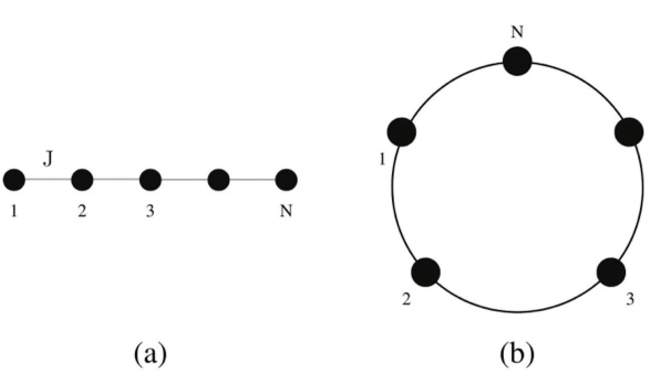
\includegraphics[width=0.7\textwidth]{Immagini/Ising1D_pbc.png}
    \caption{L'immagine (a) è un esempio di modello di Ising 1D senza pbc, mentre in (b) si può apprezzare 
    come la catena si chiuda su se stessa nel caso di condizioni periodiche al contorno. }
    \label{fig: Ising1D_pbc}
\end{figure}

Sebbene il modello di Ising 1D ammetta soluzione esatta, è istruttivo lavorare inizialmente con una teoria di campo 
medio, in cui il termine d'interazione presente nell'Hamiltoniana viene sostituito da un termine efficace (di campo 
medio appunto), andando a trascurare le fluttuazioni degli spin.





\subsection{Teoria di campo medio}

Il punto di partenza di una teoria di campo medio è la semplificazione del temine d'interazione presente nell'Hamiltoniana. Nel  
caso del modello di Ising mono-dimensionale l'interazione fra spin primi vicini può essere riscritta come

\begin{equation}
    \sigma_i \sigma_j\,=\,\left(\sigma_i\,-\,m\,+\,m\right)\left(\sigma_j\,-\,m\,+\,m\right)\,=\,-m^2\,+\,m\sigma_i\,+\,m\sigma_j\,+\,\left(\sigma_i\,-\,m\right)\left(\sigma_j\,-\,m\right),
    \label{eq: int_mf}
\end{equation}

dove l'ultimo termine della somma misura le fluttuazioni fra spin. L'approssimazione di campo medio consiste nel trascurare 
completamente l'ultimo termine, in modo tale che tutti gli spin risultino essere disaccoppiati fra loro e risulti più immediato il 
calcolo della funzione di partizione. L'Hamiltoniana di campo medio risulta quindi 

\begin{equation}
    H_{MF}\,=\,-\frac{J}{2} \sum_{\left<i,j\right>} \left[-m^2\,+\,m\left(\sigma_i\,+\,\sigma_j\right)\right]\,-\,h\sum_{i}\sigma_i,
    \label{eq: ham_mf}
\end{equation}

da cui è immediato il calcolo della funzione di partizione 

\begin{equation}
    Q_{MF}\,=\,\sum_{\left\{\sigma\right\}} e^{-\beta H_{MF}}\,=\,\exp{\left(-\frac{\beta J m^2 N n_{nn}}{2}\right)} \left\{2 \cosh{\left[\beta \left(J n_{nn} m\,+\,h\right)\right]}\right\}^N.
    \label{eq: part_MF_Ising1D}
\end{equation}

Nella relazione precedente la quantità $n_{nn}$ è il numero il numero di coordinazione del reticolo, ossia il numero di primi vicini per la 
geometria presa in considerazione. L'energia libera per particella è data da 

\begin{equation}
    \frac{F}{N}\,=\,-\frac{k_B T}{N} \ln{\left(Q_{MF}\right)}\,=\,\frac{JM^2n_{nn}}{2}\,-\,\frac{1}{\beta}\ln{\left\{2 \cosh{\left[\beta\left(h\,+\,Jn_{nn}m\right)\right]}\right\}}
    \label{eq: freeE_MF_Ising1D}
\end{equation}

da cui è possibile ricavare tutta la termodinamica del sistema.



\subsubsection{Magnetizzazione}

La magnetizzazione si ricava a partire dall'energia libera per spin mediante una derivata rispetto al campo magnetico $h$. 
La relazione che si ottiene è nota come \textit{equazione di Bragg-Williams}, che può essere espressa nella forma 

\begin{equation}
    \tanh^{-1}{\left(m\right)}\,=\,\frac{h\,+\,n_{nn}Jm}{k_B T}
    \label{eq: BW_equation}
\end{equation}

Nel caso in cui il campo magnetico è identicamente nullo, è necessario distinguere due casistiche in base alla temperatura del sistema. 
In primo luogo è necessario introdurre la temperatura critica 

\begin{equation}
    T_c\,=\,\frac{n_{nn}J}{k_B},
    \label{eq: tc_Ising1D_MF}
\end{equation}

che consente di riscrivere il secondo membro dell'equazione di Bragg-Williams in funzione del rapporto fra $T_c$ e la temperatura 
a cui il sistema si trova. Così facendo risulta evidente che quando $T\,>\,T_c$ l'unica soluzione possibile dell'equazione 
\eqref{eq: BW_equation} è $m\,=\,0$, ossia mancanza di magnetizzazione finita. Nel caso opposto, ossia con $T\,<\,T_c$, si hanno 
tre possibili valori di $m$, ossia $0,\,\pm m_0$, con $m_0$ quantità finita. L'energia libera consente di identificare quale 
sia la soluzione fisica, poichè come è possibile osservare in Figura \ref{fig: FE_Ising1D_MF} quando la temperatura scende al 
di sotto di quella critica $F$ passa da un regime in cui è presente un solo minimo in $m\,=\,0$ ad un regime con due minimi 
equivalenti in $m\,=\,\pm m_0\,\neq\,0$. 

\begin{figure}[h!]
    \centering
    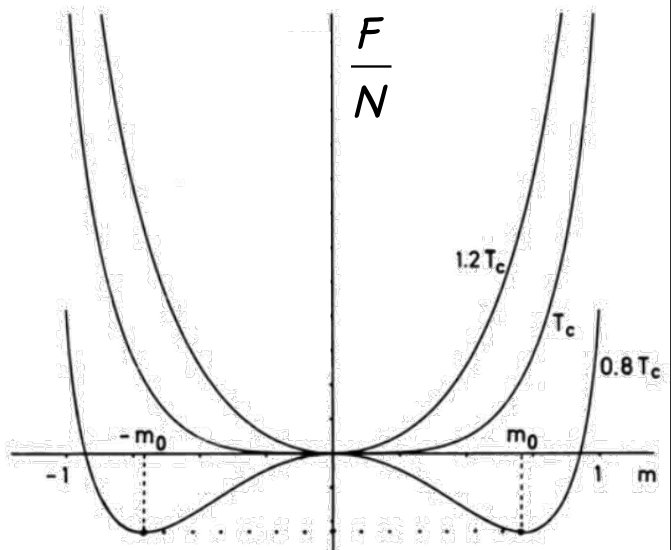
\includegraphics[width=0.7\textwidth]{Immagini/FE_Ising1D_MF.png}
    \caption{ Energia libera per particella al variare della temperatura del sistema. Quando la temperatura è maggiore o uguale 
    di quella critica è presente un solo minimo in $m\,=\,0$, mentre al di sotto sono presenti due minimi globali equivalenti e 
    simmetrici rispetto ad $m\,=\,0$, che è un massimo locale. Immagine da \cite{galliFSA}.}
    \label{fig: FE_Ising1D_MF}
\end{figure}

Questi due valori d'equilibrio della magnetizzazione sono perfettamente simmetrici in assenza di campo magnetico: una 
rottura spontanea della simmetria per inversione di spin è necessaria per far si che il sistema realizzi uno dei due stati di 
minimo globale dell'energia libera. 

Nel caso di campo magnetico esterno diverso da zero non si osserva più la simmetria caratteristica del caso con $h\,=\,0$ e l'
allineamento fra spin concorde con il verso di $h$ risulta essere energeticamente favorito.



\subsubsection{Esponenti critici}

E' possibile caratterizzare il comportamento di un certo sistema nell'intorno del punto critico in termini di leggi di potenza 
che presentano un set di esponenti critici. La seguente analisi è rivolta a 

\begin{table}[h!]
    \centering
    \begin{tabular}{|>{\centering\arraybackslash}p{2cm}|>{\centering\arraybackslash}p{11cm}|}
    \hline
    \textbf{Esponente} & \textbf{Significato fisico} \\ 
    \hline
    $\alpha$ & Descrive l'andamento del calore specifico al punto critico \\ 
    \hline
    $\beta$ & Descrive l'andamento del parametro d'ordine al punto critico \\ 
    \hline
    $\gamma$ & Descrive l'andamento della suscettività al punto critico \\ 
    \hline
    $\delta$ & E' legato all'equazione di stato alla temperatura critica \\ 
    \hline
    \end{tabular}
    \caption{Esponenti critici e relativo significato}
\end{table}

Procediamo ora al calcolo degli esponenti critici $\beta$ e $\delta$ per il modello di Ising mono-dimensionale. L'equazione di Bragg-Williams 
è uno strumento importante per il calcolo di $\beta$, poichè per $T\,\to\,T^-_c$ la magnetizzazione è molto minore di uno ed è possibile 
espandere in serie la tangente iperbolica tralasciando i termini di ordine superiore al terzo 

\begin{equation}
    m\,=\,\tanh{\left(m\frac{T_c}{T}\right)}\,\simeq\,m\frac{T_c}{T}\,-\,\frac{m^3}{3}\left(\frac{T_c}{T}\right)^3
    \label{eq: beta_fp_Ising1D_MF}
\end{equation}

in modo tale che, in seguito ad posto ad uno il fattore moltiplicativo del termine di grado 3, è possibile ricavare la 
magnetizzazione in funzione della differenza fra la temperatura critica e quella a cui si trova il sistema. Dato che 

\begin{equation}
    m\,\simeq\,\sqrt{3\left(\frac{T_c\,-\,T}{T_c}\right)}, 
    \label{eq: beta_sp_Ising1D_MF}
\end{equation}

l'esponente critico $\beta$ sarà pari ad un mezzo. Il calcolo di $\delta$ fa nuovamente uso dell'equazione di Bragg-Williams, che 
a temperature confrontabili con quella critica e per piccoli valori del campo magnetico, può essere espressa come 

\begin{equation}
    m\,=\,\tanh{\left(\frac{h}{k_BT}\,+\,m\frac{T_c}{T}\right)}\,\simeq\,\frac{h}{k_B T}\,+\,m\frac{T_c}{T}\,-\,\frac{1}{3}\left(\frac{h}{k_B T}\,+\,m\frac{T_c}{T}\right)^3
    \label{eq: delta_fp_Ising1D_MF}
\end{equation}

che porta all'equazione di stato approssimata 

\begin{equation}
    \frac{h}{k_B T}\,=\,m\frac{T\,-\,T_c}{T}\,+\,frac{m^3}{3}.
    \label{eq: beta_sp_Ising1D_MF}
\end{equation}

Considerando l'isoterma critica, il primo termine della somma a secondo membro scompare in modo tale che magnetizzazione e 
campo magnetico siano legati come 

\begin{equation}
    m\,\simeq\,\left(\frac{3h}{k_B T_c}\right)^{\frac{1}{3}},
    \label{eq: beta_tp_Ising1D_MF}
\end{equation}

che di conseguenza consente di identificare come $\delta\,=\,3$.





\subsection{Soluzione esatta}

Considerare un sistema con condizioni periodiche al contorno, come (b) in Figura \ref{fig: Ising1D_pbc}, consente 
di scrivere l'Hamiltoniana in forma simmetrica come 

\begin{equation}
    H\,=\,-J\sum_{i} \sigma_i \sigma_{i+1}\,-\,\frac{h}{2}\sum_{i} \left(\sigma_i\,+\,\sigma_{i+1}\right),
    \label{eq: ising_ham_sim}
\end{equation}

dato che $\sigma_{N+1}\,=\,\sigma_1$. La funzione di partizione del sistema è data dalla somma su tutte le possibili 
configurazioni del sistema, che si traduce in 

\begin{equation}
    Q\left(h,\,T\right)\,=\,\sum_{\sigma_1=\pm 1} \cdots \sum_{\sigma_N=\pm 1} \exp{\left\{\beta\left[J\sum_i \sigma_i \sigma_{i+1}\,+\,\frac{h}{2}\sum_i \left(\sigma_i\,+\,\sigma_{i+1}\right)\right]\right\}}
    \label{eq: part_func}
\end{equation}

Definendo una matrice P come

\begin{equation}
    P = \begin{pmatrix}
    e^{\beta\left(J\,+\,h\right)} & e^{-\beta J} \\\\
    e^{-\beta J} & e^{\beta\left(J\,-\,h\right)}
    \end{pmatrix}
    \label{eq: mat_P}
\end{equation}

è possibile riscrivere la funzione di partizione in termini matriciali

\begin{equation}
    Q\left(h,\,T\right)\,=\,\sum_{\sigma_1=\pm 1} \cdots \sum_{\sigma_N=\pm 1} \langle \sigma_1 | P | \sigma_2 \rangle \langle \sigma_2 | P | \sigma_3 \rangle \cdots \langle \sigma_{N-1} | P | \sigma_N \rangle \langle \sigma_N | P | \sigma_1 \rangle 
    \label{eq: part_func_mat}
\end{equation}

Notando che sono presenti $N\,-\,1$ completezze, è possibile procedere ad una semplificazione estrema della relazione 
\eqref{eq: part_func_mat} che consente di apprezzare come la funzione di partizione altro non sia che la traccia della matrice P 
elevata alla N. 

\begin{equation}
    Q\left(h,\,T\right)\,=\,\sum_{\sigma_1=\pm 1} \langle \sigma_1 | P^N | \sigma_1 \rangle \,=\,Tr\left(P^N\right)\,=\,\lambda_1^N\,+\,\lambda_2^N,
    \label{eq: part_func_simp}
\end{equation}

dove $\lambda_1$ e $\lambda_2$ sono gli autovalori della matrice P. La loro determinazione richiede la soluzione di un problema agli 
autovalori, che porta a 

\begin{equation}
    \lambda_{1,2}\,=\,e^{\beta J} \cosh{\left(\beta h\right)}\,\pm\,\sqrt{e^{- 2 \beta J}\,+\,e^{2 \beta J} \sinh^2{\left(\beta h\right)}}.
    \label{eq: autoval_P}
\end{equation}

Una ottima approssimazione, quando il numero di spin preso in considerazione è elevato, consiste nel trascurare il secondo autovalore 
dato che 

\begin{equation}
    \lim_{N \to \infty} \left(\frac{\lambda_2}{\lambda_1}\right)^N\,=\,0.
    \label{eq: approx_Q}
\end{equation}

L'energia libera di Helmholtz, dalla quale è possibile determinare tutta la termodinamica del sistema, risulta quindi

\begin{equation}
    A\left(h,\,T\right)\,=\,-k_B T \ln{\left[Q\left(h,\,T\right)\right]}\,\simeq\,-Nk_BT \ln{\left(\lambda_1\right)}.
    \label{eq: en_lib}
\end{equation}



\subsubsection{Magnetizzazione}

Dall'energia libera di Helmholtz è possibile ricavare la magnetizzazione per spin, che costituisce il parametro d'ordine del 
sistema in analisi ed in quanto tale consente di caratterizzare le transizioni di fase. In particolare, tale quantità si 
ottiene come derivata di $A\left(h,\,T\right)$ rispetto al campo magnetico applicato, in modo tale che

\begin{equation}
    m\,=\,-\left(\frac{\partial A/N}{\partial h}\right)_T\,=\,\frac{\sinh{\left(\beta h\right)}}{\sqrt{e^{-4\beta J}\,+\,\sinh^2\left(\beta h\right)}}
    \label{eq: magn_Ising1D_corr}
\end{equation}

Notiamo che se $h\,\to\,0$ la magnetizzazione tende ad un valore nullo per ogni temperatura finita. Questo fatto evidenzia 
come sia impossibile avere una transizione di fase a temperatura finita T, come invece sembrava evidente nella teoria di campo medio.
Quando si ha $T\,=\,0$ $m$ satura ad uno per ogni valore del campo magnetico, il che implica spin totalmente allineati; questo significa 
che la temperatura critica $T_c$ coincide con lo zero assoluto. E' anche possibile calcolare la suscettività magnetica, la quale diverge 
quanto $T\,\to\,0$, che è il comportamento che ci si aspetterebbe al punto critico. \newline

Il motivo alla base delle errate previsioni della teoria di campo medio è che tale approccio diventa esatto nel limite in cui 
le fluttuazioni del parametro d'ordine sono molto più piccole del valore effettivo dello stesso al punto critico. Il \textit{criterio di Ginzburg} 
afferma che per sistemi tipo Ising, il campo medio fornisce soluzioni esatte solamente per dimensioni del reticolo superiori a 
quattro. Il miglioramento delle previsioni all'aumentare della dimensionalità risulta evidente dal confronto fra gli esponenti 
critici calcolati in campo medio e quelli ottenuti in modo analitico o computazionale mediante simulazioni Monte-Carlo.

\begin{table}[h!]
    \centering
    \begin{tabular}{|>{\centering\arraybackslash}p{3cm}|>{\centering\arraybackslash}p{3cm}|>{\centering\arraybackslash}p{3cm}|>{\centering\arraybackslash}p{3cm}|}  
    \hline
    \textbf{Esponente} & \textbf{Mean-field} & \textbf{Ising 2D} & \textbf{Ising 3D}\\ 
    \hline
    $\alpha$ & 0 & 0 & 0.119 $\pm$ 0.006 \\
    \hline
    $\beta$ & 1/2 & 1/8 & 0.326 $\pm$ 0.004 \\
    \hline
    $\gamma$ & 1 & 7/4 & 1.239 $\pm$ 0.003 \\
    \hline
    $\delta$ & 3 & ? & 4.80 $\pm$ 0.05 \\
    \hline
    $\nu$ & 1/2 & 1 & 0.627 $\pm$ 0.002 \\
    \hline
    \end{tabular}
    \caption{Confronto fra esponenti critici calcolati in campo-medio e in modo analitico/numerico per modelli di Ising 2D e 3D.}
\end{table}



\subsubsection{Correlazioni fra spin}

Consideriamo ora un modello di Ising costituito da un reticolo lineare aperto, senza più condizioni al contorno periodiche, 
come quello in Figura \ref{fig: Ising1D_open}. 

\begin{figure}[H]
    \centering
    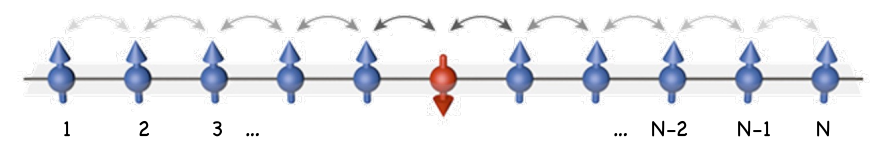
\includegraphics[width=0.7\textwidth]{Immagini/Ising1D_open.png}
    \caption{Esempio di catena di spin per la determinazione della funzione di correlazione fra due spin. Immagine da \cite{galliFSA}.}
    \label{fig: Ising1D_open}
\end{figure}

La funzione di correlazione fra due spin $\sigma_i$ e $\sigma_j$ è definita come

\begin{equation}
    G_{ij}\,=\,\left<\sigma_i \sigma_j\right>\,-\,\left<\sigma_i\right>\left<\sigma_j\right>
    \label{eq: def_corr_fun_Ising1D}
\end{equation}

e consente di valutare se due spin sono correlati o meno. Nel caso del modello di Ising 1D la funzione di correlazione 
risulta essere

\begin{equation}
    G_{i, i+r}\,=\,\left(\tanh{\beta J}\right)^r.
    \label{eq: Ising1D_cor}
\end{equation}

Dall'equazione \eqref{eq: Ising1D_cor} è possibile determinare quale sia la lunghezza di correlazione esprimendo la 
$G_{i, i+r}$ come una funzione esponenzialmente decadente della separazione $r$ fra gli spin in analisi. 

\begin{equation}
    G_{i, i+r}\,=\,e^{r\left[\ln{\left(\tanh{\beta J}\right)}\right]}\,=\,e^{-r/\xi},
    \label{eq: Ising1D_corr_exp}
\end{equation}

da cui risulta che la lunghezza di correlazione è pari a 

\begin{equation}
    \xi\,=\,-\frac{1}{\ln{\left[\tanh{\left(J/k_B T\right)}\right]}}.
    \label{eq: lungh_corr}
\end{equation}

Notiamo che la lunghezza di correlazione è sempre maggiore o uguale a zero. Inoltre, quando la temperatura tende a zero, 
$\xi$ diverge ad infinito. Il fatto che questo accada solamente a temperatura nulla evidenzia come non si abbia correlazione 
(e di conseguenza ordine) a lungo raggio fra gli spin per ogni $T\,\neq\,0$.





\subsection{Simulazioni Monte-Carlo}

L'obiettivo di questa sezione è l'introduzione di delle tecniche Monte-Carlo che consentano di simulare un modello di Ising mono-dimensionale con 
numero di costituenti finito e che presenti condizioni periodiche al contorno, in modo tale che gli spin posti agli estremi della catena 
interagiscano fra loro come primi vicini. Dato che in questo modo tutti gli spin sono equivalenti fra loro ed il sistema è invariante per 
traslazioni, stiamo in pratica simulando un sistema infinito, con un conseguente netto miglioramento della qualità dei risultati. 
Dopo aver definito una condizione iniziale, che solitamente sono quella a temperatura nulla, con tutti gli spin allineati, oppure 
quella a temperatura infinita caratterizzata da momenti magentici orientati casualmente, il primo passo è quello di generare una 
nuova configurazione tentando di invertire uno spin. La differenza in energia fra lo stato di partenza e quello di arrivo determina 
la probabilità d'accettazione della mossa, dato che per l'\textit{algoritmo di Metropolis} \cite{M(RT)2} si ha che 

\begin{equation}
    A\left(\nu\,|\,\mu\right)\,=\,\text{min}\left[1,\,e^{-\beta\left(E_{\nu}\,-\,E_{\mu}\right)}\right]
    \label{eq: Metropolis_1D}
\end{equation}

Chiaramente se la configurazione $\nu$ ha energia inferiore di quella $\mu$, la mossa viene sempre accettata. In caso contrario, è 
possibile che lo spin non venga invertito ed il nuovo elemento della catena di Markov generata dall'algoritmo di Metropolis è identico 
a quello precedente. In seguito è possibile osservare l'implementazione di tale algoritmo in Nim: lo stesso calcolo viene eseguito 
nuovamente ad ogni iterazione, scegliendo lo spin di cui provare il flip in modo casuale.



\subsubsection{Generatore di numeri casuali}

Dato che i metodi Monte-Carlo sono una classe di algoritmi numerici che sfruttano i numeri pseudo-casuali, è auspicabile lavorare 
con un generatore dotato di un lungo periodo (i numeri generati non si ripetono spesso) e che sia efficiente, in modo da ridurre le 
tempistiche computazionali. Le simulazioni che hanno portato ai risultati presenti in questa dispensa sono state effettuate con un 
generatore della famiglia PCG \cite{pcg2014}, di cui è riportata l'implementazione



\begin{minted}[frame=lines, fontsize=\small, bgcolor=blue!10]{nim}
type 
    PCG* = tuple[state, incr: uint64] ##\
    ## The `PCG` type represents the state of a Permuted Congruential 
    ## Generator (PCG), a family of simple fast space-efficient statistically 
    ## good algorithms for random number generation.

    RandomSetUp* = tuple[inState, inSeq: uint64] ##\
    ## The `RandomSetUp` type is used to initialize a `PCG` generator.


proc random*(gen: var PCG): uint64 =
    ## Get a random uint64 from a `PCG`.

    var 
        oldstate = gen.state
        xorshift = uint32(((oldstate shr 18) xor oldstate) shr 27)
        rot = int32(oldstate shr 59)

    gen.state = oldstate * uint64(6364136223846793005) + gen.incr
    result = ((xorshift shr rot) or (xorshift shl ((-rot) and 31)))


proc newRandomSetUp*(rg: var PCG): RandomSetUp {.inline.} = 
    ## Create a new `RandomSetUp` from a `PCG`.
    (rg.random, rg.random)


proc newPCG*(setUp: RandomSetUp): PCG = 
    ## Create a new `PCG` with the given `RandomSetUp`.

    (result.state, result.incr) = (0.uint64, (setUp.inSeq shl 1) or 1)
    discard result.random
    result.state += setUp.inState
    discard result.random


proc rand*(pcg: var PCG): float32 =
    ## Get a random float32 uniformly distributed over the interval (0, 1)
    pcg.random.float32 / 0xffffffff.float32

proc rand*(pcg: var PCG; a, b: float32): float32 =
    ## Get a random float32 uniformly distributed over the interval (a, b)
    a + pcg.rand * (b - a)
\end{minted}    

I numeri pseudo-casuali vengono generati lavorando con interi senza segno, che consentono di fare operazioni fra bit molto efficienti. 
La corretta implementazione è stata testata imponendo un particolare RandomSetUp e valutando la sequenza generata. Sebbene l'implementazione 
del PCG sia riportata nella sezione relativa al modello di Ising mono-dimensionale, tale algoritmo è stato utilizzato anche per l'Ising 2D.



\subsubsection{Termalizzazione}

Una simulazione Monte-Carlo è detta all'equilibrio nel momento in cui viene correttamente campionato il peso statistico di Boltzmann 
$p\left(\mu\right)$. Se il sistema viene inizializzato in uno dei due stati presentati in precedenza, ossia quello a temperatura 
nulla (con spin paralleli) oppure a $T$ infinita (con spin orientati casualmente up oppure down) e si vuole performare una simulazione a 
temperatura finita, sarà necessario del tempo computazionale prima che venga raggiunto l'equilibrio, poichè sara necessario accettare 
alcune mosse.

Un modo qualitativo per valutare la durata della termalizzazione consiste nel graficare una quantità d'interesse, 
come può essere la magnetizzazione oppure l'energia interna del sistema. Tali osservabili presenteranno una fase di transitorio 
iniziale in cui il sistema si scorrela dalla condizione iniziale, per poi fluttuare attorno ad un valore pressochè costante. Non è 
sempre garantito che si raggiunga l'equilibrio, in quanto è possibile rimanere bloccati in uno stato metastabile per tempistiche 
computazionali relativamente lunghe. Per evitare di valutare in maniera errata la durata della fase di termalizzazione è consigliabile 
eseguire lo stesso processo per diverse condizioni iniziali e per diversi seed del generatore di numeri casuali, in modo da considerare 
diverse traiettorie nello spazio delle fasi.  




\subsubsection{Misure e Data-Blocking}

Una volta che il sistema ha raggiunto l'equilibrio, è possibile misurare le osservabili d'interesse senza che i valori d'aspettazione 
siano influenzati dalla fase di transitorio. Per valutare la durata minima della simulazione che consenta di ottenere delle stime 
statisticamente significative è necessaria una misura del tempo di correlazione $t_c$, che esplicita quale sia il numero di mosse 
da effettuare per passare fa uno stato ad un secondo significativamente differente da quello di partenza. Il modo migliore per 
calcolare $t_c$ consiste nello sfruttare la funzione di autocorrelazione temporale, definita per la magnetizzazione come 

\begin{equation}
    \chi\left(t\right)\,=\,\frac{\left<m\left(t'\right)m\left(t'\,+\,t\right)\right>_{t'}\,-\,\left<m\right>^2}{\sigma^2_m}
    \label{eq: auto_corr_m}
\end{equation}

L'autocorrelazione solitamente presenta una caduta esponenziale con tempo caratteristico pari a quello di correlazione

\begin{equation}
    \chi\left(t\right)\,\sim\,e^{-t/t_c}.
    \label{eq: auto_corr_cad_exp}
\end{equation}

Se si considerano due campioni presi ad un $t_c$ di distanza, la funzione di autocorrelazione assume in presenza di un tale 
intervallo temporale un valore di $1/e$, ancora particolarmente significativo. Se si vuole lavorare con quantità realmente indipendenti 
è necessario campionare a $t\,>\,t_c$; solitamente si impone $t\,=\,t_c$ in modo che il numero di misure significative in una 
simulazione di durata $t_{max}$ è pari a 

\begin{equation}
    n\,=\,\frac{t_{max}}{2 t_c}.
    \label{eq: num_ind_samp}
\end{equation}

Per evitare bias nel campionamento e per ottenere dei valori d'aspettazione adeguati è possibile utilizzare la tecnica del 
data-blocking. Le misure delle osservabili di interesse effettuate durante la simulazione, a distanze temporali del tempo di correlazione, 
vengono divise in gruppi, per ciascuno dei quali viene calcolato il valor medio. La dispersione di questi valori medi fornisce una 
stima dell'errore associato alla grandezza calcolata. In Figura \ref{fig: data_block_tech} è presentata visivamente la tecnica del data-
blocking. Le quantità $g_i$ sono le medie di ciascun gruppo.

\begin{figure}[H]
    \centering
    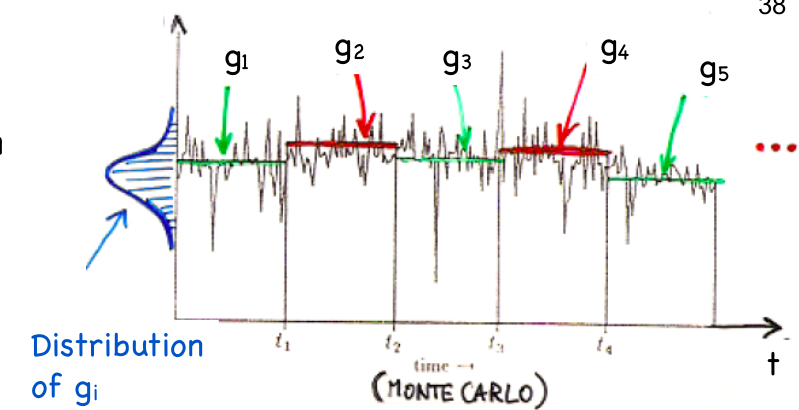
\includegraphics[width=0.6\textwidth]{Immagini/data_blocking.png}
    \caption{Esempio di applicazione della tecnica del data-blocking. Immagine da \cite{galliLSN}.}
    \label{fig: data_block_tech}
\end{figure}

Per determinare quale sia la lunghezza dei blocchi tale da garantire che le medie siano statisticamente indipendenti, si può 
sfruttare il teorema del limite centrale. Nel momento in cui si aumenta la lunghezza dei blocchi, l'errore calcolabile come 

\begin{equation}
    \sigma_{\left<g\right>}\,=\,\sqrt{\frac{1}{N-1}\left(\left<g^2\right>\,-\,\left<g\right>^2\right)}
    \label{eq: error_data_block}
\end{equation}

tende a quello puramente statistico (poichè si va a perdere la correlazione fra le stime) e dopo una certa lunghezza $L$ dei blocchi 
non aumenta più, ma satura ad un valore costante. La lunghezza di saturazione è la minima accettabile per produrre delle stime adeguate. 
Chiaramente maggiore è il numero di blocchi (ossia più lunga è la simulazione), migliore sarà la stima finale della osservabile 
d'interesse.


\newpage
\section{Modello di Ising 2D}

Il modello di Ising 2D è un reticolo quadrato bidimensionale di spin che possono assumere solamente i valori $\pm 1$. L'Hamiltoniana 
del sistema è la stessa riportata in precedenza

\begin{equation}
    H\,=\,-J\sum_{\left<ij\right>} \sigma_i \sigma_j\,-\,h\sum_{i} \sigma_i,
    \label{eq: ising2D_ham}
\end{equation}

con la differenza che in questo caso ogni momento magnetico presenta quattro primi vicini. Il modello presenta soluzione analitica 
solamente nel caso di campo magnetico nullo. In tali condizioni, la magnetizzazione risulta essere 

\begin{equation}
    m\left(\beta,\,h=0\right)\,=\,
    \begin{cases}
    \left[1\,-\,\dfrac{1}{\sinh^4{\left(2\beta J\right)}}\right]^{\frac{1}{8}} \qquad \qquad T\,<\,T_c \\
    0 \qquad \qquad \qquad \qquad \qquad \qquad \,\,\,\, T\,>\,T_c.
    \end{cases}
    \label{eq: magn_Onsager_1944}
\end{equation}

dove $T_c$ è pari a 

\begin{equation}
    T_c\,=\,\frac{2J}{\ln{\left(1\,+\,\sqrt{2}\right)}}.
    \label{eq: tc_Ising2D_Ons}
\end{equation}

Come risulta evidente in Figura \ref{fig: magn_Ising2D}, la magnetizzazione passa rapidamente da un valore unitario a zero nell'intorno 
della temperatura critica. Dato che la magnetizzazione costituisce il parametro d'ordine per il modello di Ising, questo comportamento è
un'evidenza della transizione di fase che il reticolo di spin subisce.

\begin{figure}[H]
    \centering
    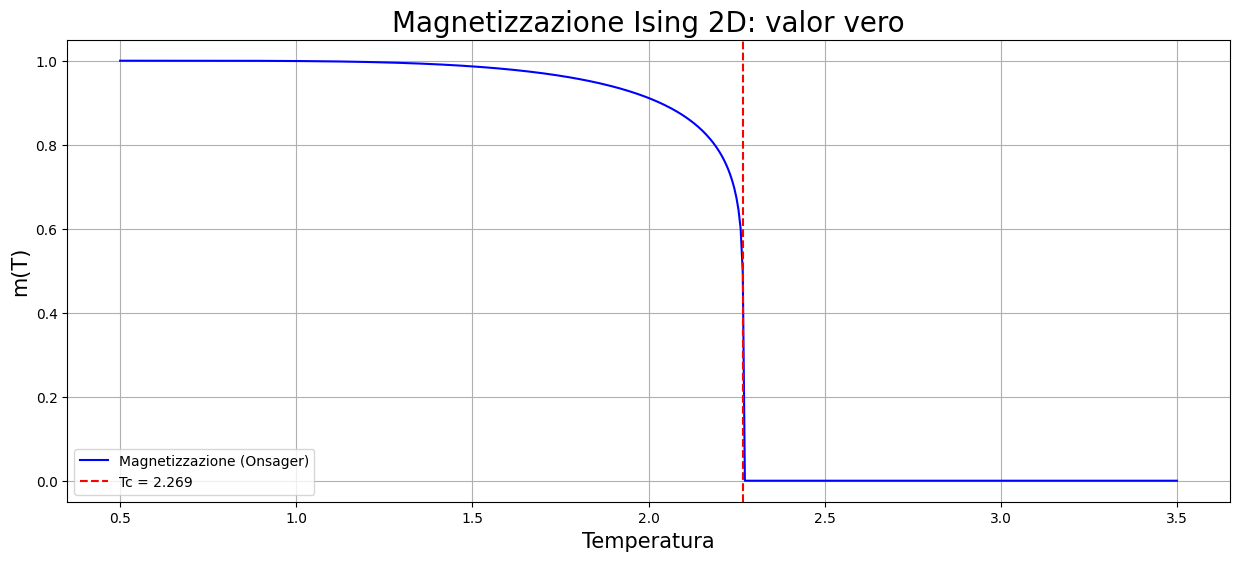
\includegraphics[width=\textwidth]{Immagini/magn_Ising2D.png}
    \caption{Magnetizzazione per il modello di Ising 2D in assenza di campo magnetico. E' possibile osservare come a $T\,=\,T_c$ la 
    magnetizzazione passa rapidamente da un valore unitario a zero. }
    \label{fig: magn_Ising2D}
\end{figure}

Al di sopra della temperatura critica il sistema è di natura paramagnetica e la magnetizzazione è nulla. Invece per $T\,<\,T_c$ gli 
spin sono ordinati ed il sistema presenta magnetizzazione spontanea. Per quanto riguarda l'energia interna, essa 
è data da \cite{Patria}

\begin{equation}
    U\,=\,-NJ\coth{\left(2\beta J\right)}\left\{1\,+\,\frac{2}{\pi}\left[2\tanh^2\left(2\beta J\right)\,-\,1\right]\int_0^{\pi/2}\frac{d\phi}{\sqrt{1\,-\,k^2\sin^2{\left(\phi\right)}}}\right\},
    \label{eq: ene_Onsager_1944}
\end{equation}

dove $k\,=\,2\sinh{\left(2\beta J\right)}/2\cosh^2{\left(2\beta J\right)}$ e l'integrale che compare nella relazione 
precedente è un integrale ellittico completo del primo ordine.



\subsection{Domain walls}

Consideriamo ora un sistema di dimensione lineare $La$, dove $L$ è un numero reale ed $a$ invece il passo reticolare, in uno spazio a $d$ dimensioni. 
Supponiamo inoltre che tale reticolo presenti un domain wall. In analogia con quanto osservato per il modello di Ising 1D, la 
variazione di energia legata a questa struttura è pari a 

\begin{equation}
    \Delta E\,=\,2JL^{d-1}
    \label{eq: ene_dw_IsingdD}
\end{equation}

L'entropia del domain wall è legata al numero di modi in cui si può costruire tale interfaccia. Per un singolo domain wall si può 
stimare che 

\begin{equation}
    S \gtrsim k_B \ln{\left(L\right)}
    \label{eq: entr_dw_IsingdD}
\end{equation}

L'energia libera associata alla presenza dell'interfaccia è dunque pari a 

\begin{equation}
    A \simeq 2JL^{d-1}\,-\,k_B T\ln{\left(L\right)},
    \label{eq: freeE_dw_IsingdD}
\end{equation}

che è dominata dal termine energetico per ogni dimensione maggiore di due, dato che nel limite termodinamico il termine 
logaritmico è trascurabile. Per provare l'esistenza di ferromagnetismo in modo più quantitativo, basta mostrare che il valor medio 
dello spin sia diverso da zero. Nel caso del modello di Ising 2D è possibile mostrare che se gli spin che fanno parte della cornice 
esterna del retico sono positivi, la probabilità di avere uno spin negativo al centro del sistema è pari a 

\begin{equation}
    p_{-}\,<\,\frac{1}{2}\frac{\exp{\left(-2\beta J\right)}}{4 \left(1\,-\,3\exp{\left(-2\beta J\right)}\right)^4}.
    \label{eq: probm_Ising2D}
\end{equation}

Il secondo membro della relazione \eqref{eq: probm_Ising2D} può essere reso minore di $1/2$ in modo indipendente dalla dimensione del reticolo 
(ossia del parametro $L$ introdotto in precedenza) scegliendo una temperatura opportuna. Questo evidenzia come possa 
presentarsi long range order e di conseguenza magnetizzazione finita per $0\,\leq T\,<\,T_c$. Per sottolineare ulteriormente le 
differenze fra il modello di Ising 1D e quello bi-dimensionale consideriamo ora il mapping riportato in Figura \ref{fig: map_2to1_Ising}, 
in cui i siti reticolari di un modello bi-dimensione vengono mappati su una catena lineare (mantendo l'interazione con i primi 
vicini di partenza).

\begin{figure}[H]
    \centering
    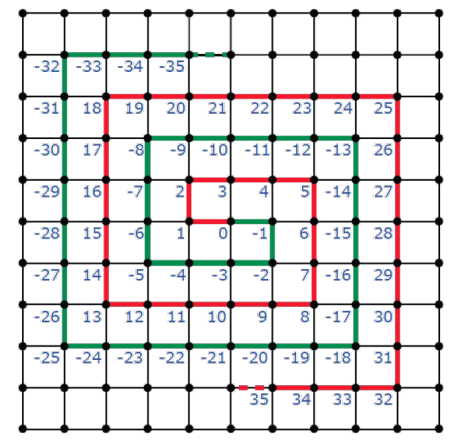
\includegraphics[width=0.35\textwidth]{Immagini/map_2to1_Ising.png}
    \caption{Mapping di un modello di Ising 2D su un modello di Ising 1D. Immagine da \cite{galliFSA}.}
    \label{fig: map_2to1_Ising}
\end{figure}

Sebbene si possa mappare il reticolo quadrato in una catena di spin, il motivo per cui tale reticolo lineare è ordinato a temperatura 
finita è da ricercare nel range dell'interazione. Nel caso del modello di Ising 1D con interazione fra primi vicini, la stessa è short 
range, poichè coinvolge solamente i siti adiacenti a quello preso in considerazione. Nel caso invece di catena di spin ottenuta come 
risultato del mapping di un reticolo quadrato in uno lineare, l'interazione è long-range, ed a ogni nuovo cambio di direzione delle 
spirali concentriche con cui si visitano tutti i siti reticolari tale lunghezza d'interazione aumenta. Nel caso della catena di 
spin ottenuta a partire da un reticolo quadrato anche i domain walls interagiscono fra loro con un potenziale di tipo long-range, andando 
ad invalidare il discorso fatto in precedenza e rendendo possibile una magnetizzazione non nulla anche per una catena di spin. 





\subsection{Fenomeni ad invarianza di scala}

La transizione di fase che avviene alla temperatura critica $T_c$ \eqref{eq: tc_Ising2D_Ons} è una transizione di fase continua. Una delle 
conseguenze della criticità è la perdita di un parametro di scala, nel senso che il sistema presenta cluster di spin di tutte le dimensioni. 
Chiaramente nel caso di una simulazione questa distribuzione sarà influenzata dalle dimensioni finite del reticolo considerato, dato che 
non è computazionalmente possibile lavorare nel limite termodinamico. Inoltre al punto critico il comportamento di un sistema è 
solitamente indipendente dai dettagli microscopici dello stesso, in quanto è determinato da poche caratteristiche quali

\begin{itemize}[label=$\diamond$] 
    \item la dimensionalità $d$ del sistema (per il modello di Ising 2D avremo $d\,=\,2$)
    \item il numero di componenti $n$ del parametro d'ordine
    \item il range delle interazioni microscopiche presenti fra i costituenti del sistema
\end{itemize}

Dato che il comportamento critico del sistema non ha alcuna dipendenza sui gradi di libertà microscopici dello stesso, è possibile mediante 
una tecnica di coarse graining rimuovere i gdL irrilevanti fino a quando si giunge alla lunghezza di correlazione. Tale metodo consiste 
nel dividere il reticolo in blocchi di dimensione inferiore rispetto a quella reticolare e sommare gli spin all'interno dei singoli cluster. 
Se il risultato dell'operazione precedente è positivo, il blocco verrà sostituito da un singolo spin orientato verso l'alto (+1), 
altrimenti da uno che punta verso il basso. Il modello risultante avrà di conseguenza un differente passo reticolare. Bisogna ora  
distinguere tre possibili scenari in base alla temperatura alla quale viene effettuata la simulazione.



\subsubsection{$T\,<\,T_c$}

Al di sotto della temperatura critica, il sistema è dotato di ordine a lungo raggio, ma dato che $T \neq 0$ sono presenti anche cluster 
di grandi dimensioni con spin orientati nella direzione opposta. Applicando in modo iterativo il metodo riportato in precedenza, la 
dimensione della cella unitaria aumenta e le fluttauazioni che sono di dimensione inferiore rispetto al passo reticolare scompaiono. 
Questo implica che il sistema diventa via via più ordinato e tende ad una configurazione con spin totalmente allineati tipica di 
$T\,=\,0$. In Figura \ref{fig: cg_2.0} è riportato un esempio di coarse graining applicato ad un reticolo di $10000 \times 10000$ 
spin, in cui per ogni mossa i sotto-blocchi che vengono presi in considerazione sono di dimensione $10 \times 10$. Si può osservare 
che applicando iterativamente l'algoritmo, le poche eccitazioni presenti nello stato di partenza vengono eliminate, giungendo ad un 
modello con spin completamente allineati. 



\subsubsection{$T\,>\,T_c$}

Al di sopra della temperatura critica, il sistema è disordinato e gli spin formano randomicamente cluster con orientazione verso 
l'alto oppure verso il basso. Ogni volta che viene effettuata una trasformazione, la lunghezza di correlazione diminuisce e i cluster 
diventano di dimensioni inferiori come se la temperatura stesse aumentando. Il sistema tende alla condizione di temperatura infinita, 
con cluster che coinvolgono un numero esiguo di momenti magnetici. In Figura \ref{fig: cg_3.0} è riportato un esempio di coarse graining 
applicato ad un reticolo di $10000 \times 10000$ spin, in cui per ogni mossa i sotto-blocchi che vengono presi in considerazione sono 
di dimensione $10 \times 10$. Si può osservare che applicando iterativamente l'algoritmo il reticolo continua a mantenere le caratteristiche 
tipiche dell'alta temperatura, ossia cluster di spin di piccole dimensioni.



\subsubsection{$T\,=\,T_c$}

Alla temperatura critica, i cluster sono di tutte le dimensioni, partendo da singoli spin per giungere ad un numero macroscopico di 
momenti magnetici coinvolti. In questo caso la lunghezza di correlazione è infinita e per iterazioni successive del metodo introdotto 
in precedenza non si ha alcun cambio nella distrubuzione delle dimensioni dei cluster. Il reticolo rimane a $T_c$, che risulta essere 
un punto fisso della funzione di coarse-graining. Chiaramente, gli altri punti fissi sono $T\,=\,0$ e $T\,=\,\infty$ a cui tendono 
tutti i sistemi che non si trovano in partenza al punto critico.


\vspace*{\fill}

\begin{figure}[htbp]
    \centering
    \begin{minipage}{0.45\textwidth}  
      \centering
      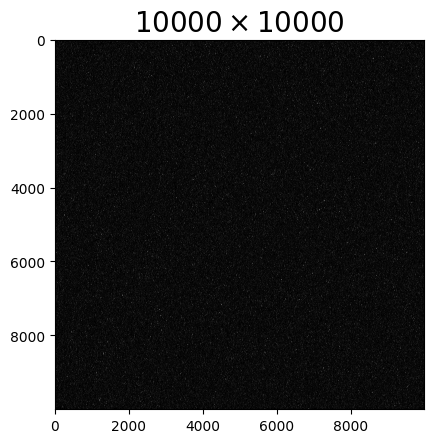
\includegraphics[page=1, width=\textwidth]{Immagini/simIsing2D/cg/cg_10000_2.0.png}
      \caption{Stato iniziale}
    \end{minipage}\hfill
    \begin{minipage}{0.45\textwidth}  
      \centering
      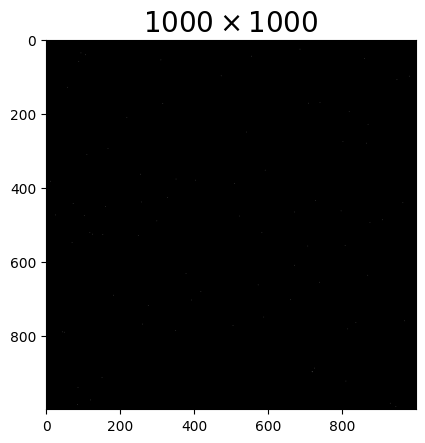
\includegraphics[page=1, width=\textwidth]{Immagini/simIsing2D/cg/cg_1000_2.0.png}
      \caption{Prima iterazione}
    \end{minipage}
    \vskip\baselineskip 
  
    \begin{minipage}{0.45\textwidth}  
      \centering
      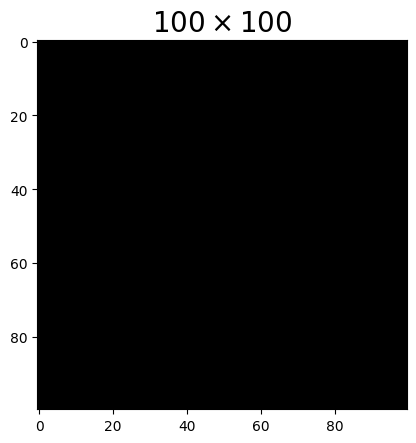
\includegraphics[page=1, width=\textwidth]{Immagini/simIsing2D/cg/cg_100_2.0.png}
      \caption{Seconda iterazione}
    \end{minipage}\hfill
    \begin{minipage}{0.45\textwidth}  
      \centering
      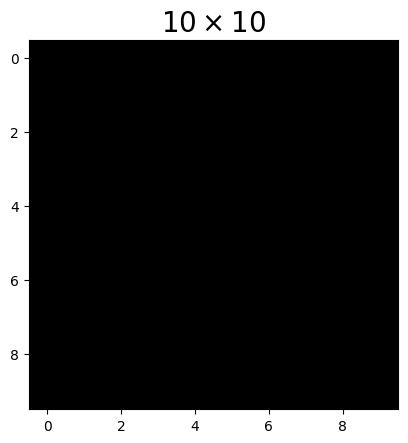
\includegraphics[page=1, width=\textwidth]{Immagini/simIsing2D/cg/cg_10_2.0.png}
      \caption{Terza iterazione}
    \end{minipage}

    \caption{Esempio di coarse-graining per un reticolo di $10000 \times 10000$ spin in equilibrio termodinamico alla 
    temperatura $T\,=\,2.0$. Ogni iterazione dell'algoritmo riduce di un fattore 10 il numero degli spin costituenti i lati 
    del quadrato.}
    \label{fig: cg_2.0}
\end{figure}

\vspace*{\fill}

\vspace*{\fill}

\begin{figure}[htbp]
    \centering
    \begin{minipage}{0.45\textwidth}  
      \centering
      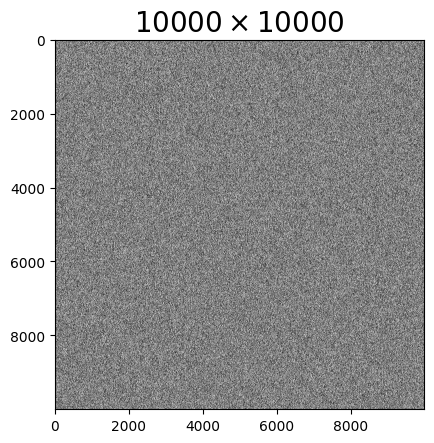
\includegraphics[page=1, width=\textwidth]{Immagini/simIsing2D/cg/cg_10000_3.0.png}
      \caption{Stato iniziale}
    \end{minipage}\hfill
    \begin{minipage}{0.45\textwidth}  
      \centering
      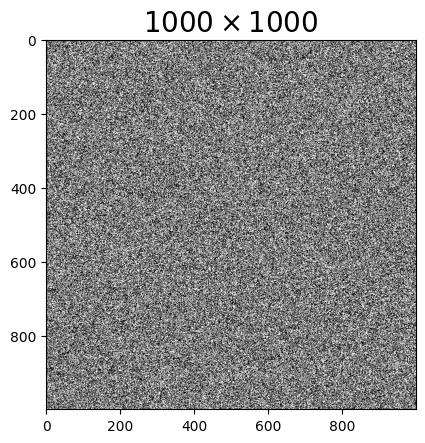
\includegraphics[page=1, width=\textwidth]{Immagini/simIsing2D/cg/cg_1000_3.0.png}
      \caption{Prima iterazione}
    \end{minipage}
    \vskip\baselineskip 
  
    \begin{minipage}{0.45\textwidth}  
      \centering
      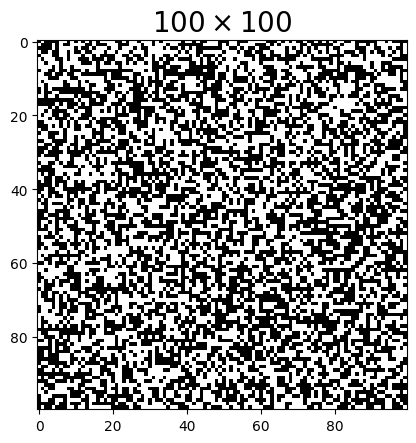
\includegraphics[page=1, width=\textwidth]{Immagini/simIsing2D/cg/cg_100_3.0.png}
      \caption{Seconda iterazione}
    \end{minipage}\hfill
    \begin{minipage}{0.45\textwidth}  
      \centering
      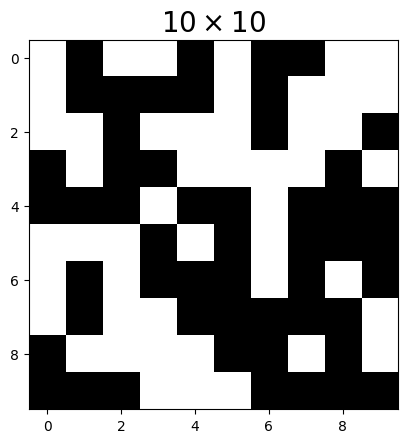
\includegraphics[page=1, width=\textwidth]{Immagini/simIsing2D/cg/cg_10_3.0.png}
      \caption{Terza iterazione}
    \end{minipage}

    \caption{Esempio di coarse-graining per un reticolo di $10000 \times 10000$ spin in equilibrio termodinamico alla 
    temperatura $T\,=\,3.0$. Ogni iterazione dell'algoritmo riduce di un fattore 10 il numero degli spin costituenti i lati 
    del quadrato.}
    \label{fig: cg_3.0}
\end{figure}

\vspace*{\fill}
\newpage
\section{Simulazioni Monte-Carlo}

L'obiettivo di questa sezione è l'introduzione di tecniche Monte-Carlo che consentano di simulare un modello di Ising con 
numero di costituenti finito. I reticoli considerati sono dotati di condizioni periodiche al contorno, in modo tale che gli spin 
posti agli estremi interagiscano fra loro come primi vicini. Dato che in questo modo tutti gli spin sono equivalenti fra loro ed 
il sistema è invariante per traslazioni, stiamo in pratica simulando un sistema infinito, con un conseguente netto miglioramento 
nella qualità dei risultati. 





\subsection{Generatore di numeri casuali}

Dato che i metodi Monte-Carlo sono una classe di algoritmi numerici che si basano sull'utilizzo di numeri pseudo-casuali, è auspicabile lavorare 
con un generatore dotato di un lungo periodo di generazione. Inoltre il generatore deve essere efficiente, in modo da mantenere contenute le 
tempistiche computazionali. Le simulazioni che hanno portato ai risultati presenti in questa dispensa sono state effettuate con un 
generatore della famiglia PCG \cite{pcg2014}, di cui è riportata l'implementazione. Il linguaggio utilizzato è il Nim, che compila 
direttamente in codice macchina (alte prestazioni), ma presenta una sintassi molto semplice, che ricorda quella del Python.


\begin{minted}[frame=lines, fontsize=\small, bgcolor=blue!10, breaklines = true]{nim}
type 
    PCG* = tuple[state, incr: uint64] ##\
    ## The `PCG` type represents the state of a Permuted Congruential 
    ## Generator (PCG), a family of simple fast space-efficient statistically 
    ## good algorithms for random number generation.

    RandomSetUp* = tuple[inState, inSeq: uint64] ##\
    ## The `RandomSetUp` type is used to initialize a `PCG` generator.


proc random*(gen: var PCG): uint64 =
    ## Get a random uint64 from a `PCG`.

    var 
        oldstate = gen.state
        xorshift = uint32(((oldstate shr 18) xor oldstate) shr 27)
        rot = int32(oldstate shr 59)

    gen.state = oldstate * uint64(6364136223846793005) + gen.incr
    result = ((xorshift shr rot) or (xorshift shl ((-rot) and 31)))


proc newRandomSetUp*(rg: var PCG): RandomSetUp {.inline.} = 
    ## Create a new `RandomSetUp` from a `PCG`.
    (rg.random, rg.random)


proc newPCG*(setUp: RandomSetUp): PCG = 
    ## Create a new `PCG` with the given `RandomSetUp`.

    (result.state, result.incr) = (0.uint64, (setUp.inSeq shl 1) or 1)
    discard result.random
    result.state += setUp.inState
    discard result.random


proc rand*(pcg: var PCG): float32 =
    ## Get a random float32 uniformly distributed over the interval (0, 1)
    pcg.random.float32 / 0xffffffff.float32

proc rand*(pcg: var PCG; a, b: float32): float32 =
    ## Get a random float32 uniformly distributed over the interval (a, b)
    a + pcg.rand * (b - a)
\end{minted}    

I numeri pseudo-casuali vengono generati lavorando con interi senza segno, che consentono di fare operazioni fra bit molto efficienti. 
La corretta implementazione è stata testata imponendo un particolare RandomSetUp e valutando la sequenza generata. 





\subsection{Inizializzazione}

Il primo step della simulazione consiste nel definire una condizione iniziale. Solitamente le scelte più comuni sono la configurazione 
a temperatura nulla (con tutti gli spin allineati) oppure quella a temperatura infinita (con momenti magnetici orientati casualmente). 
Chiaramente tale condizione iniziale non è all'equilibrio per la temperatura alla quale si vuole simulare il sistema. Sarà necessaria 
una fase di termalizzazione in cui il reticolo si rilassa fino a giungere all'equilibrio termodinamico, dopo la quale sarà poi possibile 
iniziare a misurare le osservabili di nostro interesse. Per procedere nello studio del modello è quindi necessario introdurre dei metodi 
che consentano di generare una nuova configurazione e quindi di evolvere il sistema. Le simulazioni riportate in questa dispensa 
hanno fatto uso dell'\textit{algoritmo di Metropolis} e dell'\textit{algoritmo di Wolff}.





\subsection{Algoritmo di Metropolis}

Una mossa dell'algoritmo di Metropolis consiste nel selezionare casualmente uno spin del reticolo con l'obiettivo di generare una 
nuova configurazione invertendolo. La differenza in energia fra lo stato di partenza e quello di arrivo determina 
la probabilità d'accettazione della mossa, dato che per l'\textit{algoritmo di Metropolis} \cite{M(RT)2} si ha che 

\begin{equation}
    A\left(\nu\,|\,\mu\right)\,=\,\text{min}\left[1,\,e^{-\beta\left(E_{\nu}\,-\,E_{\mu}\right)}\right]
    \label{eq: Metropolis_1D}
\end{equation}

Chiaramente se la configurazione $\nu$ ha energia inferiore di quella $\mu$, la mossa viene sempre accettata. In caso contrario, è 
possibile che lo spin non venga invertito e che il nuovo elemento della catena di Markov generata dall'algoritmo di Metropolis sia identico 
a quello precedente. Eseguire $N_{spin}$ volte il ciclo precedente, ossia tentare in media un'inversione per spin, equivale ad aver 
completato uno \textit{sweep} del reticolo. Per le successive fasi conviene studiare le osservabili del sistema in funzione degli sweep e 
non delle singole mosse dell'algoritmo di Metropolis: per questo motivo le implementazioni dell'algoritmo riportato in seguito 
eseguono uno sweep a chiamata, ossia tentano ogni volta $N_{spin}$ inversione. Anche in questo caso il codice riportato è in Nim.



\subsubsection{Metropolis Ising 1D}

\begin{minted}[frame=lines, fontsize=\small, bgcolor=blue!10, breaklines = true]{nim}
    proc metropolisMove*(modIsing: var seq[int], rg: var PCG, temp: float32, acc: float32, hmagn: float32, accettate: var int) = 
    # Algoritmo di Metropolis per evolvere il modello di Ising

    # Indice per selezionare lo spin
    var 
        diffE: float32
        ind, prev, next, appo: int


    for i in 0..<len(modIsing):
        ind = int(rg.rand(float32(0), float32(len(modIsing)))) mod len(modIsing)
        prev = if (ind - 1) mod len(modIsing) == -1: len(modIsing)-1 else: (ind - 1) mod len(modIsing)
        next = (ind + 1) mod len(modIsing)

        appo = modIsing[ind]
        diffE = 2 * acc * float32(appo) * float32(modIsing[prev] + modIsing[next]) + 2 * hmagn * float32(appo)

        if diffE < 0:
            modIsing[ind] = -appo
            accettate += 1

        elif rg.rand() < exp(-diffE/temp):
            modIsing[ind] = -appo
            accettate += 1
\end{minted}    



\subsubsection{Metropolis Ising 2D}

\begin{minted}[frame=lines, fontsize=\small, bgcolor=blue!10, breaklines = true]{nim}
    proc metropolisMove*(modIsing: var seq[seq[int]], rg: var PCG, temp: float32, acc: float32, nspin: int, accettate: var int) = 
    # Algoritmo di Metropolis per evolvere il modello di Ising 2D

    # Indice per selezionare lo spin
    var 
        nmove = int(nspin * nspin)
        diffE: float32
        xcoor, ycoor, appo: int
        up, down, left, right: int


    for i in 0..<nmove:

        # Seleziono casualmente uno spin facente parte del modello
        xcoor = int(floor(rg.rand(float32(0), float32(nspin)))) mod nspin
        ycoor = int(floor(rg.rand(float32(0), float32(nspin)))) mod nspin

        # Determino quali sono i primi vicini in questo caso (facendo attenzione a bc)
        down = (ycoor + 1) mod nspin
        right = (xcoor + 1) mod nspin
        up = (ycoor - 1 + nspin) mod nspin
        left = (xcoor - 1 + nspin) mod nspin

        # Calcolo i contributi energetici
        appo = modIsing[xcoor][ycoor]
        diffE = 2 * acc * float32(appo) * float32((modIsing[right][ycoor] + modIsing[left][ycoor] + modIsing[xcoor][up] + modIsing[xcoor][down]))

        if diffE < 0:
            modIsing[xcoor][ycoor] = -appo
            accettate += 1

        elif rg.rand() < exp(-diffE/temp):
            modIsing[xcoor][ycoor] = -appo
            accettate += 1
\end{minted}    

L'unica differenza fra le due implementazioni riportate in precedenza è la gestione delle condizioni al 
contorno, chiaramente più complessa in due dimensioni dato che il numero di primi vicini duplica, passando 
da due a quattro. La struttura in sè dell'algoritmo rimane la stessa. 





\subsection{Termalizzazione}

Una simulazione Monte-Carlo è detta all'equilibrio nel momento in cui viene correttamente campionato il peso statistico di Boltzmann 
$p\left(\mu\right)$. Se il sistema viene inizializzato in uno dei due stati presentati in precedenza, ossia quello a temperatura 
nulla (con spin paralleli) oppure a $T$ infinita (con spin orientati casualmente up oppure down) e si vuole performare una simulazione a 
temperatura finita, sarà necessario del tempo computazionale prima che venga raggiunto l'equilibrio, poichè sara necessario accettare 
alcune mosse.

Un modo qualitativo per valutare la durata della termalizzazione consiste nel graficare una quantità d'interesse, 
come può essere la magnetizzazione oppure l'energia interna del sistema. Tali osservabili presenteranno una fase di transitorio 
iniziale in cui il sistema si scorrela dalla condizione iniziale, per poi fluttuare attorno ad un valore pressochè costante. Non è 
sempre garantito che si raggiunga l'equilibrio, in quanto è possibile rimanere bloccati in uno stato metastabile per tempistiche 
computazionali relativamente lunghe. Per evitare di valutare in maniera errata la durata della fase di termalizzazione è consigliabile 
eseguire lo stesso processo per diverse condizioni iniziali e per diversi seed del generatore di numeri casuali, in modo da considerare 
diverse traiettorie nello spazio delle fasi. In Figura \ref{fig: term_Ising1D} è riportato la termalizzazione di un modello di Ising 
1D da 3000 spin a temperatura $T\,=\,0.5$: in questo caso dopo circa 500 sweep della catena viene raggiunto l'equilibrio termodinamico.

\begin{figure}[H]
    \centering
    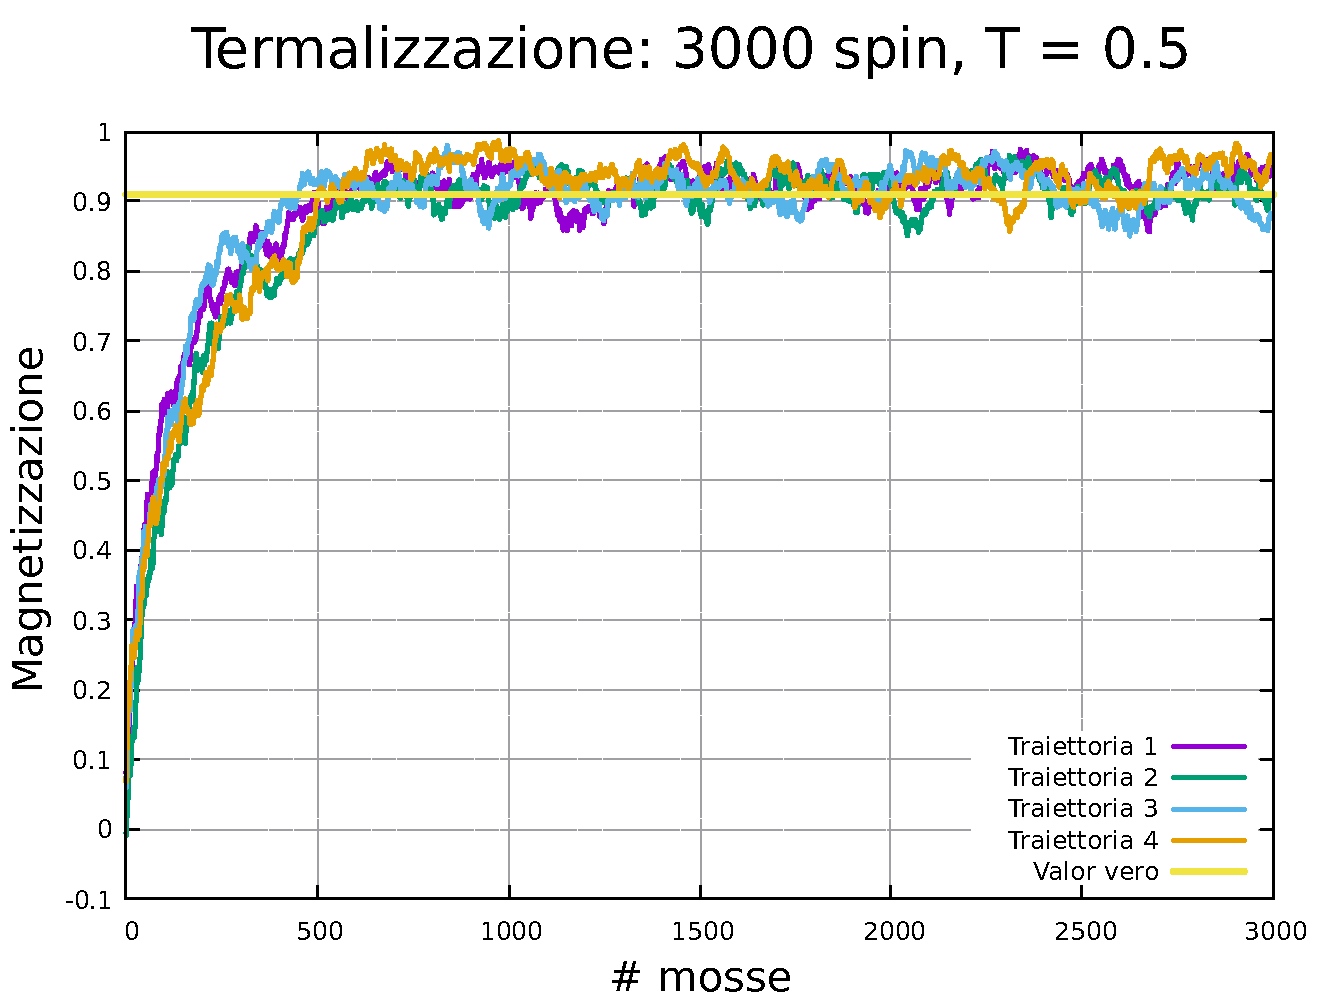
\includegraphics[width=0.6\textwidth]{Immagini/MC_meth/term_3000_0.5.pdf}
    \caption{Termalizzazione per un modello di Ising 1D da 3000 spin a temperatura $T\,=\,0.5$}
    \label{fig: data_block_tech}
\end{figure}



\subsection{Autocorrelazione}

Una volta che il sistema ha raggiunto l'equilibrio, è possibile misurare le osservabili d'interesse senza che i valori d'aspettazione 
siano influenzati dalla fase di transitorio. Per valutare la durata minima della simulazione che consenta di ottenere delle stime 
statisticamente significative è necessaria una misura del tempo di correlazione $t_c$, che esplicita quale sia il numero di sweep 
da effettuare per passare da uno stato ad un altro significativamente differente da quello di partenza. Il modo migliore per 
calcolare $t_c$ consiste nello sfruttare la funzione di autocorrelazione temporale, definita per la magnetizzazione come 

\begin{equation}
    \chi\left(t\right)\,=\,\frac{\left<m\left(t'\right)m\left(t'\,+\,t\right)\right>_{t'}\,-\,\left<m\right>^2}{\sigma^2_m}
    \label{eq: auto_corr_m}
\end{equation}

L'autocorrelazione solitamente presenta una caduta esponenziale con tempo caratteristico pari a quello di correlazione

\begin{equation}
    \chi\left(t\right)\,\sim\,e^{-t/t_c}.
    \label{eq: auto_corr_cad_exp}
\end{equation}

Se si considerano due campioni presi ad un $t_c$ di distanza, la funzione di autocorrelazione assume in presenza di un tale 
intervallo temporale un valore di $1/e$, ancora particolarmente significativo. Se si vuole lavorare con quantità realmente indipendenti 
è necessario campionare a $t\,>\,t_c$; solitamente si impone $t\,=\,2t_c$ in modo che il numero di misure significative in una 
simulazione di durata $t_{max}$ sia pari a 

\begin{equation}
    n\,=\,\frac{t_{max}}{2 t_c}.
    \label{eq: num_ind_samp}
\end{equation}

In Figura \ref{fig: autocorr_Ising_ex} è riportato un esempio di calcolo della funzione di autocorrelazione per un reticolo di spin 
$500 \times 500$ a temperatura pari a due. In questo caso specifico i valori della magnetizzazione sono scorrelati dopo circa 50 sweeps.

\begin{figure}[H]
    \centering
    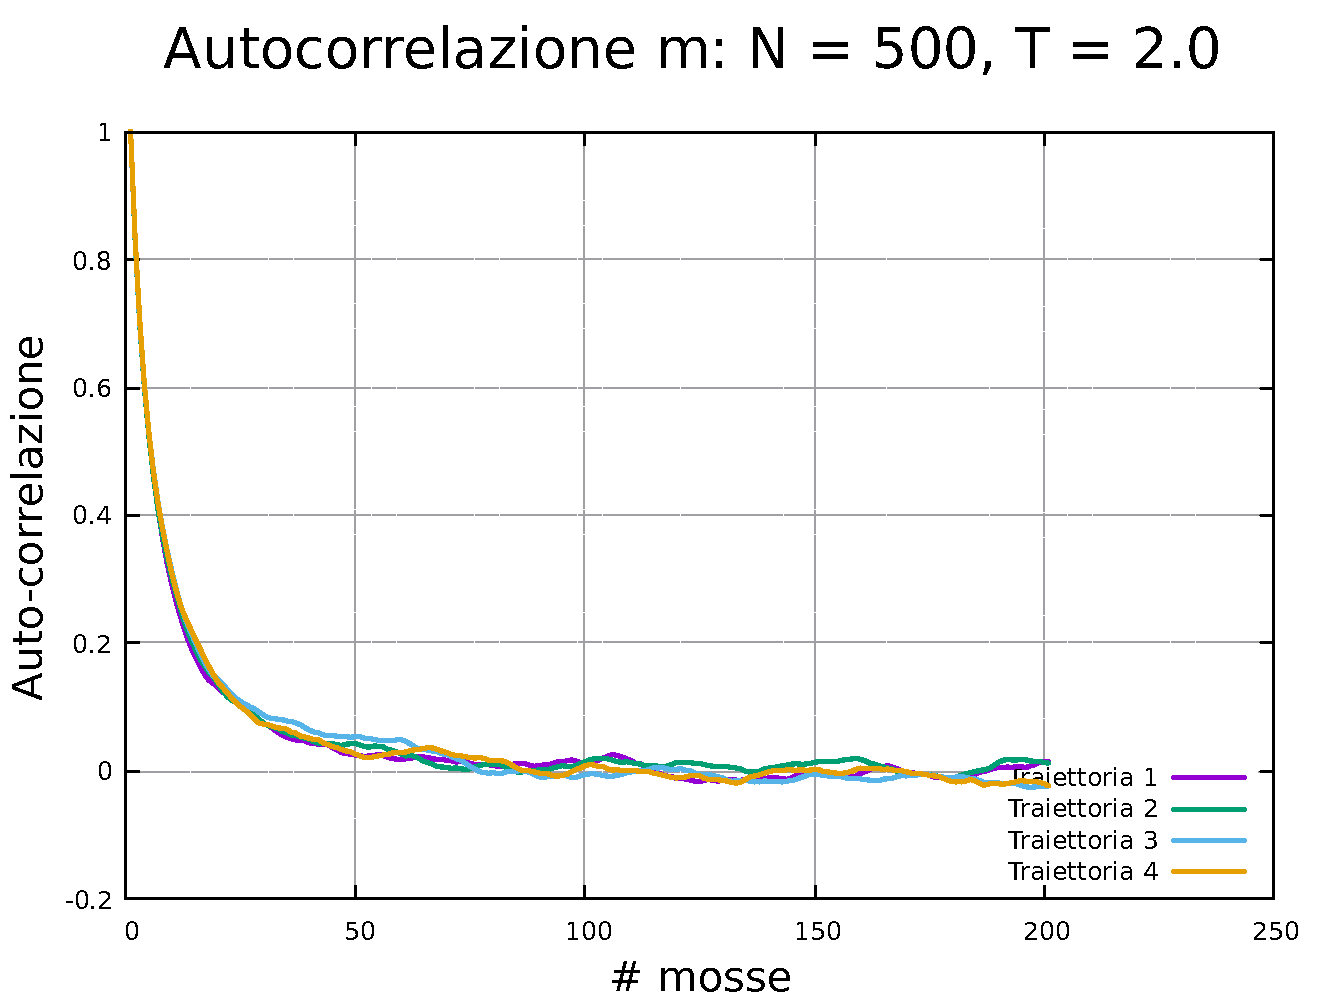
\includegraphics[width=0.6\textwidth]{Immagini/MC_meth/auto_500_2.0.pdf}
    \caption{Autocorrelazione per un modello di Ising 2D di dimensione $500 \times 500$ a temperatura $T\,=\,2.0$}
    \label{fig: autocorr_Ising_ex}
\end{figure}



\subsection{Data-blocking}

Per evitare bias nel campionamento e per ottenere dei valori d'aspettazione adeguati è possibile utilizzare la tecnica del 
data-blocking. Le misure delle osservabili di interesse effettuate durante la simulazione, a distanze temporali inferiori del tempo di correlazione, 
vengono divise in gruppi, per ciascuno dei quali viene calcolato il valor medio. La dispersione di questi valori medi fornisce una 
stima dell'errore associato alla grandezza calcolata. In Figura \ref{fig: data_block_tech} è presentata visivamente la tecnica del 
data-blocking. Le quantità $g_i$ sono le medie di ciascun gruppo.

\begin{figure}[H]
    \centering
    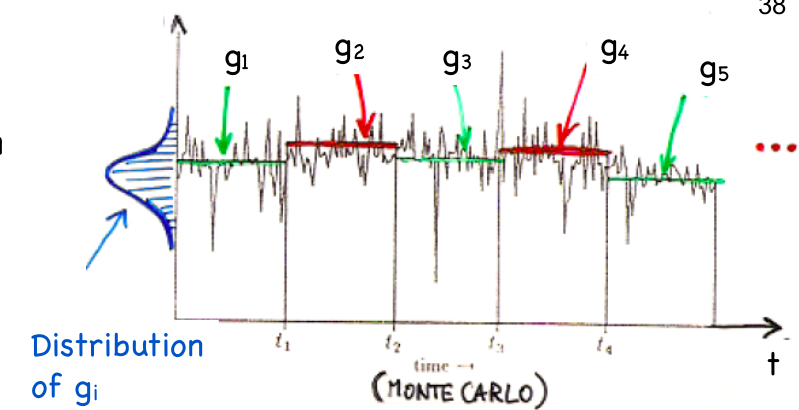
\includegraphics[width=0.6\textwidth]{Immagini/data_blocking.png}
    \caption{Esempio di applicazione della tecnica del data-blocking. Immagine da \cite{galliLSN}.}
    \label{fig: data_block_tech}
\end{figure}

Per determinare quale sia la lunghezza dei blocchi tale da garantire che le medie siano statisticamente indipendenti, si può 
sfruttare il teorema del limite centrale. Nel momento in cui si aumenta la lunghezza dei blocchi, l'errore calcolabile come 

\begin{equation}
    \sigma_{\left<g\right>}\,=\,\sqrt{\frac{1}{N-1}\left(\left<g^2\right>\,-\,\left<g\right>^2\right)}
    \label{eq: error_data_block}
\end{equation}

tende a quello puramente statistico (poichè si va a perdere la correlazione fra le stime) ed oltre una certa lunghezza $L$ dei blocchi 
satura ad un valore costante. La lunghezza di saturazione è la minima accettabile per produrre delle stime adeguate. 
Chiaramente maggiore è il numero di blocchi (della corretta dimensione), migliore sarà la stima finale della osservabile 
d'interesse. In Figura \ref{fig: lblk_exe} è riportato un esempio di stima della dimensione dei blocchi per un reticolo di spin 
$500 \times 500$ a temperatura pari a due. In questo caso specifico possiamo lavorare con blocchi di lunghezza 150 sweeps.

\begin{figure}[H]
    \centering
    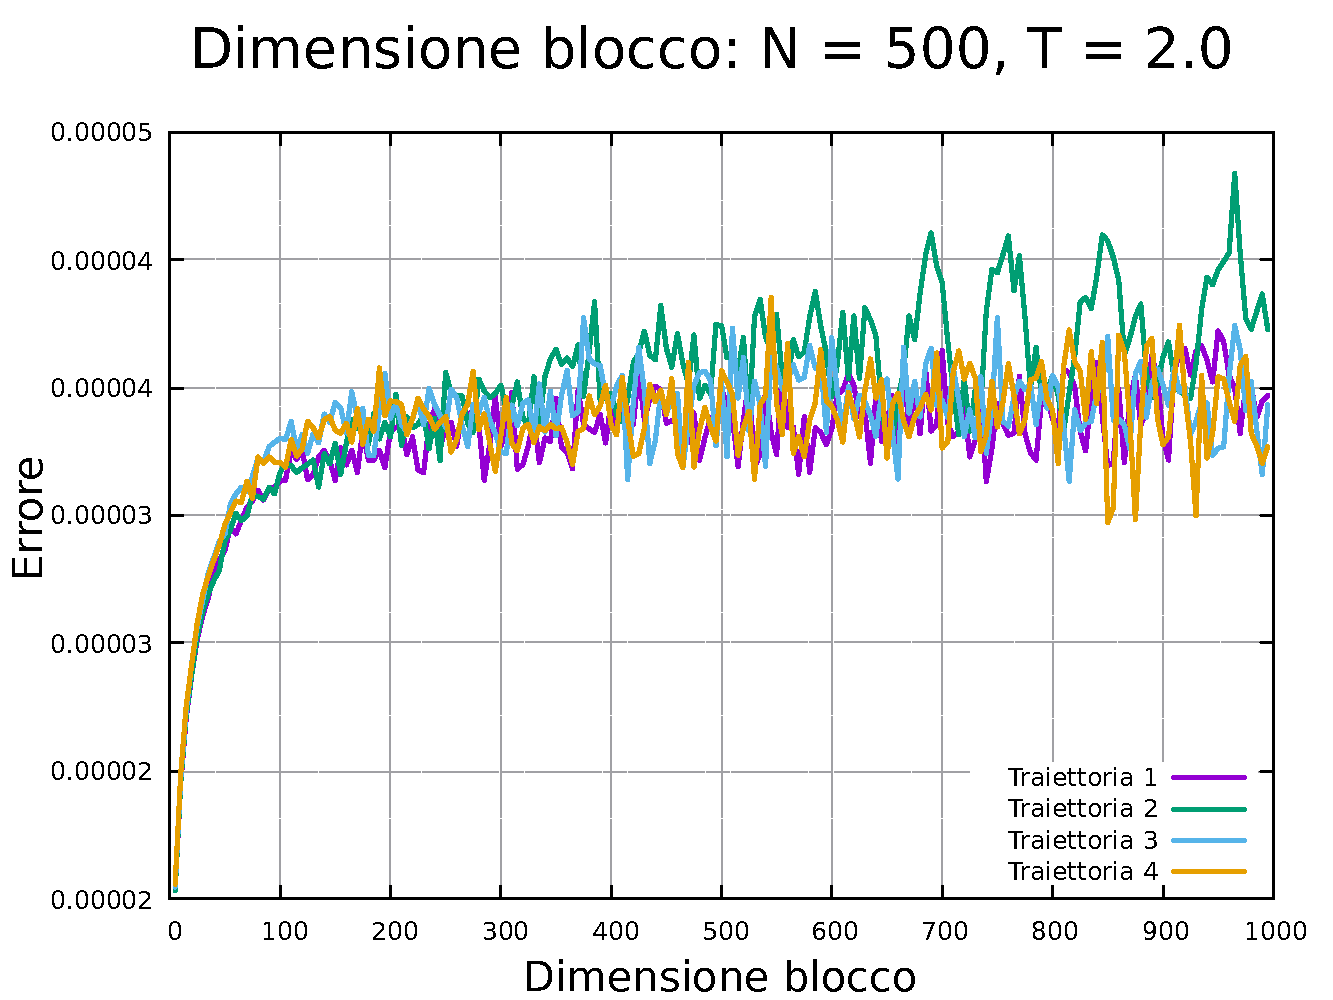
\includegraphics[width=0.6\textwidth]{Immagini/MC_meth/err_500_2.0.pdf}
    \caption{Studio delle dimensioni dei blocchi per un modello di Ising 2D di dimensione $500 \times 500$ a temperatura $T\,=\,2.0$}
    \label{fig: lblk_exe}
\end{figure}





\subsection{Algoritmo di Wolff}

L'algoritmo di Metropolis, anche grazie alla sua semplicità, è il più performante al di fuori della regione 
critica. Tuttavia, quando la temperatura del sistema tende a $T_c$, gli spin tendono a raggrupparsi in 
grandi cluster che contribuiscono significativamente alla magnetizzazione ed all'energia, e nel momento in 
cui cambia l'orientamento degli spin si producono grandi fluttuazioni, note come \textit{fluttuazioni critiche}. 
Questo aspetto, insito nella natura del modello di Ising, comporta un aumento dell'errore statistico 
associato ai valori d'aspettazione degli osservabili, ma è indipendente dall'algoritmo considerato. Un secondo aspetto è legato 
all'aumento della lunghezza di correlazione $\xi$, che nel limite termodinamico diverge alla temperatura critica. Sappiamo che $\xi$ 
è legato al tempo di correlazione dalla relazione 

\begin{equation}
    \tau \propto \xi^z
    \label{eq: tcorr_lcorr}
\end{equation}

Maggiore è $z$, peggio l'algoritmo riesce a generare configurazioni indipendenti fra loro. Per Metropolis, il valore universalmente 
riconosciuto per l'esponente è $z\,=\,2.1665 \pm 0.0012$, che è piuttosto alto \cite{MCM}. Al punto critico, l'algoritmo di Metropolis è vittima 
di \textit{critical slowing down}, dovuto al fatto che è un algoritmo locale (tenta di invertire uno spin alla volta) e quindi non 
riesce a far fronte all'aumento incontrollato della lunghezza di correlazione. Un modo per cercare di ridurre il valore di $z$ è quello 
di lavorare su cluster di spin, in modo tale da invertire contemporaneamente un numero maggiore di spin. L'algoritmo di Wolff, che nelle 
simulazioni qui riportate è stato utilizzato per studiare il punto critico del modello di Ising 2D, sfrutta questa idea e per questo 
motivo fa parte della famiglia degli \textit{algoritmi di clustering}. Uno dei punti cruciali dell'algoritmo consiste nell'identificazione 
del cluster di spin da invertire. La dimensione del blocco dovrebbe dipendere dalla temperatura a cui stiamo simulando il modello, perchè 
per esempio per $T \gg T_c$ gli spin tendono ad essere fra loro scorrelati, evidenziando come dovrebbero essere considerati solo pochi 
momenti magnetici alla volta. L'opposto si può dire del caso a bassa temperatura. Per questo motivo nel momento in cui due spin adiacenti 
hanno lo stesso orientamento non è automatico che essi appartengano allo stesso cluster, ma è presente una certa probabilità di aggiunta 
che aumenta al diminuire della temperatura. Nel caso dell'algoritmo di Wolff, tale probabilità è pari a 

\begin{equation}
    P_{add}\,=\,1\,-\,\exp{\left(-2\beta J\right)}
    \label{eq: padd_cluster}
\end{equation}

In Figura \ref{fig: dim_clW} è riportata la frazione di reticolo ricoperta dal cluster in funzione della temperatura. La probabilità 
introdotta in \eqref{eq: padd_cluster} garantisce la dipendenza corretta al variare della temperatura del modello.

\begin{figure}[H]
    \centering
    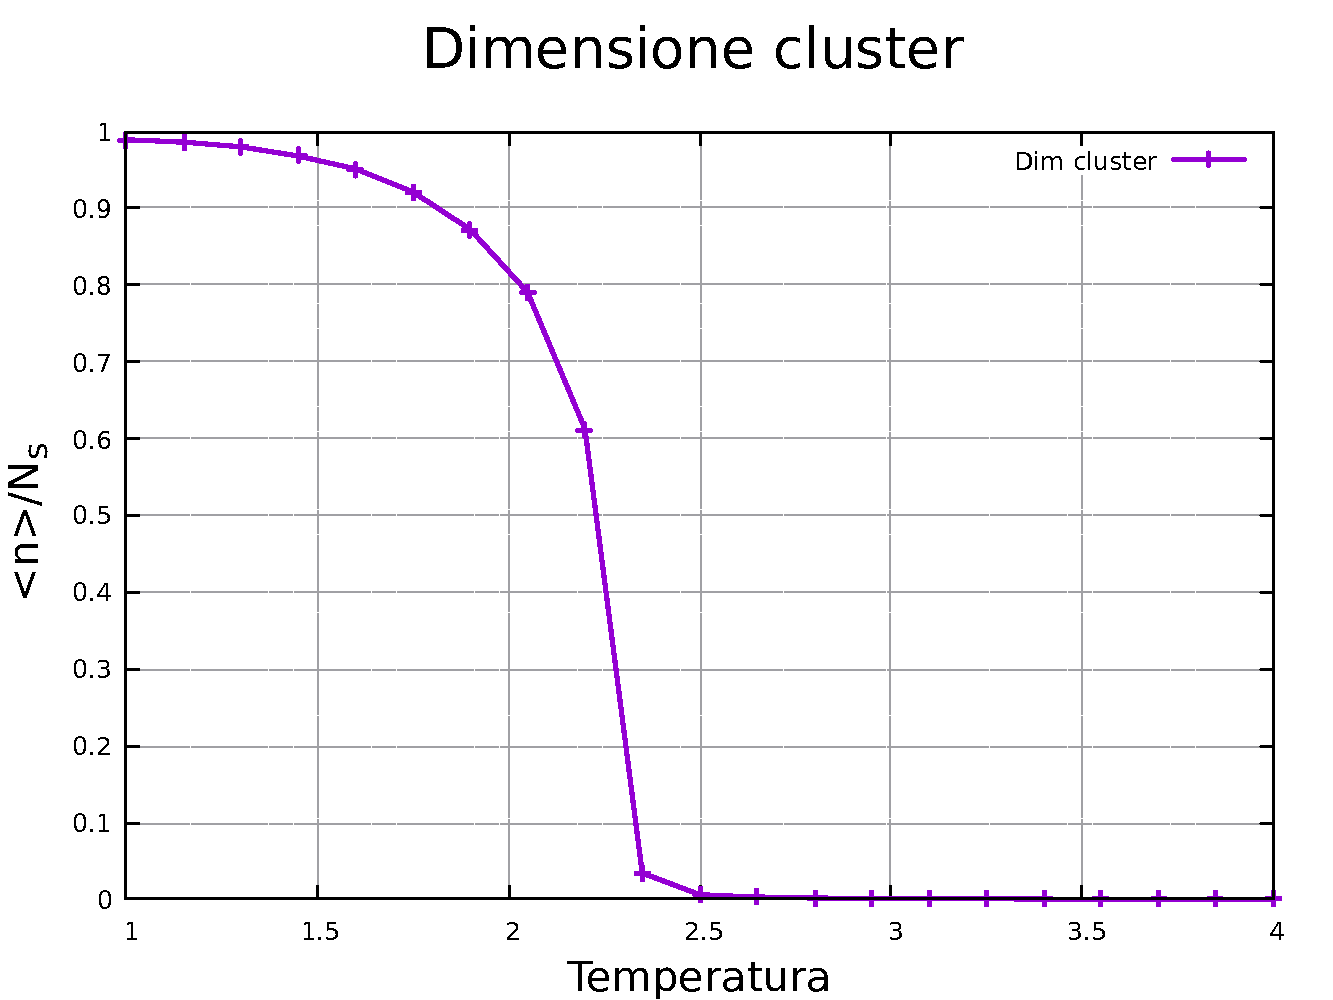
\includegraphics[width=0.75\textwidth]{Immagini/MC_meth/dim_clW.pdf}
    \caption{Frazione di reticolo ricoperta dal cluster in funzione della temperatura.}
    \label{fig: dim_clW}
\end{figure}

L'algoritmo nella sua interezza è costituito dai seguenti passi:

\begin{itemize}[label=$\diamond$] 
    \item si seleziona casualmente uno spin facente parte del reticolo
    \item si prendono in considerazione i primi vicini di quello spin. Se essi sono rivolti nella stessa direzione dello spin 
    selezionato in partenza, aggiungerli al cluster con probabilità data da \eqref{eq: padd_cluster}
    \item per ogni spin che è stato aggiunto allo step precedente, si considerano i primi vicini e si procede con la stessa metodologia. 
    Si continua fino a quando tutti i primi vicini degli spin facenti parte il cluster sono stati presi in considerazione per una possibile 
    inclusione.
    \item si invertono tutti gli spin che costituiscono il cluster. Questo processo avviene con probabilità uno, ossia viene sempre effettuato.
\end{itemize}

Questo algoritmo rispetta sia il bilancio dettagliato che l'ergodicità. La sua particolarità di lavorare su più spin alla volta consente di 
ridurre l'esponente $z$ di un fattore 10, dato che per il modello di Ising 2D è pari a $z\,=\,0.25 \pm 0.01$ \cite{MCM}.


\begin{minted}[frame=lines, fontsize=\small, bgcolor=blue!10, breaklines = true]{nim}
proc wolffMove*(modIsing: var seq[seq[int]], rg: var PCG, temp: float32, acc: float32, nspin: int): int = 
# Algoritmo di Wolff per evolvere il modello di Ising 2D

    var 
        appo: int
        conta: int
        test: IsingCoord
        clusterSize:int = 0
        stack: seq[IsingCoord] = @[]
        padd = 1 - exp(-2*acc/temp)

        # Variabili per coordinate spin
        randSpin, upNeigh, downNeigh, leftNeigh, rightNeigh: IsingCoord

    # Valuto casualmente spin
    randSpin = rg.newRandomCoord(nspin)
    stack.add(randSpin)

    # Salvo valore iniziale spin (per successivi confronti) e poi inverto spin
    appo = modIsing[randSpin.xcoor][randSpin.ycoor]
    modIsing[randSpin.xcoor][randSpin.ycoor] = -appo

    # Continuo fino a quando non ho controllato tutte le possibilità
    while stack.len() > 0:
        test = stack.pop
        clusterSize += 1

        # Valuto quali siano i primi vicini
        upNeigh = newCoord(test.xcoor, (test.ycoor + 1) mod nspin)
        downNeigh = newCoord(test.xcoor, (test.ycoor + nspin - 1) mod nspin)
        leftNeigh = newCoord((test.xcoor + 1) mod nspin, test.ycoor)
        rightNeigh = newCoord((test.xcoor + nspin - 1) mod nspin, test.ycoor)

        # Aggiungo al cluster solo se hanno lo stesso orientamento dello spin di partenza
        if modIsing[upNeigh.xcoor][upNeigh.ycoor] == appo and rg.rand() < padd:
            modIsing[upNeigh.xcoor][upNeigh.ycoor] = -appo
            stack.add(upNeigh);

        if modIsing[downNeigh.xcoor][downNeigh.ycoor] == appo and rg.rand() < padd:
            modIsing[downNeigh.xcoor][downNeigh.ycoor] = -appo
            stack.add(downNeigh);

        if modIsing[rightNeigh.xcoor][rightNeigh.ycoor] == appo and rg.rand() < padd:
            modIsing[rightNeigh.xcoor][rightNeigh.ycoor] = -appo
            stack.add(rightNeigh);

        if modIsing[leftNeigh.xcoor][leftNeigh.ycoor] == appo and rg.rand() < padd:
            modIsing[leftNeigh.xcoor][leftNeigh.ycoor] = -appo
            stack.add(leftNeigh);
            
    
    return clusterSize

\end{minted}    
    
\newpage
\section{Simulazioni modello di Ising 1D}

Sono state simulate catene di spin sia in assenza che in presenza di campo magnetico. Nelle seguenti sezioni è possibile consultare 
i risultati ottenuti in entrambe le casistiche.

\newpage

\newpage
\section{Simulazioni modello di Ising 2D}

%-----------------------------------------%
%				Prima slide				  %
%	   Caratterizzazione metropolis   	  %
%-----------------------------------------%
\begin{frame}
    \frametitle{Caratterizzazione con metropolis}
    \framesubtitle{}

    \begin{columns}
        \begin{column}{0.33\textwidth}
            \begin{block}{Termalizzazione}

                \begin{itemize}[itemsep=0.5em, label=$\diamond$]
                    \item $t_{ter}$ maggiori per $T \simeq T_c$
                    \item $t_{ter}^{max}\,\simeq\,500$ sweeps
                \end{itemize}

                \vspace{0.5cm}

                \centering
                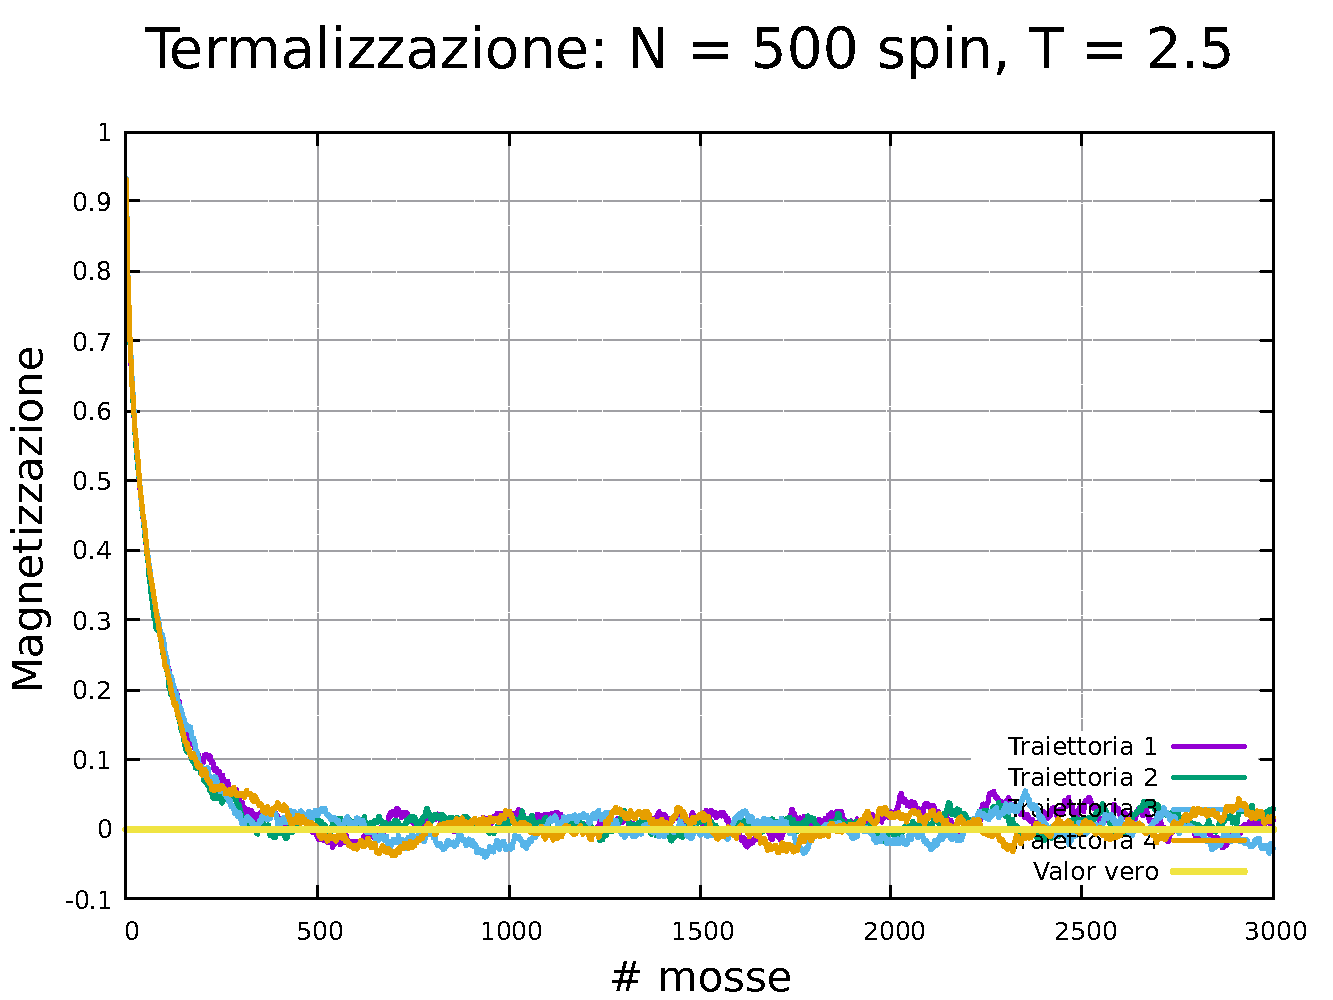
\includegraphics[width=\textwidth]{Immagini/simIsing2D/term_500_2.5.pdf}
            
            \end{block}
        \end{column}
    
        \begin{column}{0.33\textwidth}
            \begin{block}{Auto-correlazione}

                \begin{itemize}[itemsep=0.5em, label=$\diamond$]
                    \item $t_{c}$ maggiori per $T \simeq T_c$
                    \item $t_{c}^{max}\,\simeq\,400$ sweeps
                \end{itemize}

                \vspace{0.5cm}

                \centering
                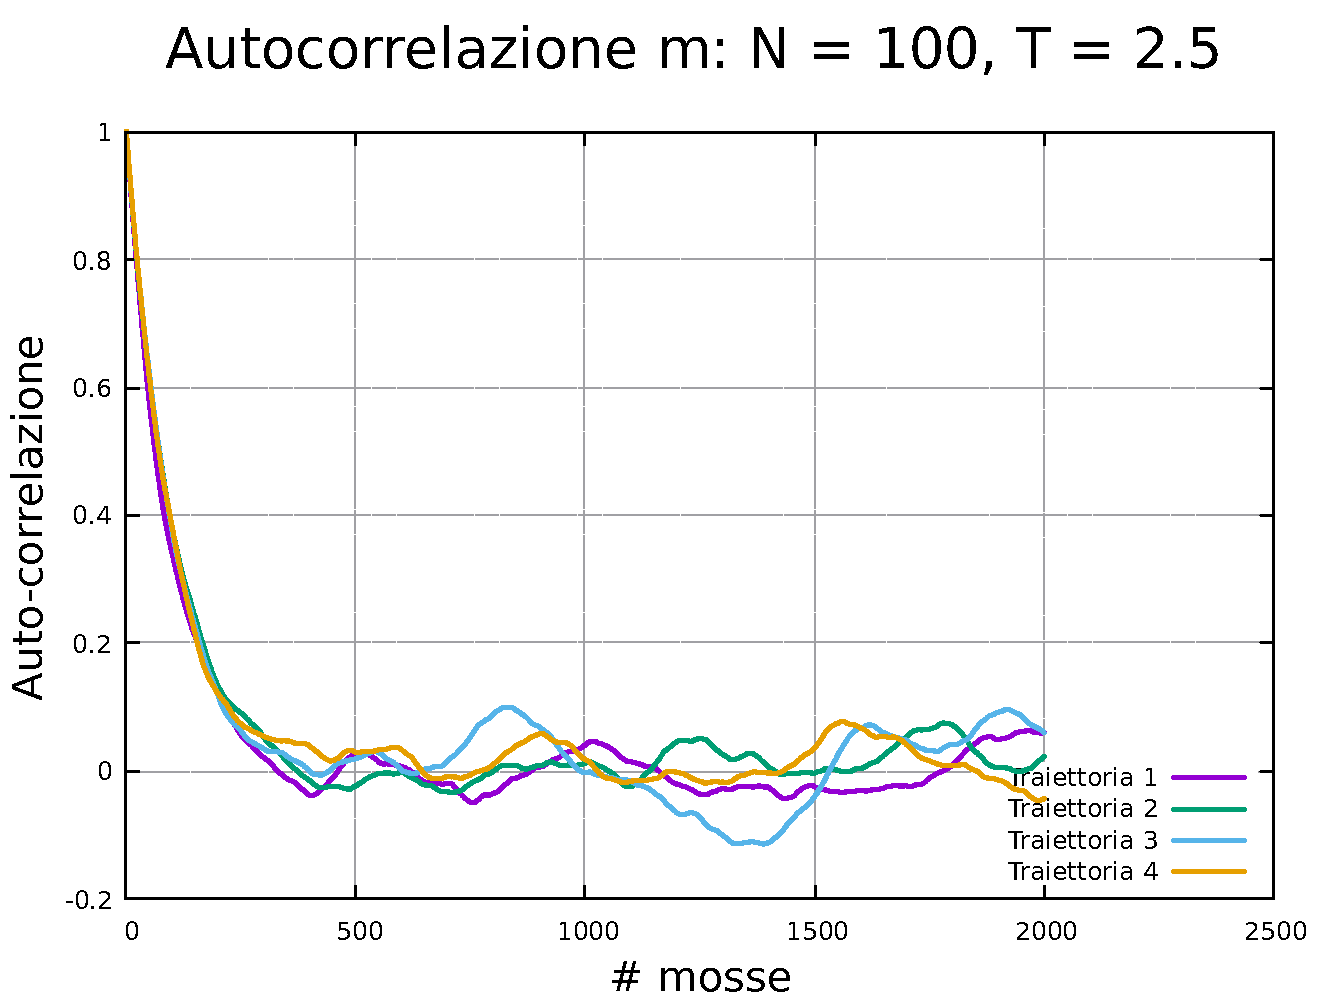
\includegraphics[width=\textwidth]{Immagini/simIsing2D/auto_100_2.5.pdf}
            
            \end{block}
        \end{column}

        \begin{column}{0.33\textwidth}
            \begin{block}{Blocchi}
                \begin{itemize}[itemsep=0.5em, label=$\diamond$]
                    \item $l_{blk}$ maggiori per $T \simeq T_c$
                    \item $l_{blk}^{max}\,\simeq\,1000$ sweeps
                \end{itemize}

                \vspace{0.5cm}

                \centering
                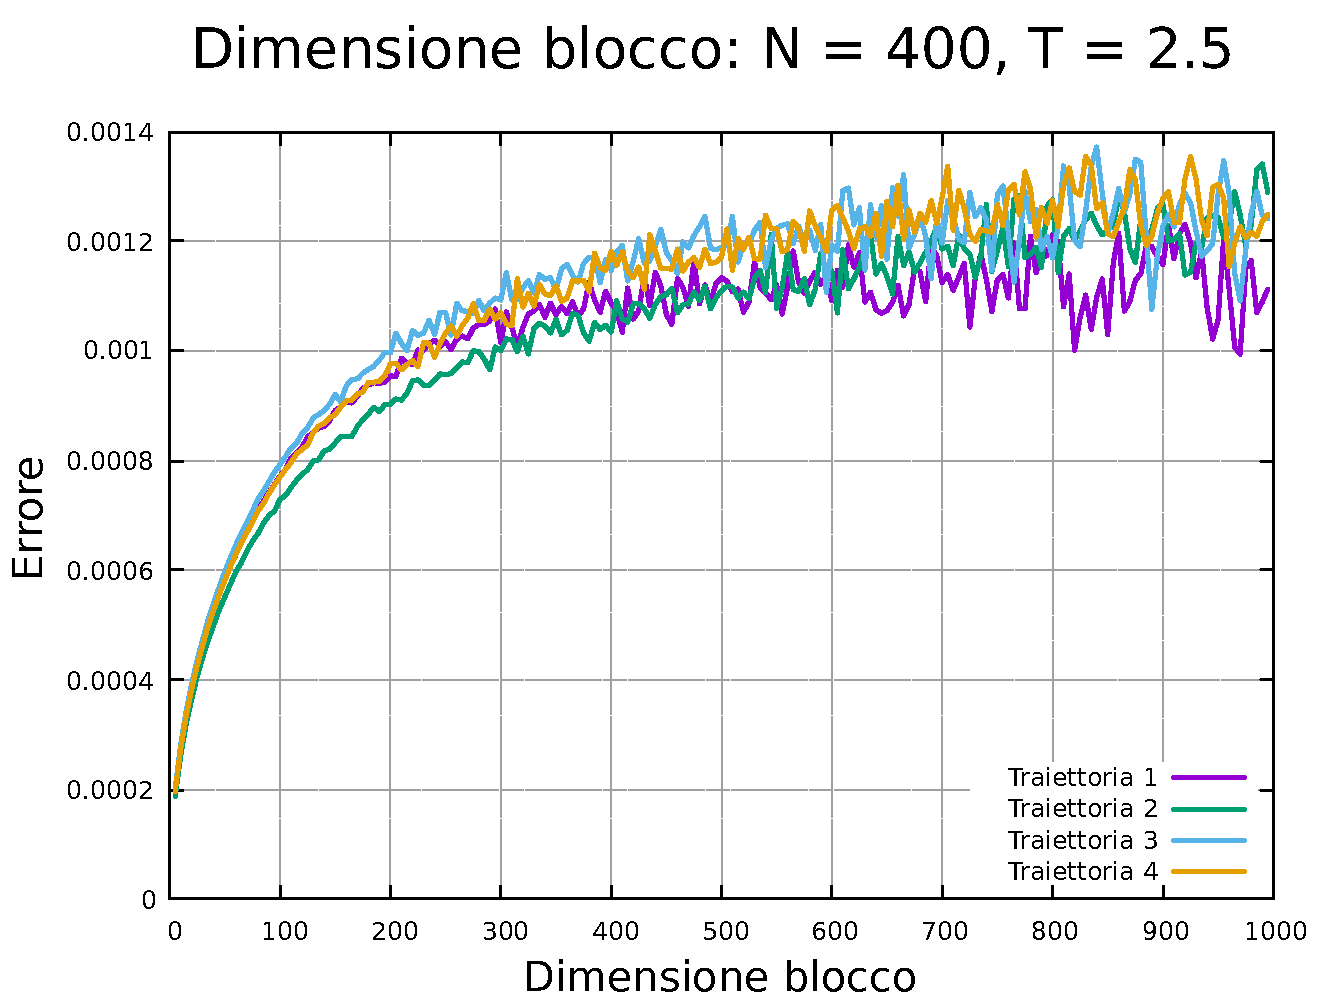
\includegraphics[width=\textwidth]{Immagini/simIsing2D/err_400_2.5.pdf}
            \end{block}        
        \end{column}
    \end{columns}
\end{frame}



%-----------------------------------------%
%		        Seconda slide	    	  %
%	      Caratterizzazione wolff   	  %
%-----------------------------------------%
\begin{frame}
    \frametitle{Caratterizzazione con Wolff}
    \framesubtitle{}

    \begin{columns}
        \begin{column}{0.33\textwidth}
            \begin{block}{Termalizzazione}
            
            \end{block}
        \end{column}
    
        \begin{column}{0.33\textwidth}
            \begin{block}{Auto-correlazione}

            \end{block}
        \end{column}

        \begin{column}{0.33\textwidth}
            \begin{block}{Blocchi}

            \end{block}        
        \end{column}
    \end{columns}
\end{frame}



%-----------------------------------------%
%			  Terza slide				  %
%	   Studio della magnetizzazione   	  %
%-----------------------------------------%
\begin{frame}
    \frametitle{Magnetizzazione}
    \framesubtitle{}

    \begin{columns}
        \begin{column}{0.6\textwidth}

            \centering
            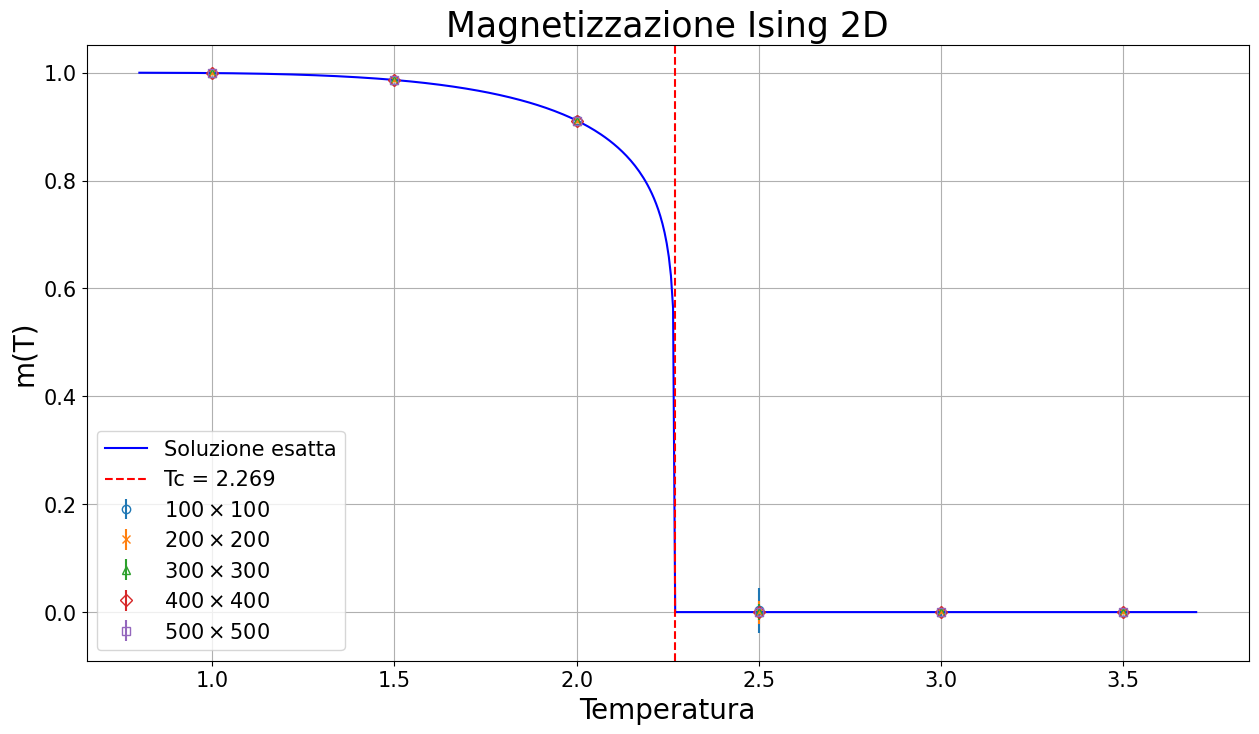
\includegraphics[width=\textwidth]{Immagini/simIsing2D/magn.png}

        \end{column}
    
        \begin{column}{0.4\textwidth}

                \begin{itemize}[itemsep=0.5em, label=$\diamond$]
                    \item Magnetizzazione spontanea per $T\,<\,T_c$
                    \item Transizione di fase a $T_c$
                \end{itemize}
            
        \end{column}
    \end{columns}

    \centering
    \begin{tikzpicture}[thick, scale=1.2]
        \draw[->, line width=1mm] (0, 0) -- (10, 0);
        
        \node[below] at (0, 0) {Ferromagnetico};
        \node[below] at (10, 0) {Paramagnetico};
        
        \draw[fill=black] (5, 0) circle (2pt); 
        \node[above] at (5, 0) {$T_c$}; 
    \end{tikzpicture}

\end{frame}



%-----------------------------------------%
%			  Quarta slide				  %
%	   Studio dell'energia interna   	  %
%-----------------------------------------%
\begin{frame}
    \frametitle{Energia}
    \framesubtitle{}

    \begin{columns}
        \begin{column}{0.6\textwidth}

            \centering
            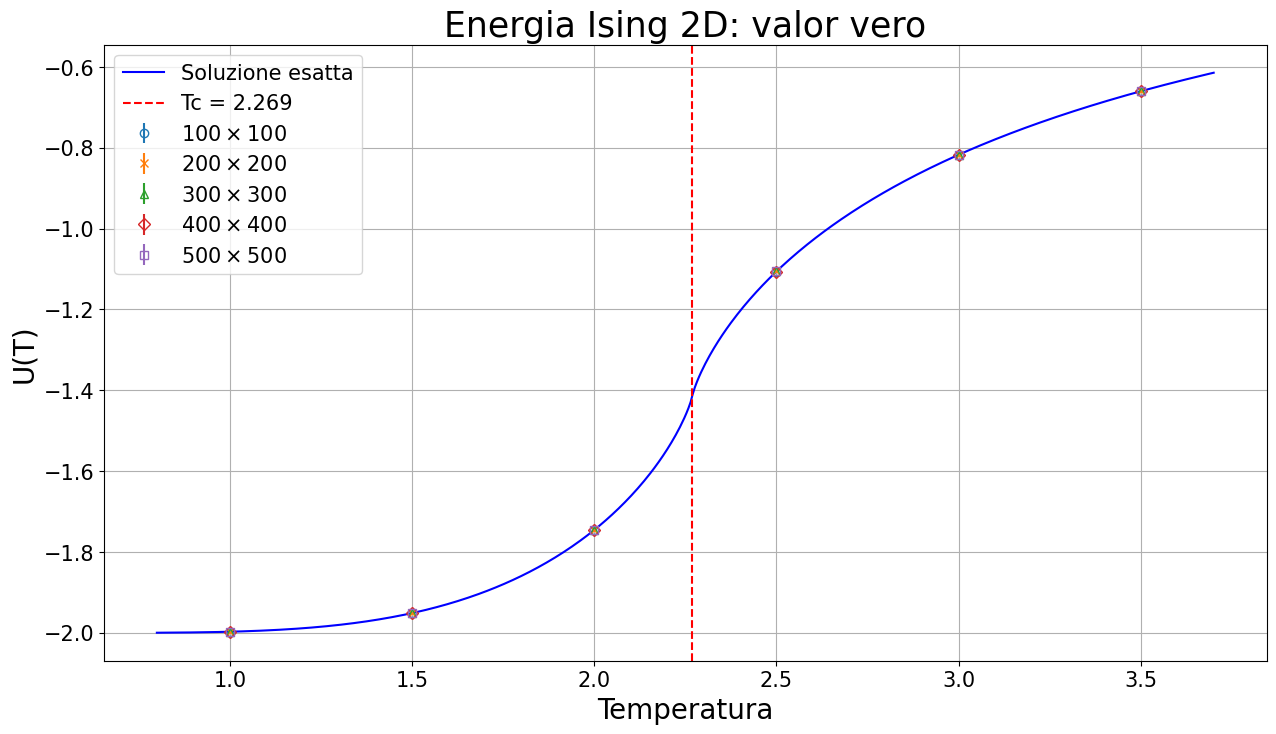
\includegraphics[width=\textwidth]{Immagini/simIsing2D/ene.png}

        \end{column}
    
        \begin{column}{0.4\textwidth}


                \begin{itemize}[itemsep=0.5em, label=$\diamond$]
                    \item copro tutto il reticolo con due legami per spin
                    \item picco del calore specifico a $T_c$
                \end{itemize}
            
        \end{column}
    \end{columns}

    \vspace{0.5cm}
    \centering
    $U\,=\,-NJ\coth{\left(2\beta J\right)}\left\{1\,+\,\frac{2}{\pi}\left[2\tanh^2\left(2\beta J\right)\,-\,1\right]\int_0^{\pi/2}\frac{d\phi}{\sqrt{1\,-\,k^2\sin^2{\left(\phi\right)}}}\right\}$

\end{frame}



%-----------------------------------------%
%		  	  Quinta slide - A			  %
%	      Studio della T critica    	  %
%-----------------------------------------%
\begin{frame}
    \frametitle{Dipendenza da $J$}
    \framesubtitle{}

    \begin{columns}
        \begin{column}{0.6\textwidth}

            \centering
            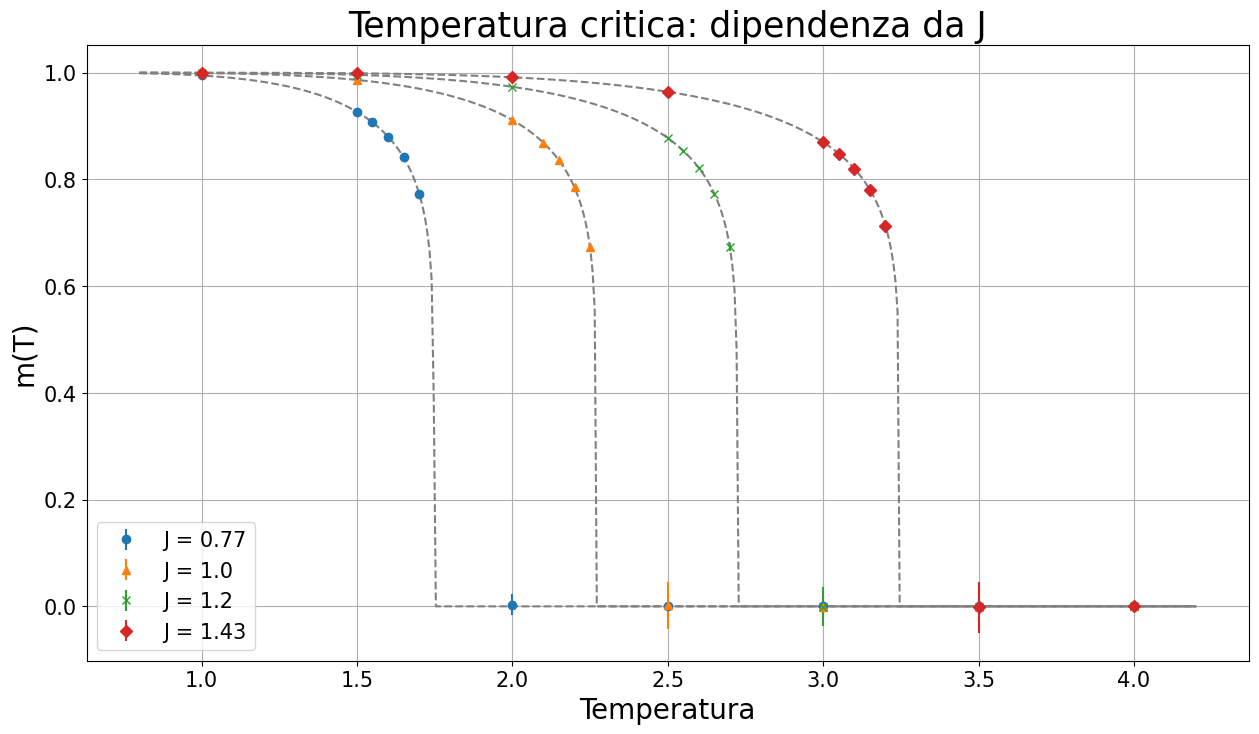
\includegraphics[width=\textwidth]{Immagini/simIsing2D/dipJ_Tc.png}

        \end{column}
    
        \begin{column}{0.4\textwidth}

                \begin{itemize}[itemsep=0.5em, label=$\diamond$]
                    \item Aumenta $J$, aumenta $T_c$
                    \item Presenza o meno di ordine dipende dall'intensità dell'interazione
                \end{itemize}
            
        \end{column}
    \end{columns}

\end{frame}



%-----------------------------------------%
%			Quinta slide - B			  %
%	   Studio del calore specifico   	  %
%-----------------------------------------%
\begin{frame}
    \frametitle{Regione critica}
    \framesubtitle{}

    \begin{columns}
        \begin{column}{0.5\textwidth}

            \centering
            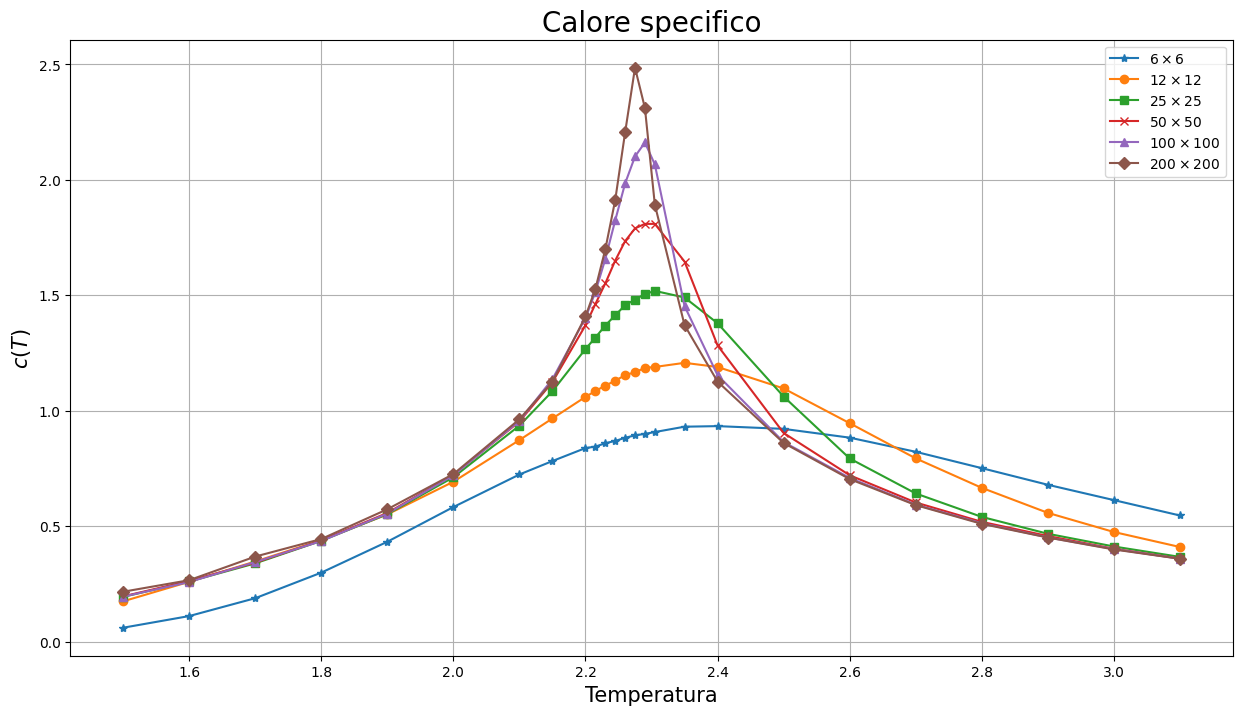
\includegraphics[width=\textwidth]{Immagini/simIsing2D/cp_zCrit.png}

        \end{column}
    
        \begin{column}{0.5\textwidth}
            
        \end{column}
    \end{columns}

\end{frame}



%-----------------------------------------%
%		   	  Settima slide				  %
%	     Studio con coarse graining   	  %
%-----------------------------------------%
\begin{frame}
    \frametitle{Coarse graining}
    \framesubtitle{}

    \centering
    \begin{tikzpicture}
        \node (img1) at (-1,0) {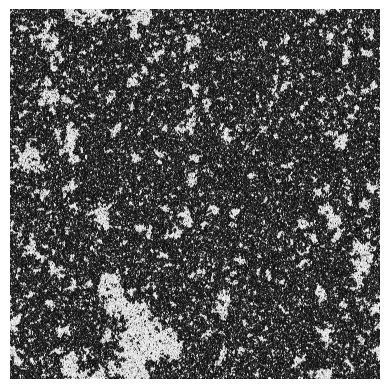
\includegraphics[width=0.4\textwidth]{Immagini/simIsing2D/cg_10000_Tc.png}};
        
        \node (img2) at (7,0) {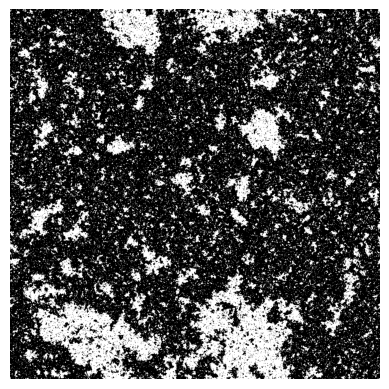
\includegraphics[width=0.4\textwidth]{Immagini/simIsing2D/cg_1000_Tc.png}};
        
        \draw[->,thick] (img1.east)  -- node[above] {CG} (img2.west);
    \end{tikzpicture}
    
\end{frame}



%-----------------------------------------%
%		   	   Ottava slide				  %
%	      Dimensione dei clusters   	  %
%-----------------------------------------%
\begin{frame}
    \frametitle{Dimensioni cluster}
    \framesubtitle{}

    \begin{columns}
        \begin{column}{0.6\textwidth}

            \centering
            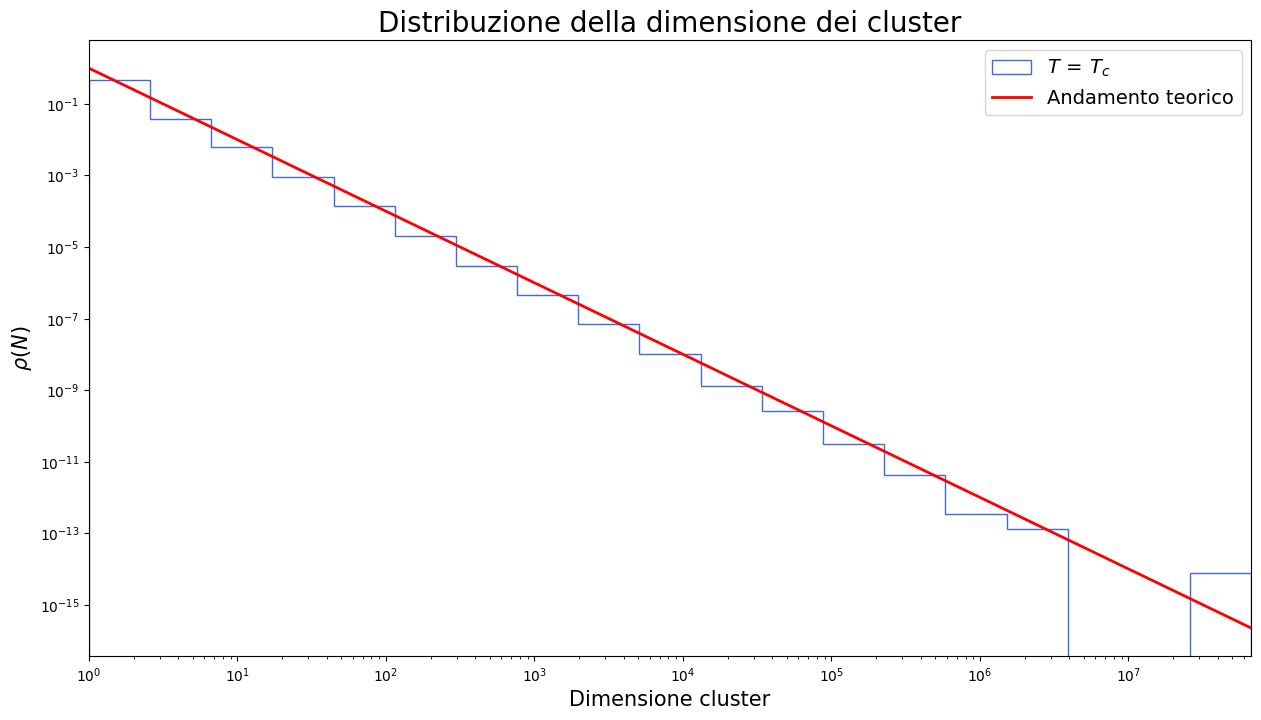
\includegraphics[width=\textwidth]{Immagini/simIsing2D/dimCl_Tc.png}

        \end{column}
    
        \begin{column}{0.4\textwidth}


                \begin{itemize}[itemsep=0.5em, label=$\diamond$]
                    \item $P\left(s\right) \propto s^{-\alpha}$
                    \item $\alpha \simeq 2$
                    \item perdita di un parametro di scala
                \end{itemize}
            
        \end{column}
    \end{columns}

    \centering
    \begin{tikzpicture}[thick, scale=1.2]
        \draw[->, line width=1mm] (0, 0) -- (10, 0);
        
        \node[below] at (0, 0) {grandi cluster};
        \node[below] at (10, 0) {piccoli cluster};
        
        \draw[fill=black] (5, 0) circle (2pt); 
        \node[above] at (5, 0) {$T_c$}; 
    \end{tikzpicture}
    
\end{frame}

\newpage
\appendix 


%-------------------------------------------%
%          Modello di Ising 1D              %
%-------------------------------------------%
\section{Modello di Ising 1D: $h\,=\,0.0$}
\subsection{Termalizzazione}

\vspace*{\fill}

\begin{figure}[htbp]
    \centering
    \begin{minipage}{0.45\textwidth}  
      \centering
      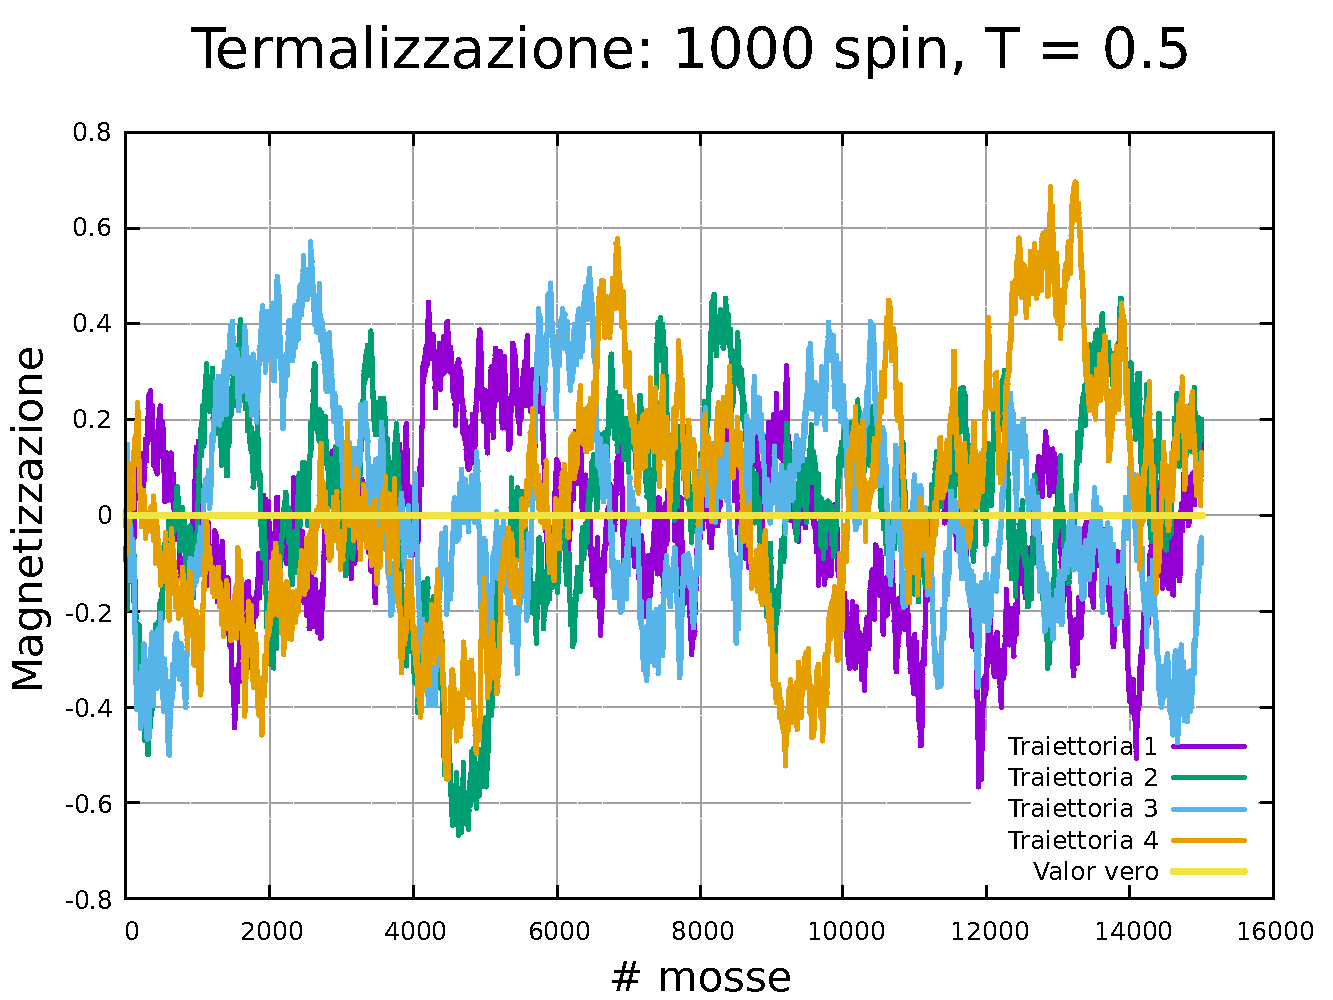
\includegraphics[page=1, width=\textwidth]{Immagini/simIsing1D/magn0.0/term/term_1000_0.5.pdf}
      \caption{$T\,=\,0.5$}
    \end{minipage}\hfill
    \begin{minipage}{0.45\textwidth}  
      \centering
      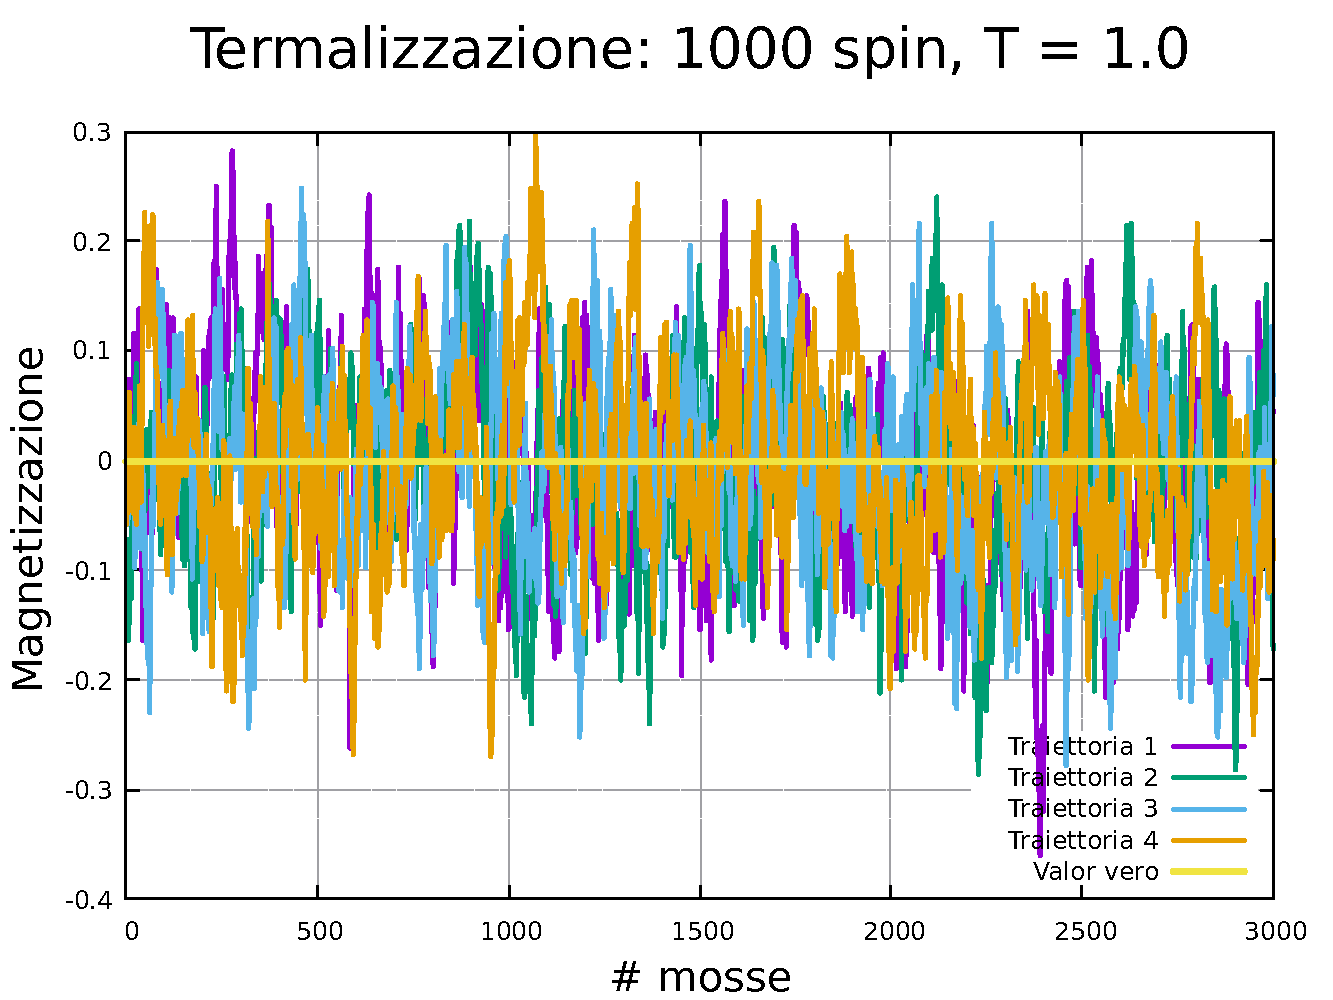
\includegraphics[page=1, width=\textwidth]{Immagini/simIsing1D/magn0.0/term/term_1000_1.0.pdf}
      \caption{$T\,=\,1.0$}
    \end{minipage}
    \vskip\baselineskip 
  
    \begin{minipage}{0.45\textwidth}  
      \centering
      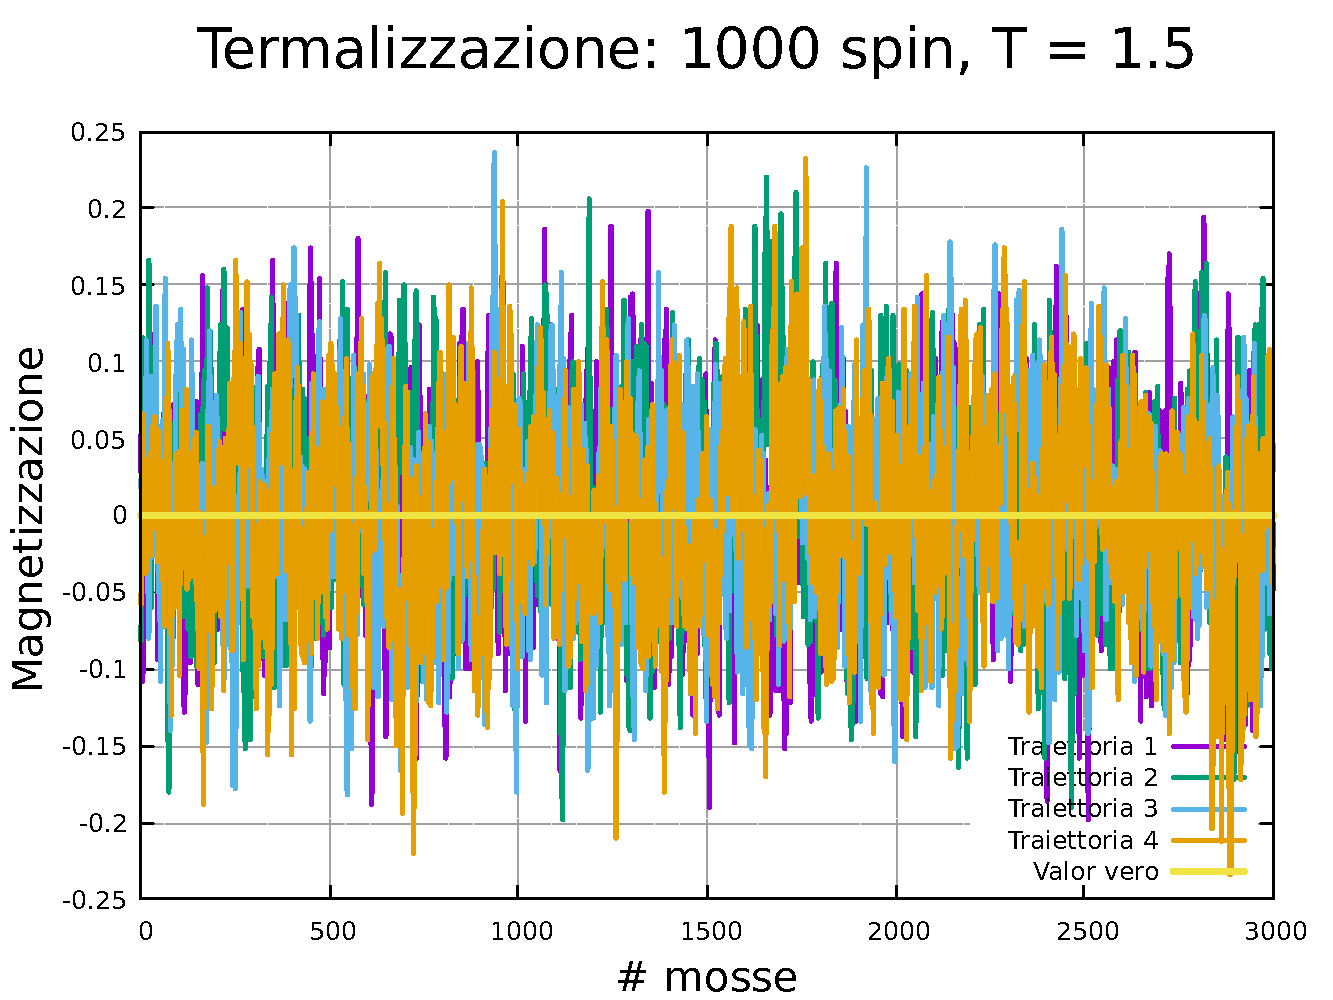
\includegraphics[page=1, width=\textwidth]{Immagini/simIsing1D/magn0.0/term/term_1000_1.5.pdf}
      \caption{$T\,=\,1.5$}
    \end{minipage}\hfill
    \begin{minipage}{0.45\textwidth}  
      \centering
      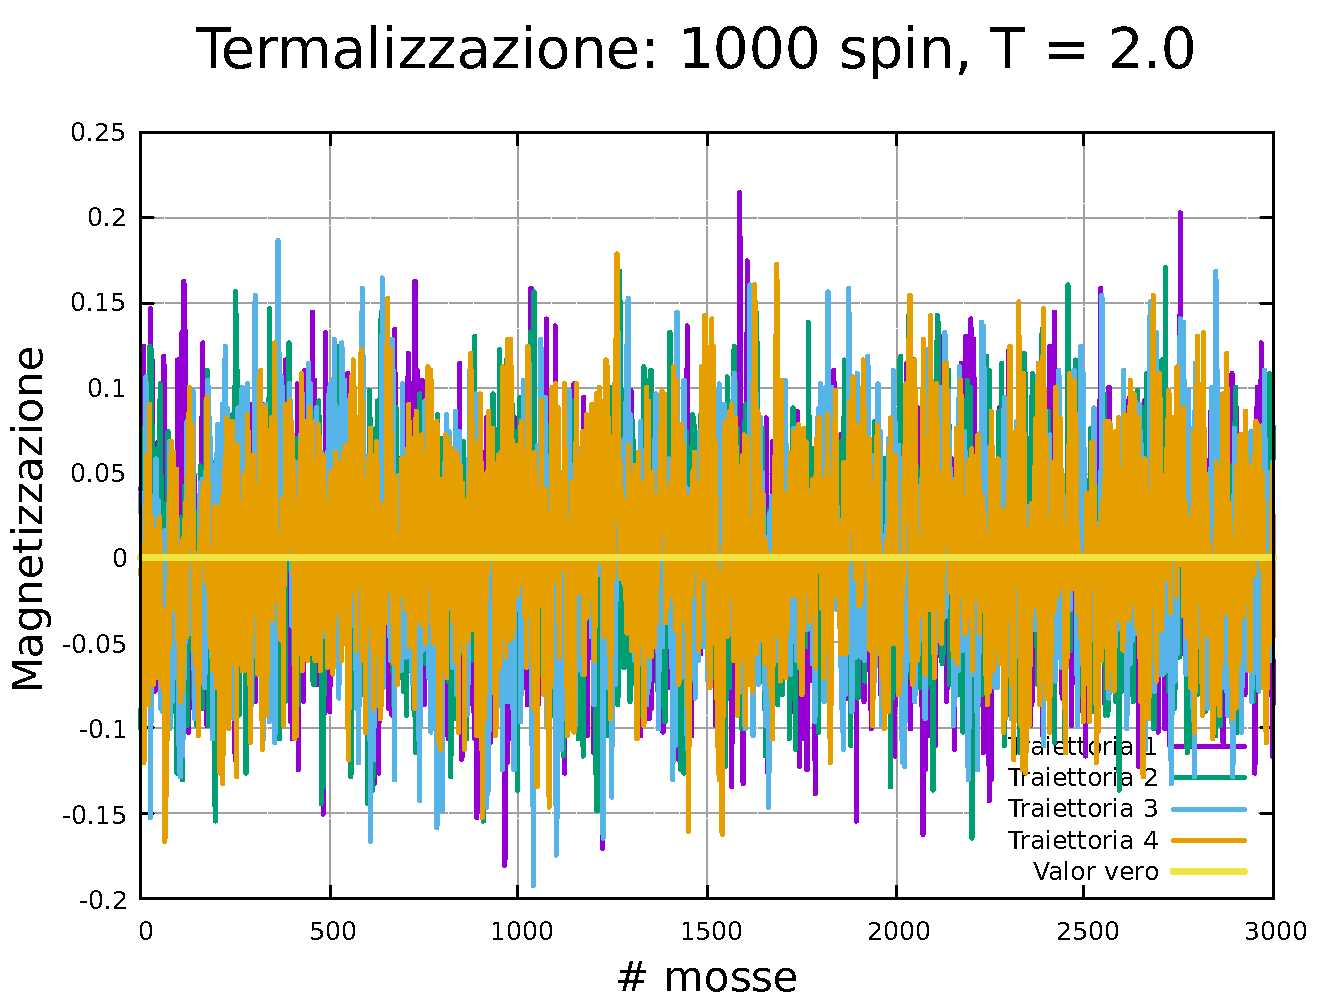
\includegraphics[page=1, width=\textwidth]{Immagini/simIsing1D/magn0.0/term/term_1000_2.0.pdf}
      \caption{$T\,=\,2.0$}
    \end{minipage}
    \caption{Studio della termalizzazione di un modello di Ising 1D costituito da 1000 spin.}
\end{figure}

\vspace*{\fill}

\newpage

\vspace*{\fill}

\begin{figure}[htbp]
    \centering
    \begin{minipage}{0.45\textwidth}  
      \centering
      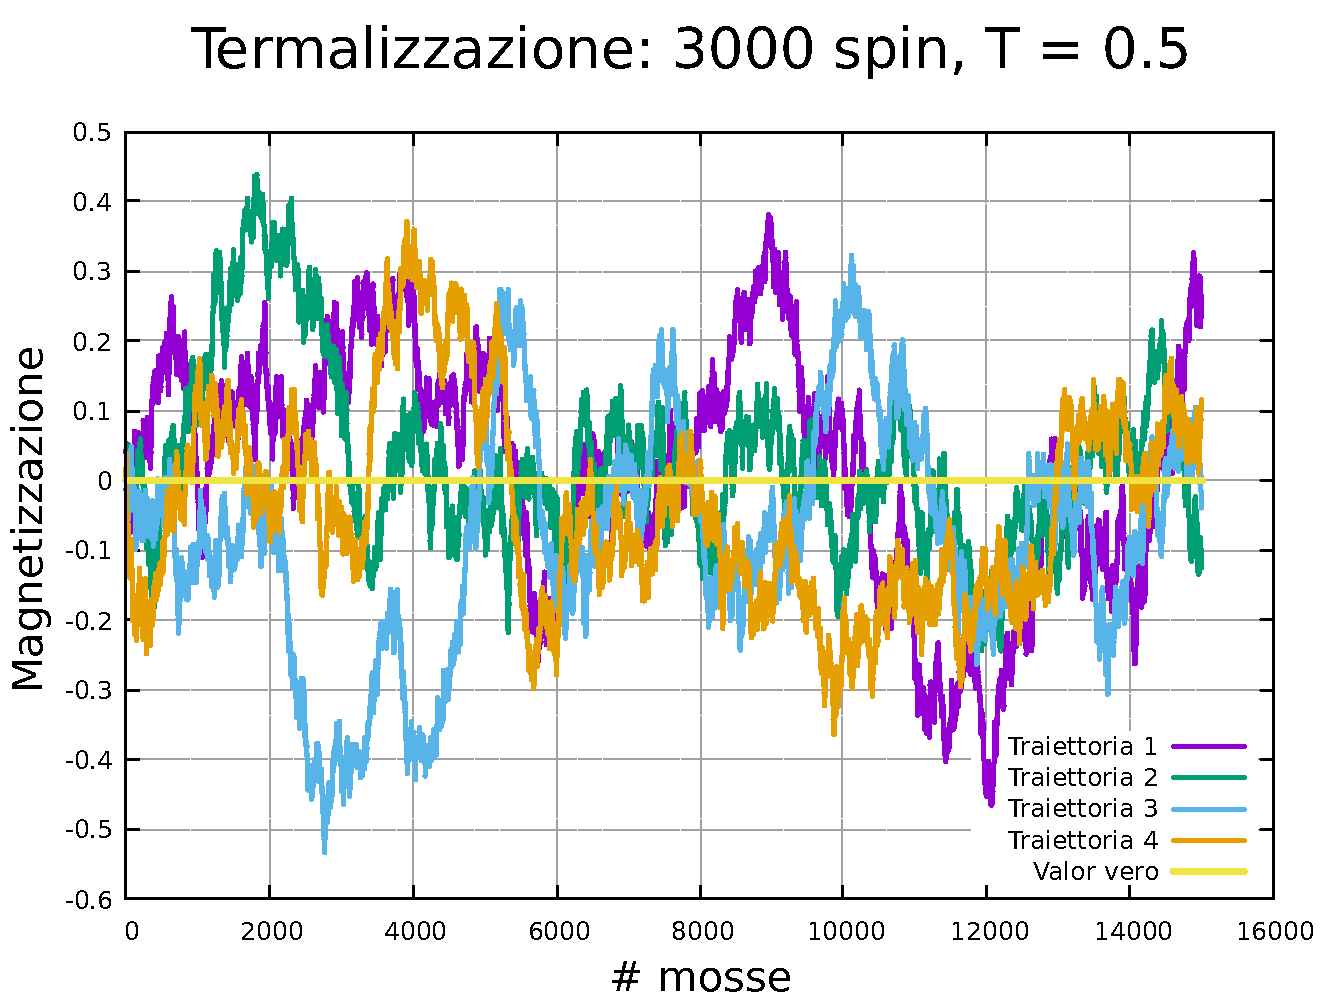
\includegraphics[page=1, width=\textwidth]{Immagini/simIsing1D/magn0.0/term/term_3000_0.5.pdf}
      \caption{$T\,=\,0.5$}
    \end{minipage}\hfill
    \begin{minipage}{0.45\textwidth}  
      \centering
      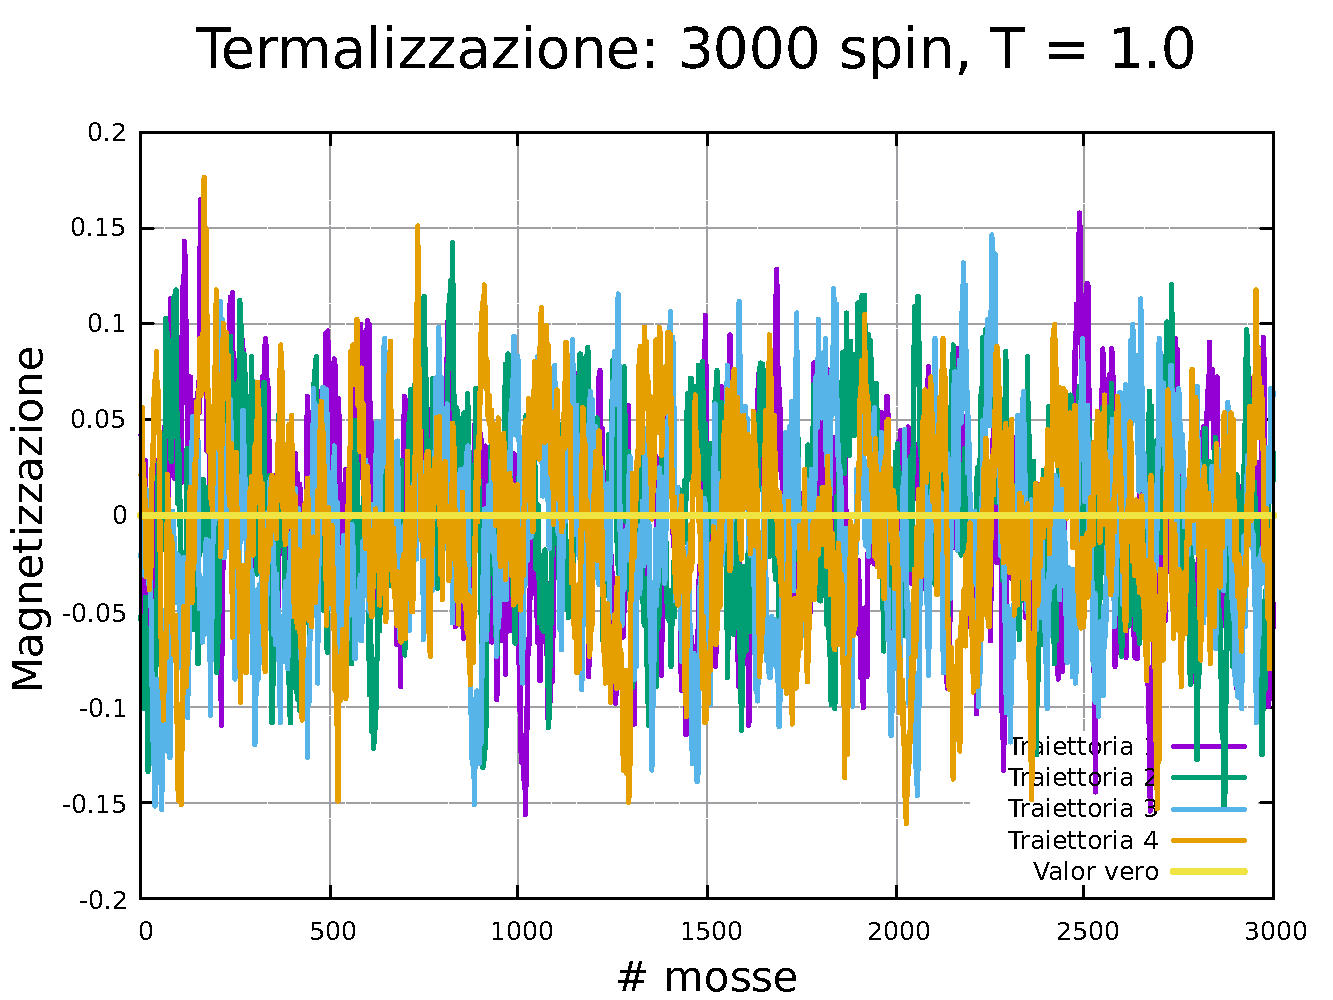
\includegraphics[page=1, width=\textwidth]{Immagini/simIsing1D/magn0.0/term/term_3000_1.0.pdf}
      \caption{$T\,=\,1.0$}
    \end{minipage}
    \vskip\baselineskip 
  
    \begin{minipage}{0.45\textwidth}  
      \centering
      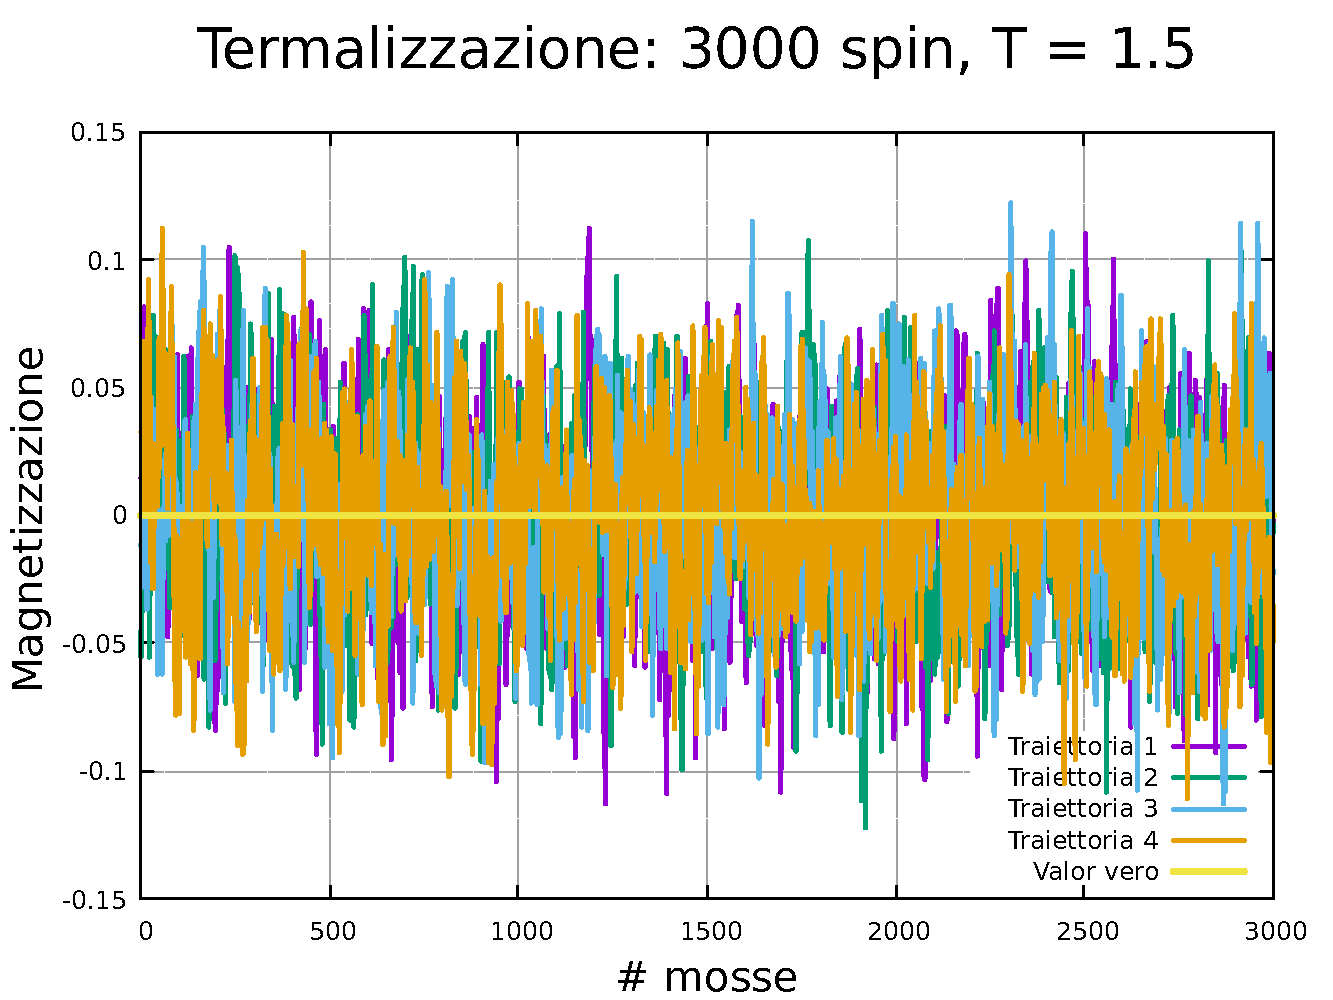
\includegraphics[page=1, width=\textwidth]{Immagini/simIsing1D/magn0.0/term/term_3000_1.5.pdf}
      \caption{$T\,=\,1.5$}
    \end{minipage}\hfill
    \begin{minipage}{0.45\textwidth}  
      \centering
      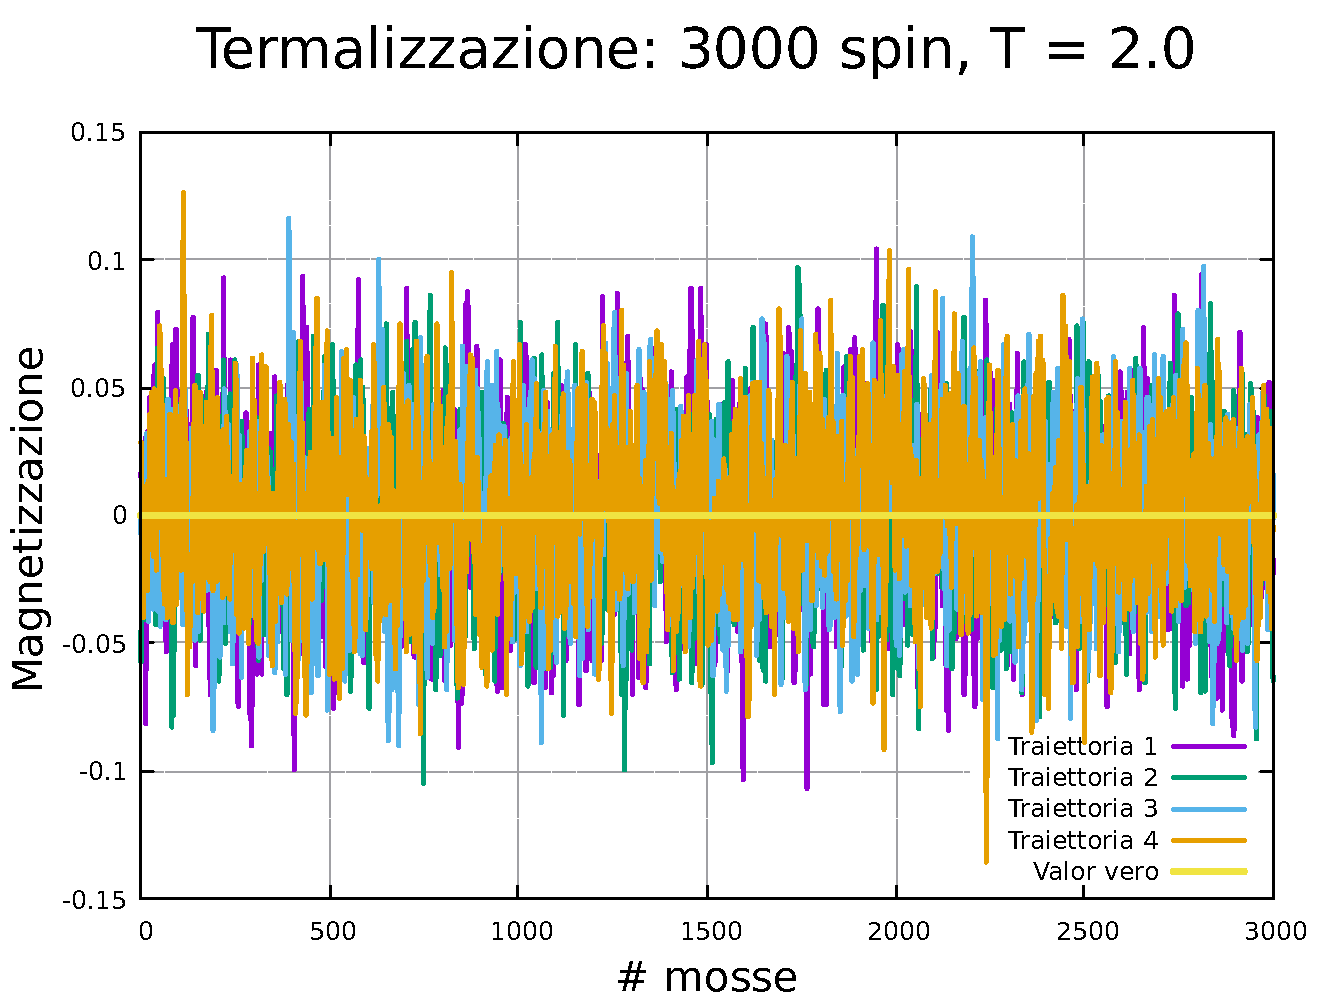
\includegraphics[page=1, width=\textwidth]{Immagini/simIsing1D/magn0.0/term/term_3000_2.0.pdf}
      \caption{$T\,=\,2.0$}
    \end{minipage}
    \caption{Studio della termalizzazione di un modello di Ising 1D costituito da 3000 spin.}
\end{figure}

\vspace*{\fill}

\newpage

\vspace*{\fill}

\begin{figure}[htbp]
    \centering
    \begin{minipage}{0.45\textwidth}  
      \centering
      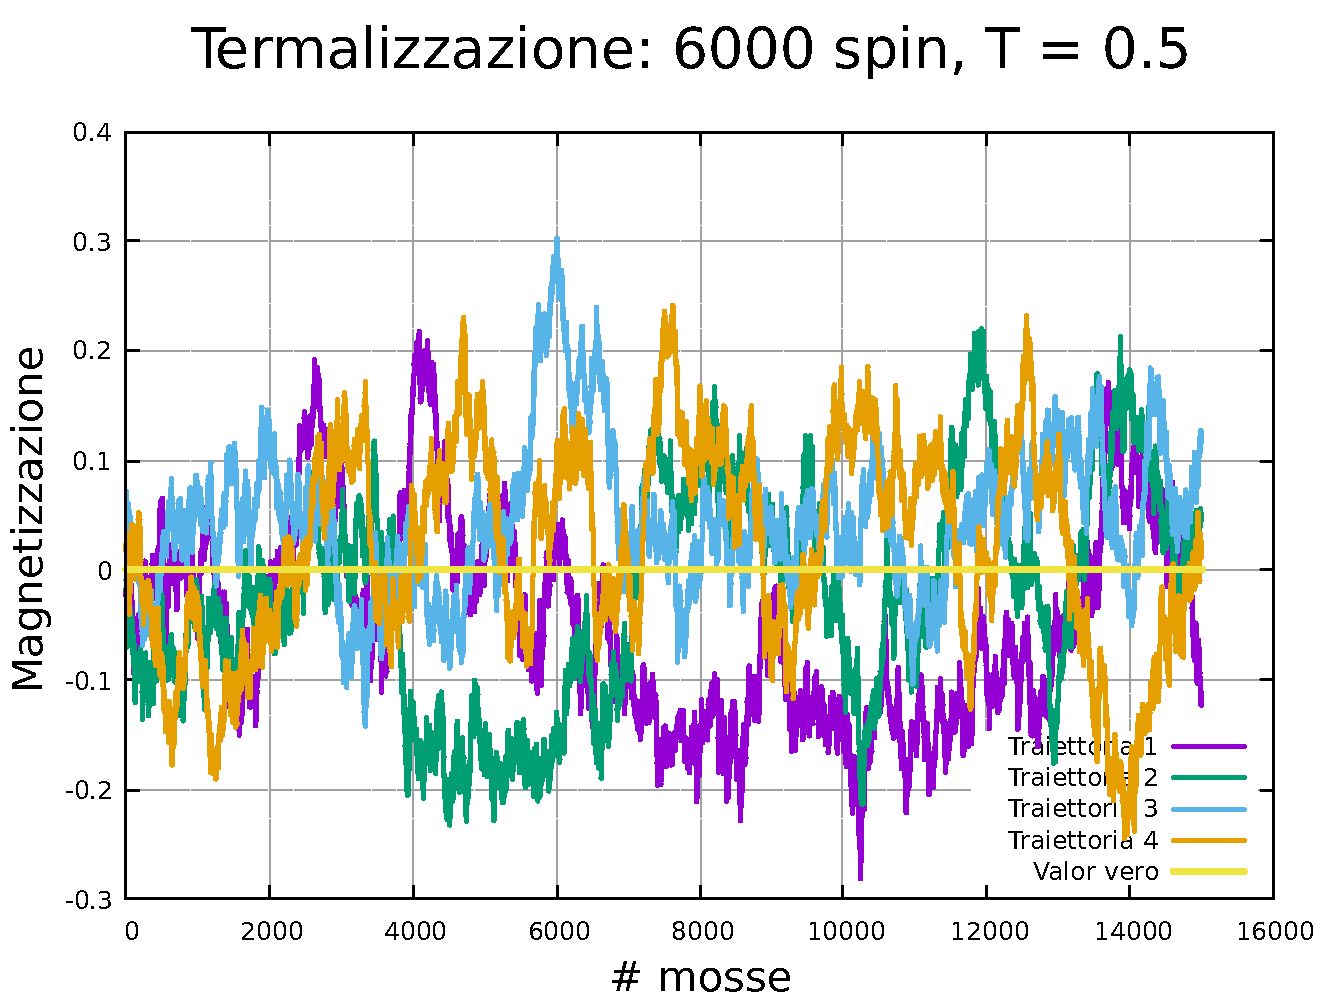
\includegraphics[page=1, width=\textwidth]{Immagini/simIsing1D/magn0.0/term/term_6000_0.5.pdf}
      \caption{$T\,=\,0.5$}
    \end{minipage}\hfill
    \begin{minipage}{0.45\textwidth}  
      \centering
      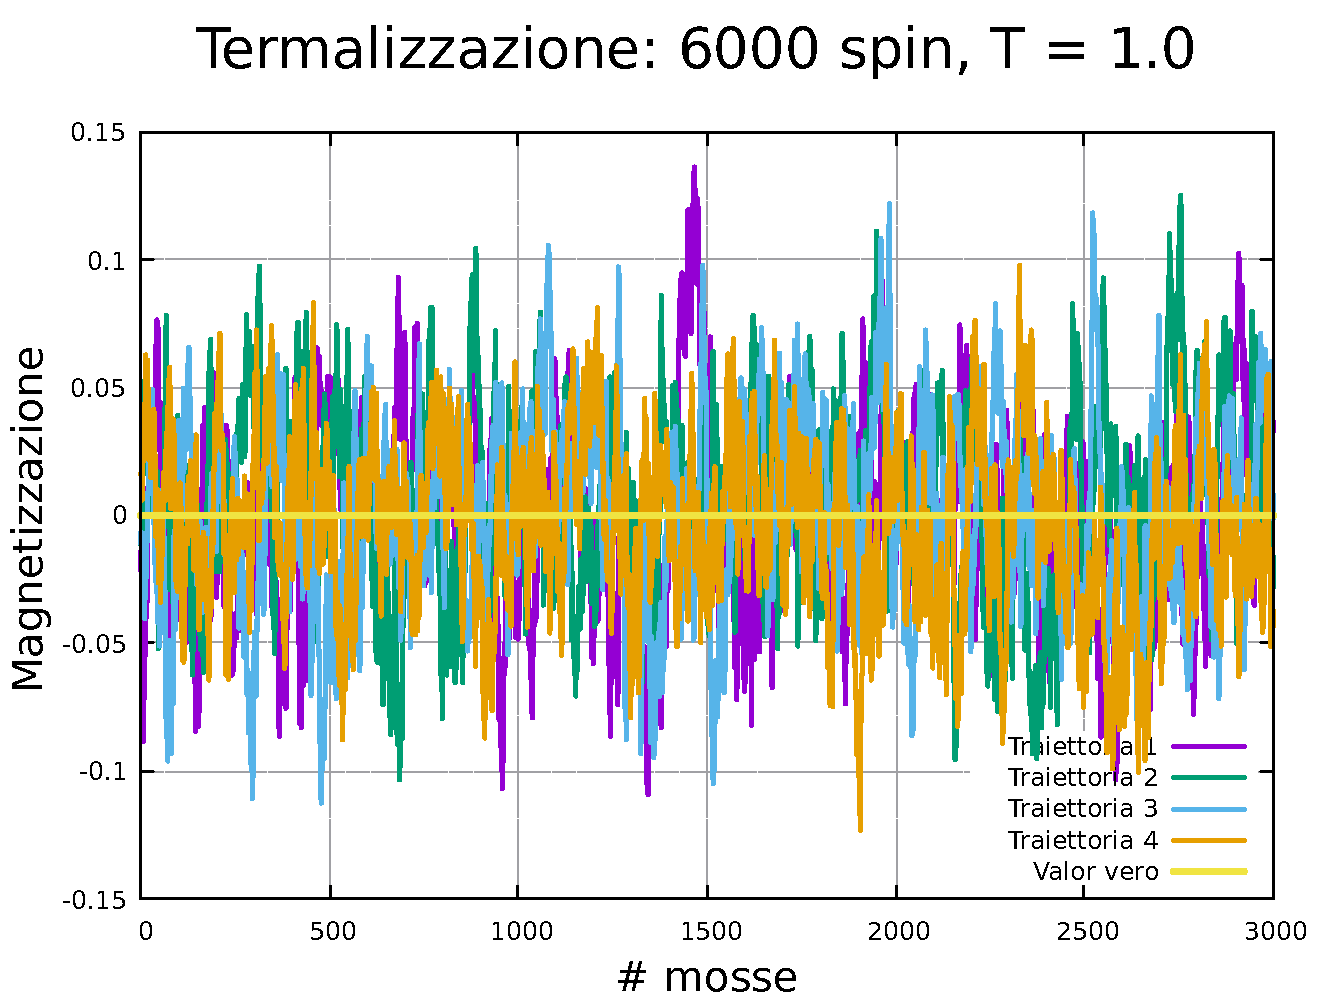
\includegraphics[page=1, width=\textwidth]{Immagini/simIsing1D/magn0.0/term/term_6000_1.0.pdf}
      \caption{$T\,=\,1.0$}
    \end{minipage}
    \vskip\baselineskip 
  
    \begin{minipage}{0.45\textwidth}  
      \centering
      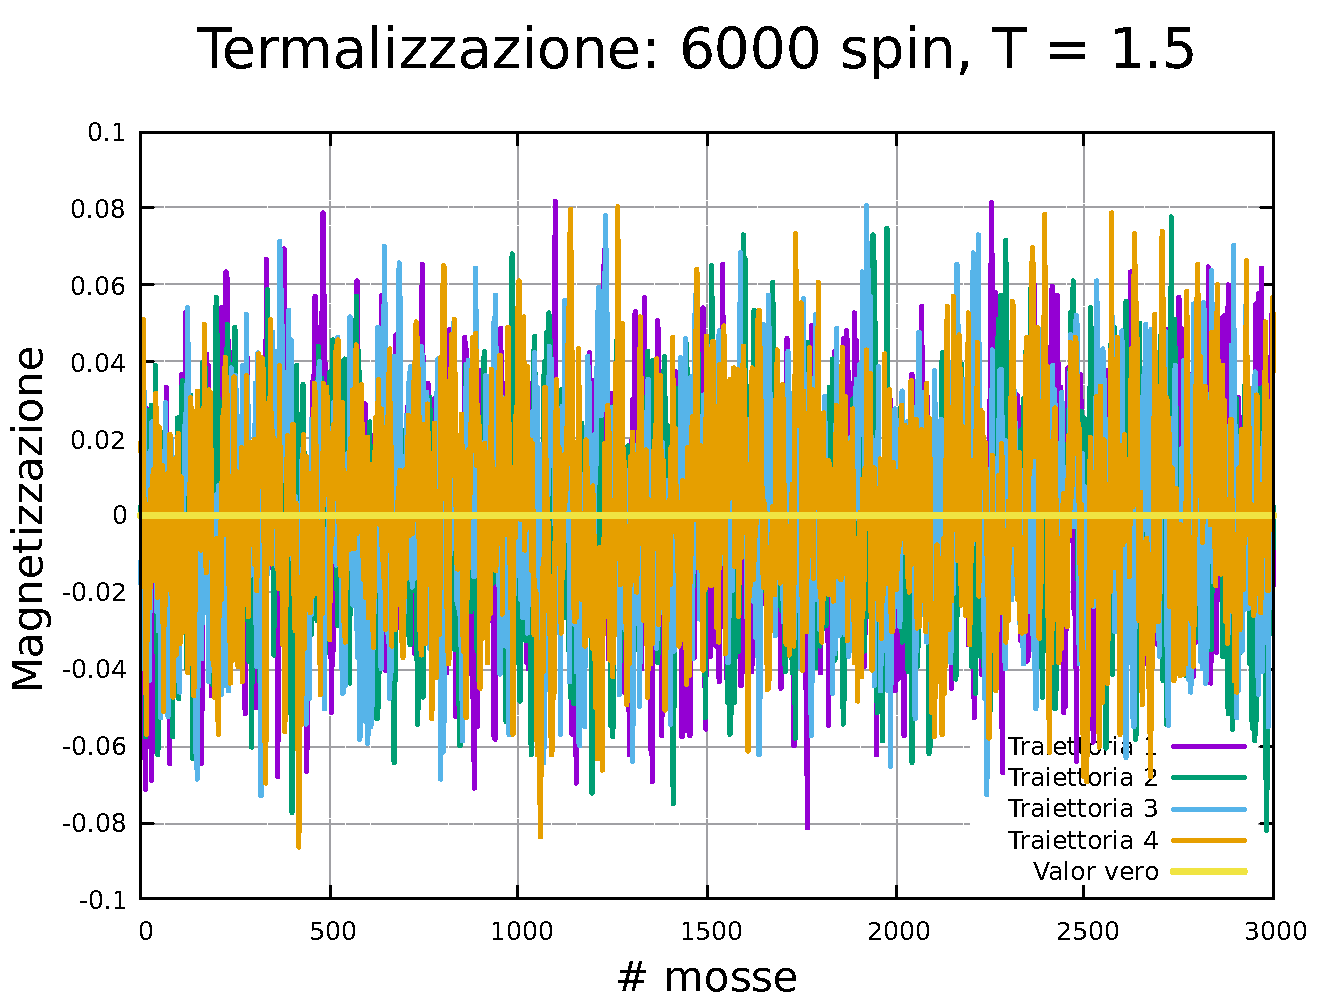
\includegraphics[page=1, width=\textwidth]{Immagini/simIsing1D/magn0.0/term/term_6000_1.5.pdf}
      \caption{$T\,=\,1.5$}
    \end{minipage}\hfill
    \begin{minipage}{0.45\textwidth}  
      \centering
      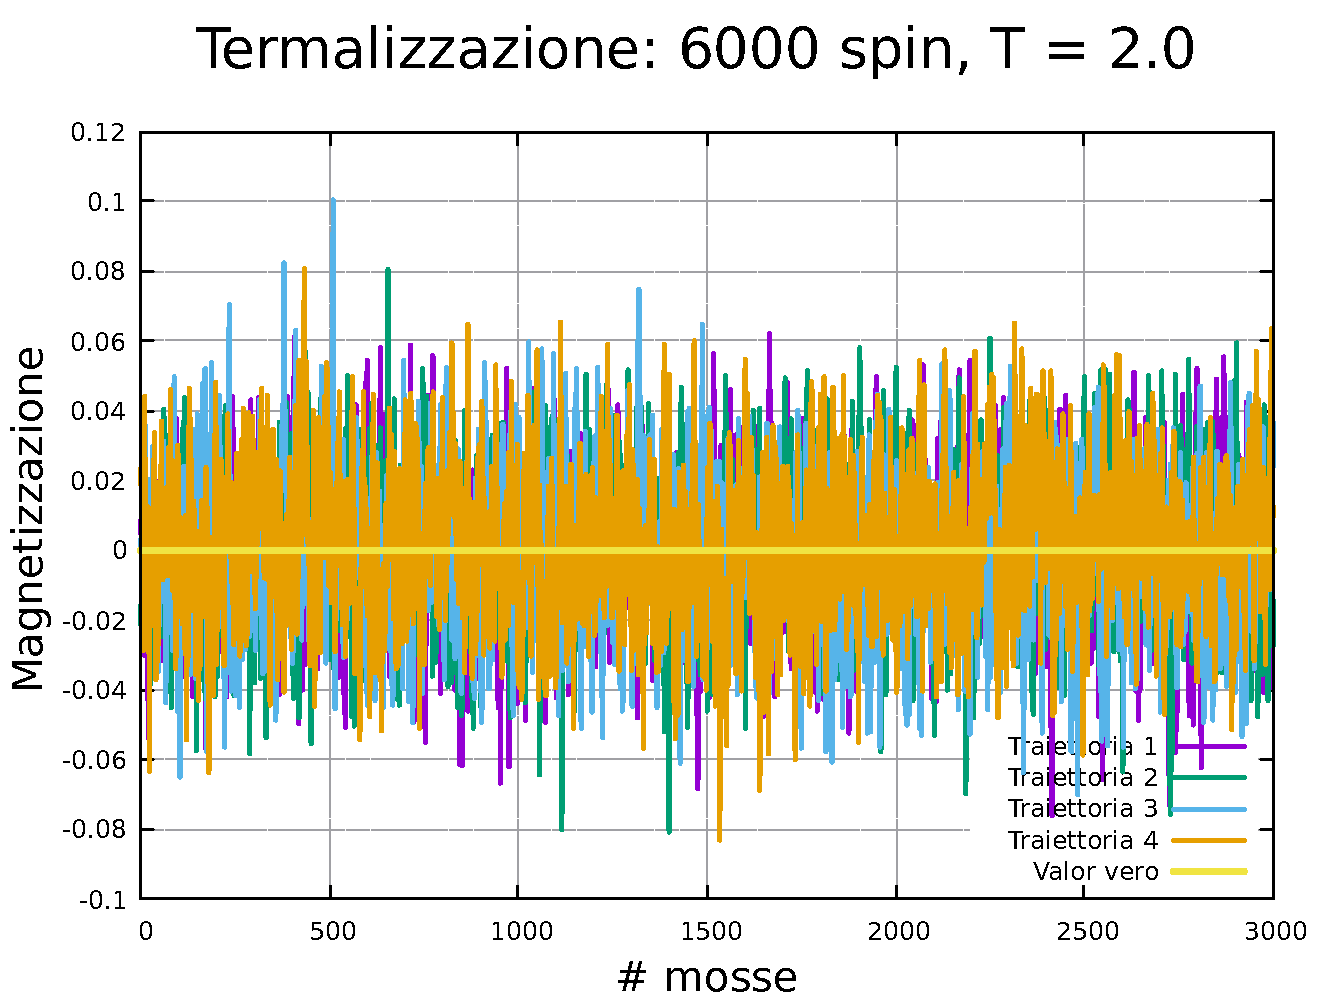
\includegraphics[page=1, width=\textwidth]{Immagini/simIsing1D/magn0.0/term/term_6000_2.0.pdf}
      \caption{$T\,=\,2.0$}
    \end{minipage}
    \caption{Studio della termalizzazione di un modello di Ising 1D costituito da 6000 spin.}
\end{figure}

\vspace*{\fill}

\newpage

\vspace*{\fill}

\begin{figure}[htbp]
    \centering
    \begin{minipage}{0.45\textwidth}  
      \centering
      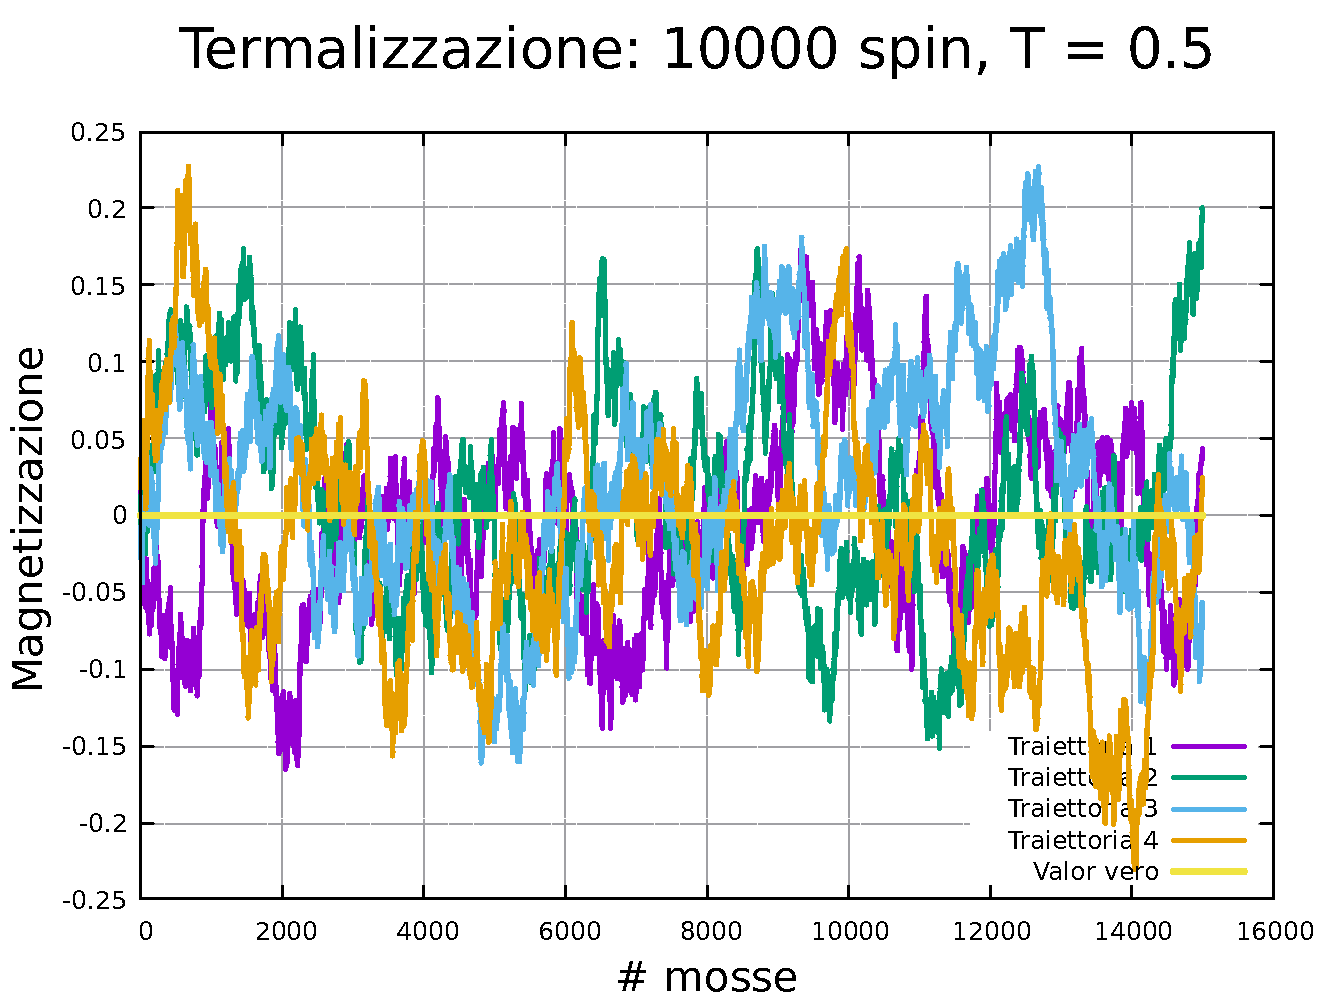
\includegraphics[page=1, width=\textwidth]{Immagini/simIsing1D/magn0.0/term/term_10000_0.5.pdf}
      \caption{$T\,=\,0.5$}
    \end{minipage}\hfill
    \begin{minipage}{0.45\textwidth}  
      \centering
      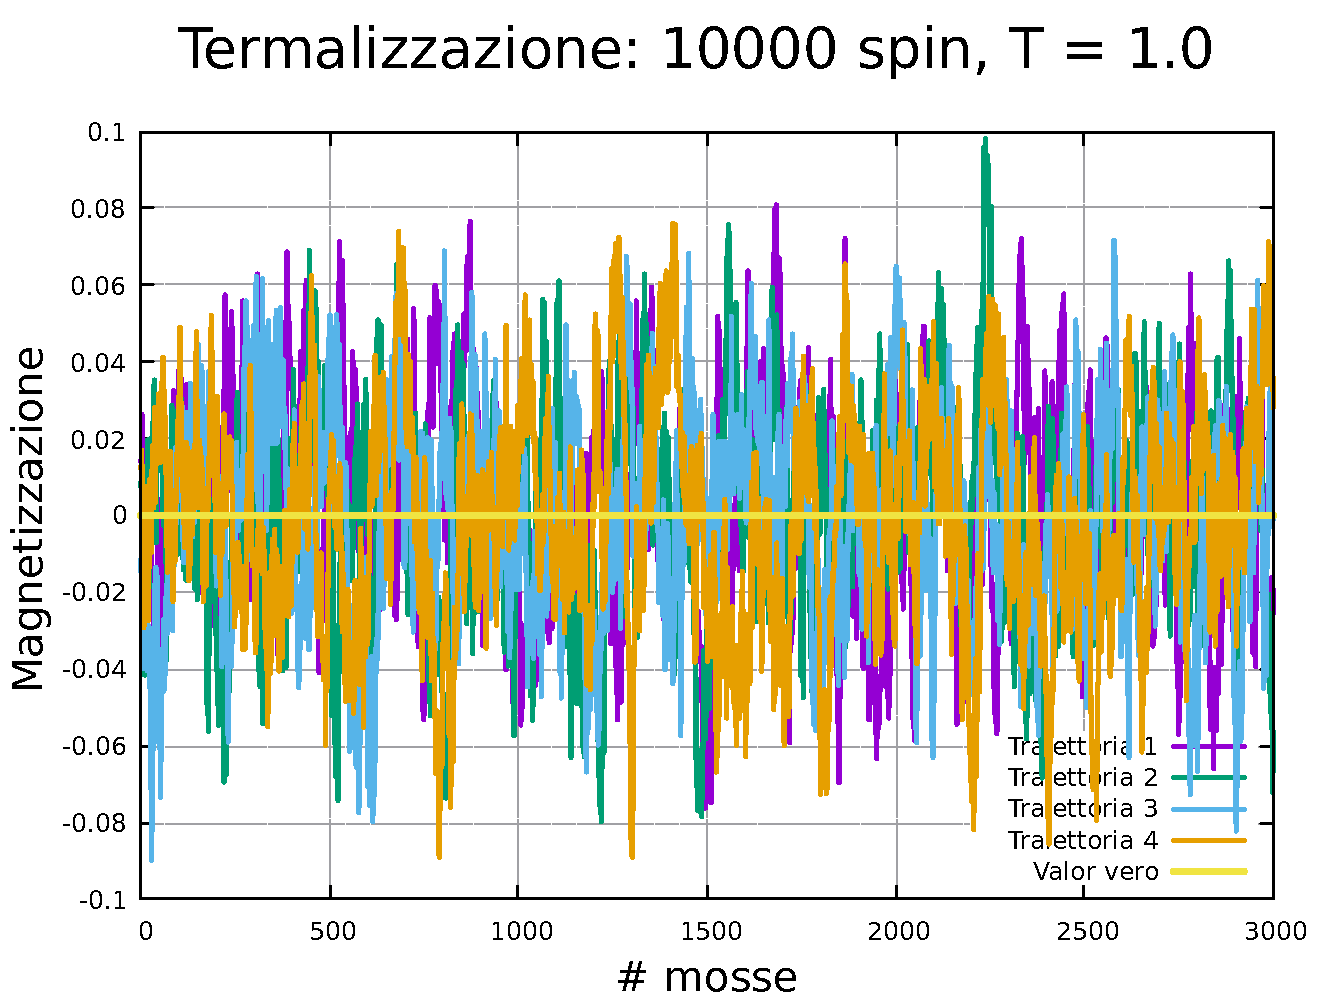
\includegraphics[page=1, width=\textwidth]{Immagini/simIsing1D/magn0.0/term/term_10000_1.0.pdf}
      \caption{$T\,=\,1.0$}
    \end{minipage}
    \vskip\baselineskip 
  
    \begin{minipage}{0.45\textwidth}  
      \centering
      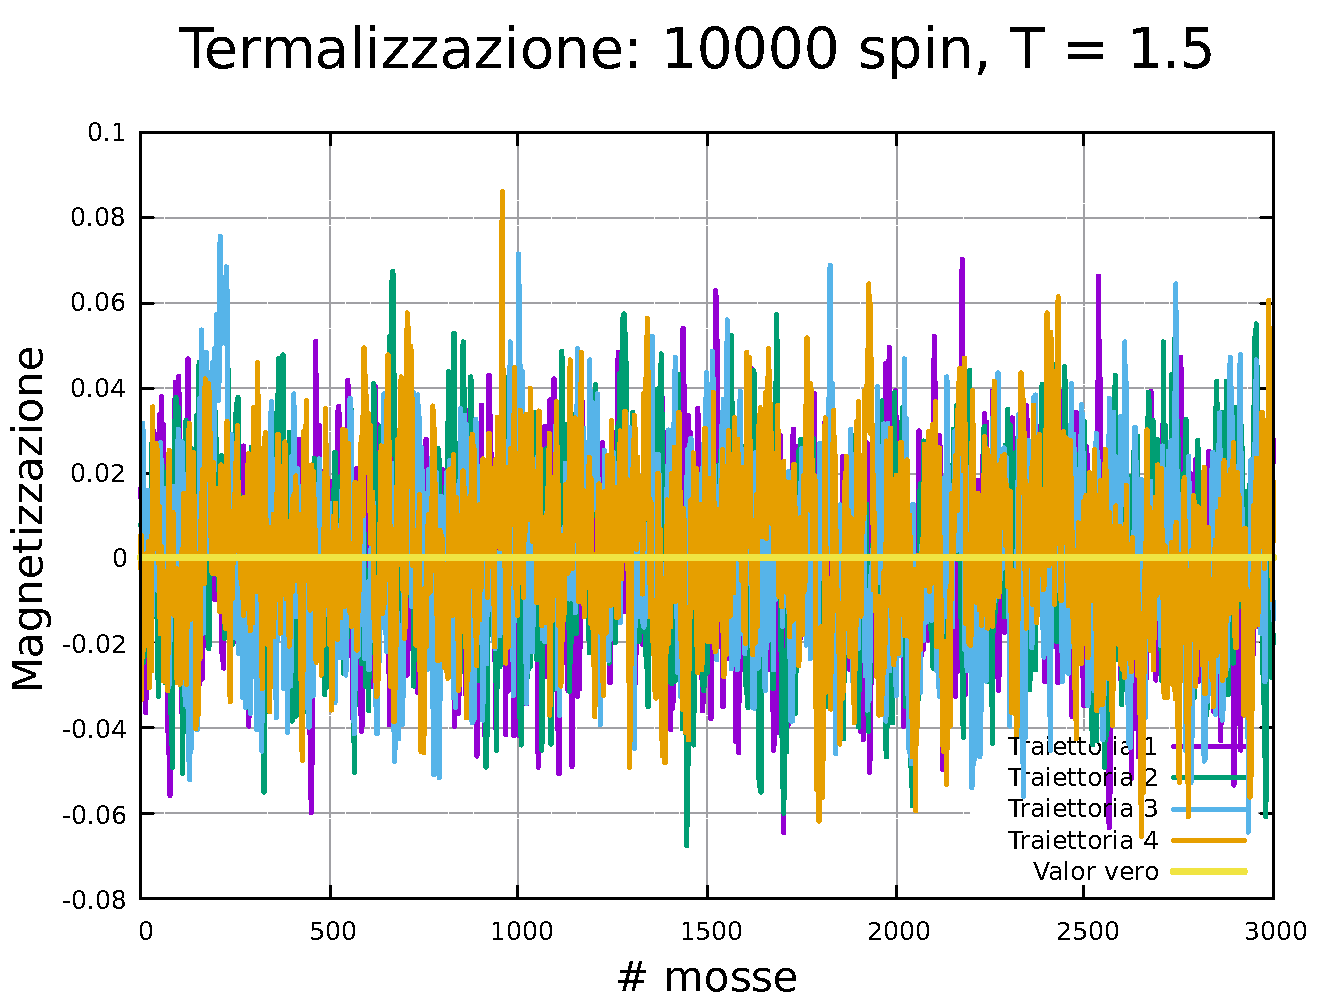
\includegraphics[page=1, width=\textwidth]{Immagini/simIsing1D/magn0.0/term/term_10000_1.5.pdf}
      \caption{$T\,=\,1.5$}
    \end{minipage}\hfill
    \begin{minipage}{0.45\textwidth}  
      \centering
      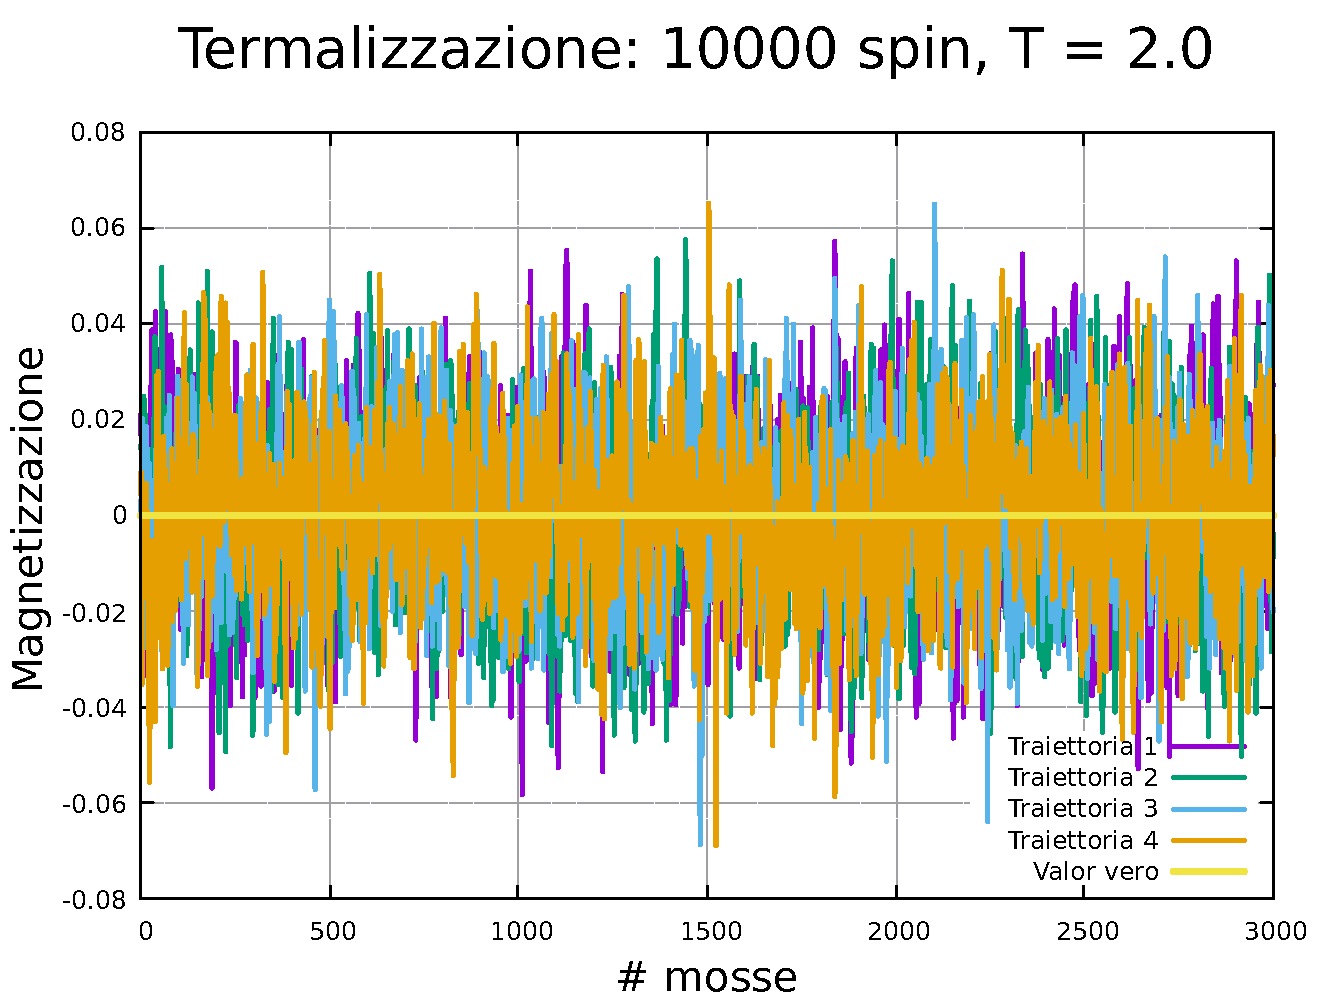
\includegraphics[page=1, width=\textwidth]{Immagini/simIsing1D/magn0.0/term/term_10000_2.0.pdf}
      \caption{$T\,=\,2.0$}
    \end{minipage}
    \caption{Studio della termalizzazione di un modello di Ising 1D costituito da 10000 spin.}
\end{figure}

\vspace*{\fill}

\newpage



\subsection{Auto-correlazione}

\vspace*{\fill}

\begin{figure}[htbp]
    \centering
    \begin{minipage}{0.45\textwidth}  
      \centering
      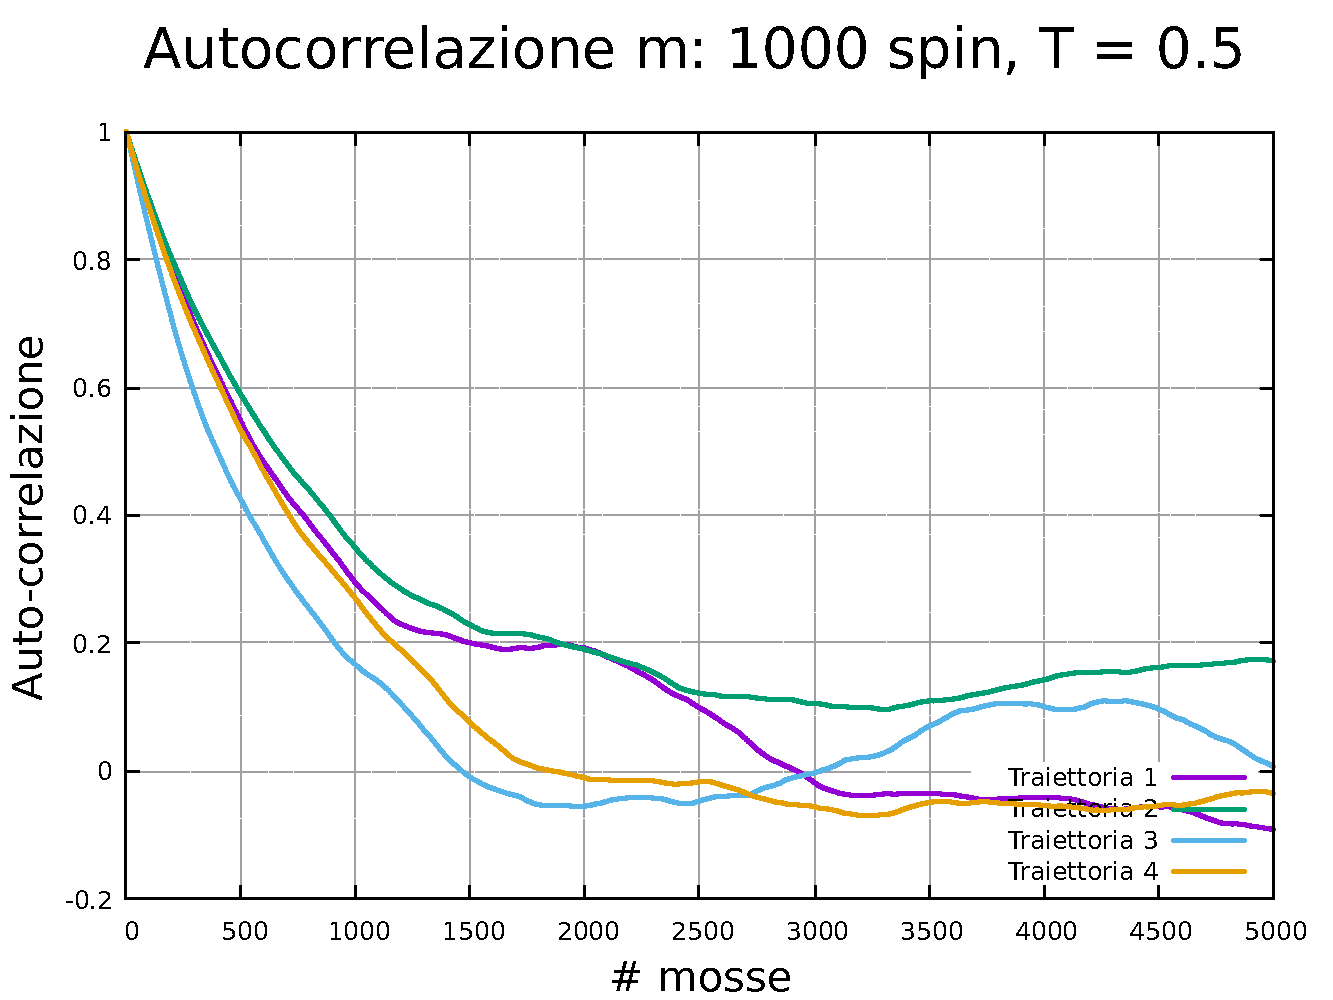
\includegraphics[page=1, width=\textwidth]{Immagini/simIsing1D/magn0.0/tcorr/auto_1000_0.5.pdf}
      \caption{$T\,=\,0.5$}
    \end{minipage}\hfill
    \begin{minipage}{0.45\textwidth}  
      \centering
      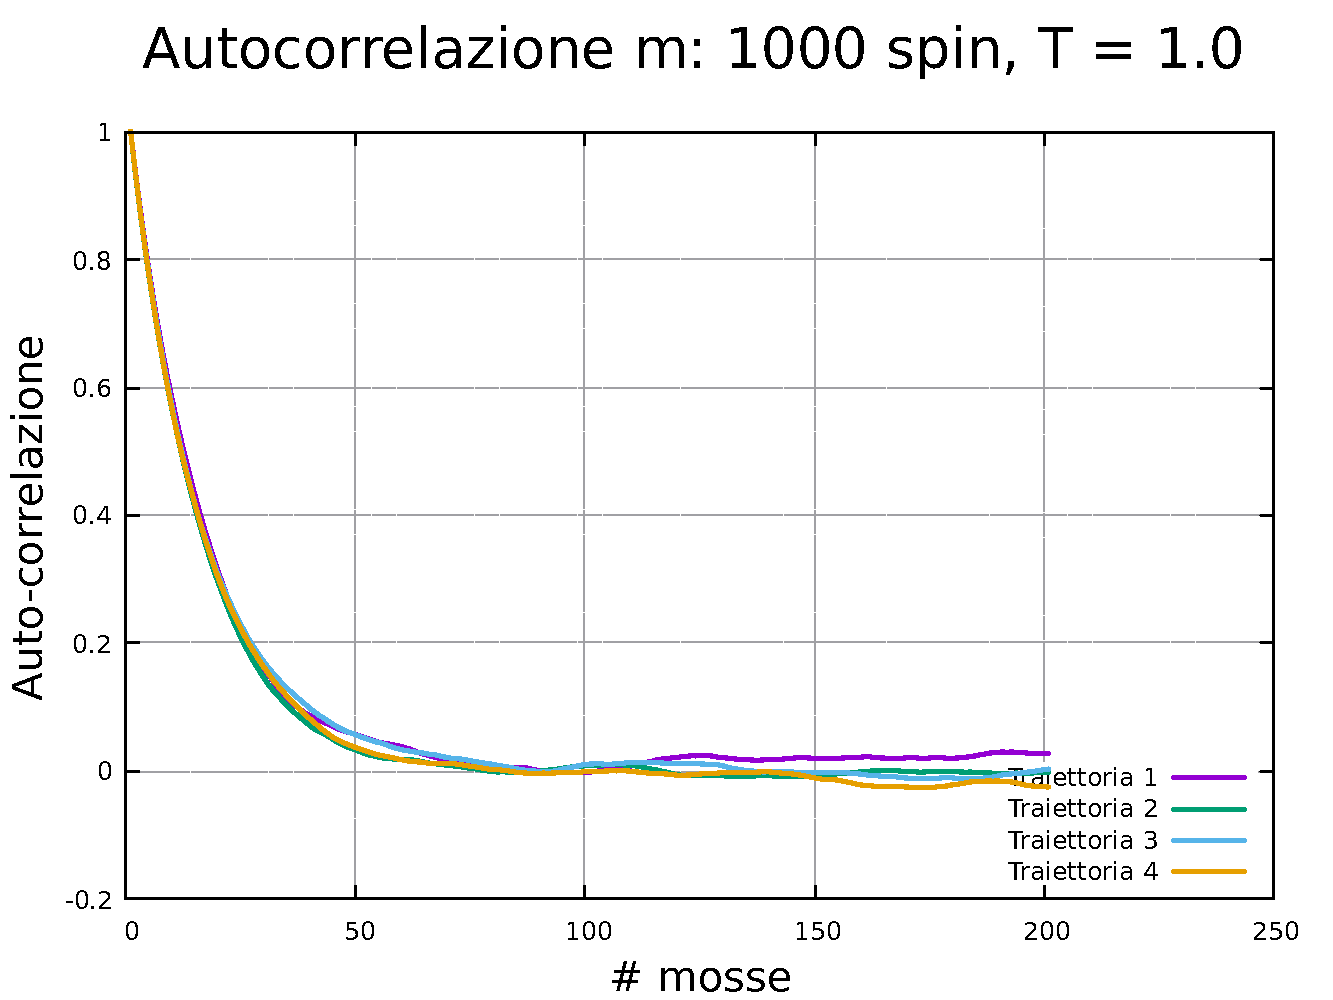
\includegraphics[page=1, width=\textwidth]{Immagini/simIsing1D/magn0.0/tcorr/auto_1000_1.0.pdf}
      \caption{$T\,=\,1.0$}
    \end{minipage}
    \vskip\baselineskip 
  
    \begin{minipage}{0.45\textwidth}  
      \centering
      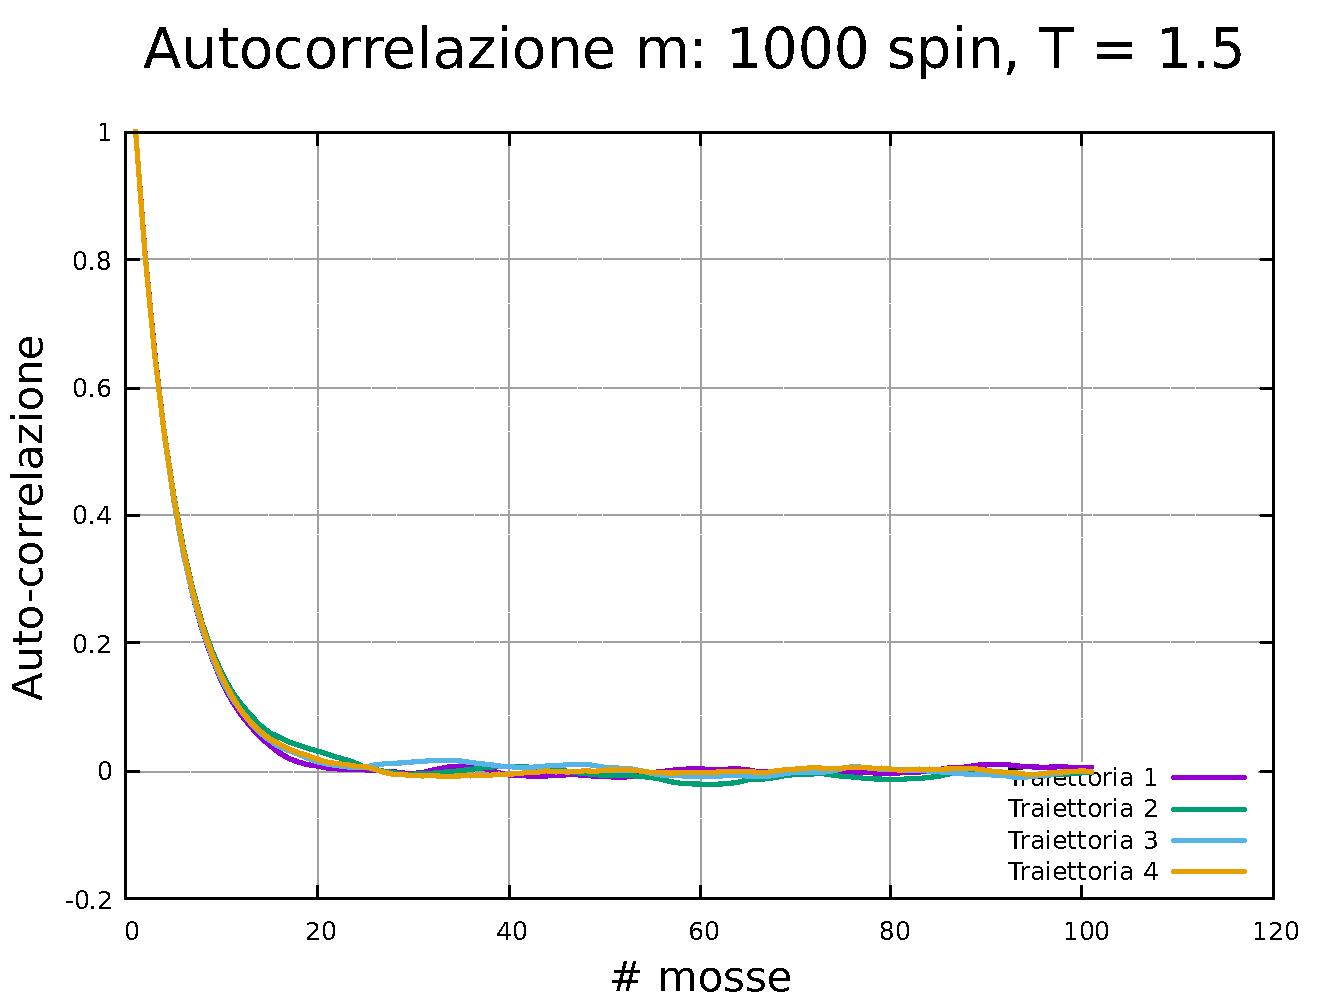
\includegraphics[page=1, width=\textwidth]{Immagini/simIsing1D/magn0.0/tcorr/auto_1000_1.5.pdf}
      \caption{$T\,=\,1.5$}
    \end{minipage}\hfill
    \begin{minipage}{0.45\textwidth}  
      \centering
      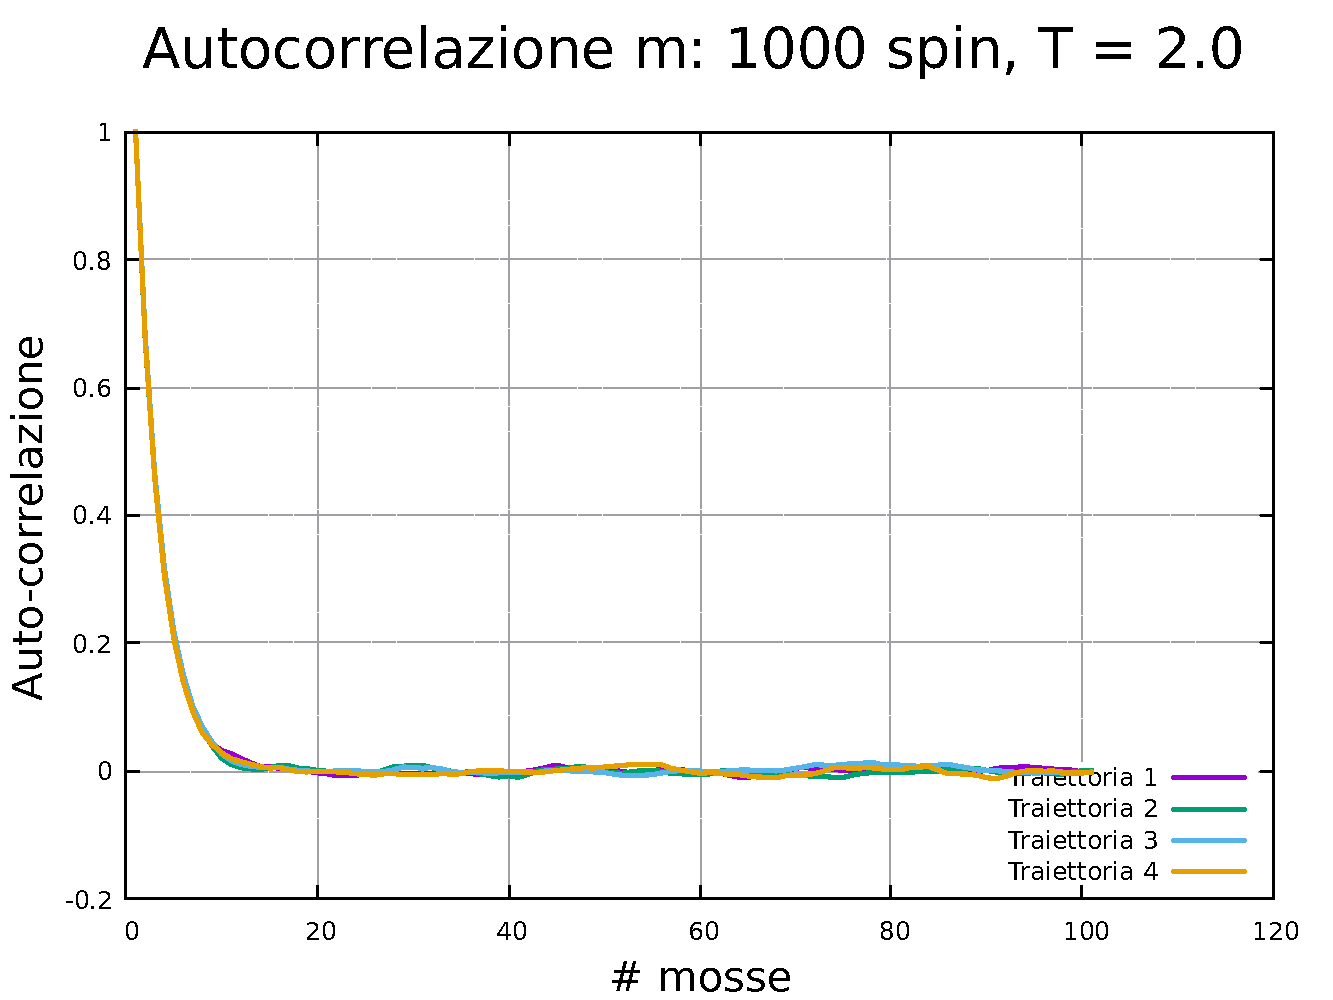
\includegraphics[page=1, width=\textwidth]{Immagini/simIsing1D/magn0.0/tcorr/auto_1000_2.0.pdf}
      \caption{$T\,=\,2.0$}
    \end{minipage}
    \caption{Studio dell'auto-correlazione per un modello di Ising 1D costituito da 1000 spin.}
\end{figure}

\vspace*{\fill}

\newpage

\vspace*{\fill}

\begin{figure}[htbp]
    \centering
    \begin{minipage}{0.45\textwidth}  
      \centering
      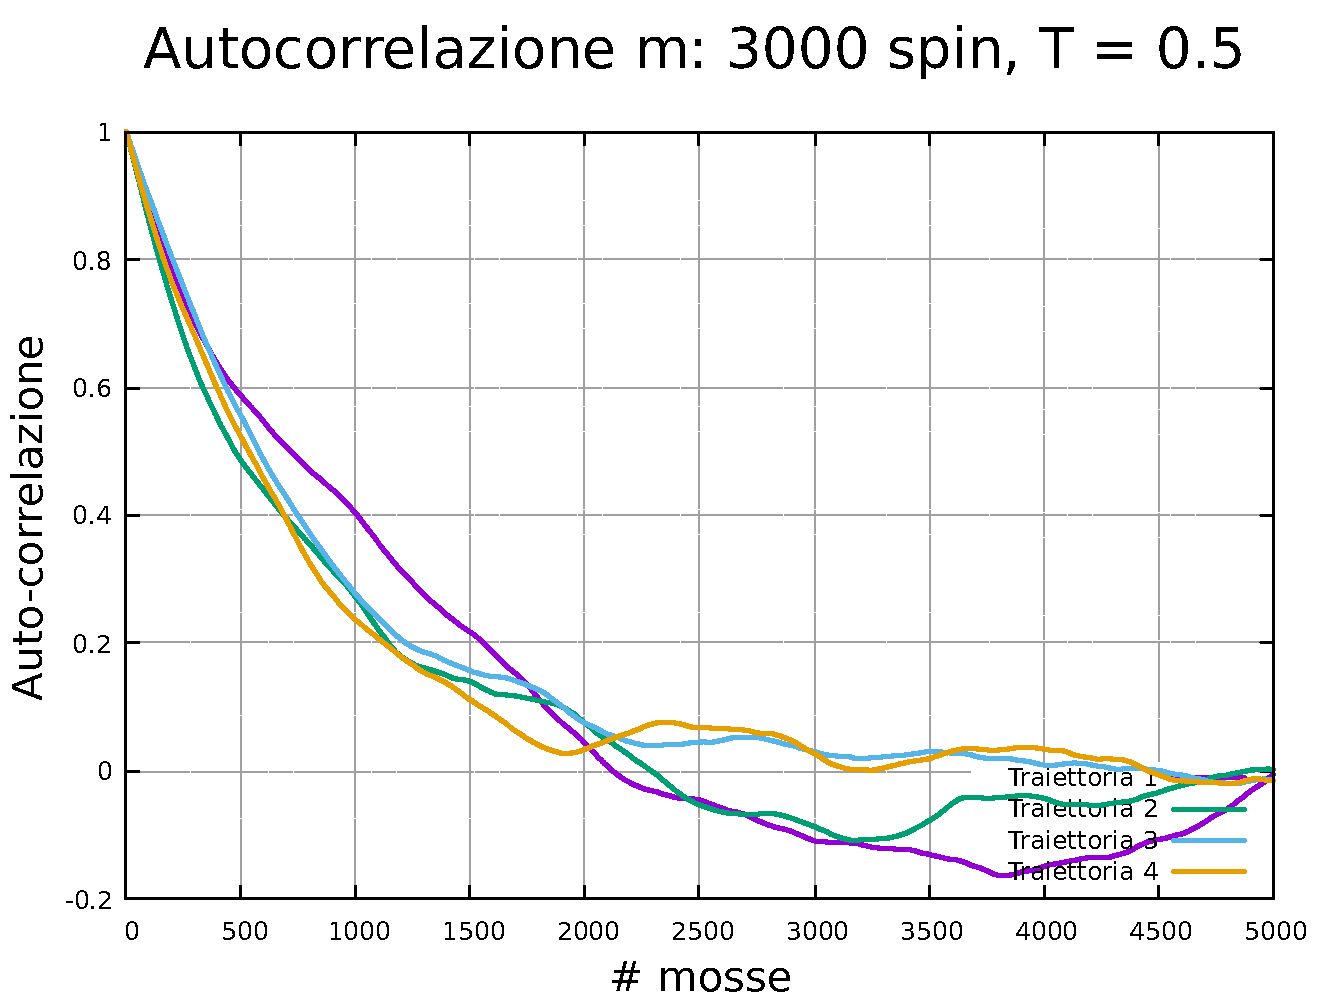
\includegraphics[page=1, width=\textwidth]{Immagini/simIsing1D/magn0.0/tcorr/auto_3000_0.5.pdf}
      \caption{$T\,=\,0.5$}
    \end{minipage}\hfill
    \begin{minipage}{0.45\textwidth}  
      \centering
      \includegraphics[page=1, width=\textwidth]{Immagini/simIsing1D/magn0.0/tcorr/auto_3000_1.0.pdf}
      \caption{$T\,=\,1.0$}
    \end{minipage}
    \vskip\baselineskip 
  
    \begin{minipage}{0.45\textwidth}  
      \centering
      \includegraphics[page=1, width=\textwidth]{Immagini/simIsing1D/magn0.0/tcorr/auto_3000_1.5.pdf}
      \caption{$T\,=\,1.5$}
    \end{minipage}\hfill
    \begin{minipage}{0.45\textwidth}  
      \centering
      \includegraphics[page=1, width=\textwidth]{Immagini/simIsing1D/magn0.0/tcorr/auto_3000_2.0.pdf}
      \caption{$T\,=\,2.0$}
    \end{minipage}
    \caption{Studio dell'auto-correlazione per un modello di Ising 1D costituito da 3000 spin.}
\end{figure}

\vspace*{\fill}

\newpage

\vspace*{\fill}

\begin{figure}[htbp]
    \centering
    \begin{minipage}{0.45\textwidth}  
      \centering
      \includegraphics[page=1, width=\textwidth]{Immagini/simIsing1D/magn0.0/tcorr/auto_6000_0.5.pdf}
      \caption{$T\,=\,0.5$}
    \end{minipage}\hfill
    \begin{minipage}{0.45\textwidth}  
      \centering
      \includegraphics[page=1, width=\textwidth]{Immagini/simIsing1D/magn0.0/tcorr/auto_6000_1.0.pdf}
      \caption{$T\,=\,1.0$}
    \end{minipage}
    \vskip\baselineskip 
  
    \begin{minipage}{0.45\textwidth}  
      \centering
      \includegraphics[page=1, width=\textwidth]{Immagini/simIsing1D/magn0.0/tcorr/auto_6000_1.5.pdf}
      \caption{$T\,=\,1.5$}
    \end{minipage}\hfill
    \begin{minipage}{0.45\textwidth}  
      \centering
      \includegraphics[page=1, width=\textwidth]{Immagini/simIsing1D/magn0.0/tcorr/auto_6000_2.0.pdf}
      \caption{$T\,=\,2.0$}
    \end{minipage}
    \caption{Studio dell'auto-correlazione per un modello di Ising 1D costituito da 6000 spin.}
\end{figure}

\vspace*{\fill}

\newpage

\vspace*{\fill}

\begin{figure}[htbp]
    \centering
    \begin{minipage}{0.45\textwidth}  
      \centering
      \includegraphics[page=1, width=\textwidth]{Immagini/simIsing1D/magn0.0/tcorr/auto_10000_0.5.pdf}
      \caption{$T\,=\,0.5$}
    \end{minipage}\hfill
    \begin{minipage}{0.45\textwidth}  
      \centering
      \includegraphics[page=1, width=\textwidth]{Immagini/simIsing1D/magn0.0/tcorr/auto_10000_1.0.pdf}
      \caption{$T\,=\,1.0$}
    \end{minipage}
    \vskip\baselineskip 
  
    \begin{minipage}{0.45\textwidth}  
      \centering
      \includegraphics[page=1, width=\textwidth]{Immagini/simIsing1D/magn0.0/tcorr/auto_10000_1.5.pdf}
      \caption{$T\,=\,1.5$}
    \end{minipage}\hfill
    \begin{minipage}{0.45\textwidth}  
      \centering
      \includegraphics[page=1, width=\textwidth]{Immagini/simIsing1D/magn0.0/tcorr/auto_10000_2.0.pdf}
      \caption{$T\,=\,2.0$}
    \end{minipage}
    \caption{Studio dell'auto-correlazione per un modello di Ising 1D costituito da 10000 spin.}
\end{figure}

\vspace*{\fill}

\newpage



\subsection{Dimensione dei blocchi}

\vspace*{\fill}

\begin{figure}[htbp]
    \centering
    \begin{minipage}{0.45\textwidth}  
      \centering
      \includegraphics[page=1, width=\textwidth]{Immagini/simIsing1D/magn0.0/lblk/err_1000_0.5.pdf}
      \caption{$T\,=\,0.5$}
    \end{minipage}\hfill
    \begin{minipage}{0.45\textwidth}  
      \centering
      \includegraphics[page=1, width=\textwidth]{Immagini/simIsing1D/magn0.0/lblk/err_1000_1.0.pdf}
      \caption{$T\,=\,1.0$}
    \end{minipage}
    \vskip\baselineskip 
  
    \begin{minipage}{0.45\textwidth}  
      \centering
      \includegraphics[page=1, width=\textwidth]{Immagini/simIsing1D/magn0.0/lblk/err_1000_1.5.pdf}
      \caption{$T\,=\,1.5$}
    \end{minipage}\hfill
    \begin{minipage}{0.45\textwidth}  
      \centering
      \includegraphics[page=1, width=\textwidth]{Immagini/simIsing1D/magn0.0/lblk/err_1000_2.0.pdf}
      \caption{$T\,=\,2.0$}
    \end{minipage}
    \caption{Errore in funzione della lunghezza dei blocchi per un modello di Ising 1D costituito da 1000 spin.}
\end{figure}

\vspace*{\fill}

\newpage

\vspace*{\fill}

\begin{figure}[htbp]
    \centering
    \begin{minipage}{0.45\textwidth}  
      \centering
      \includegraphics[page=1, width=\textwidth]{Immagini/simIsing1D/magn0.0/lblk/err_3000_0.5.pdf}
      \caption{$T\,=\,0.5$}
    \end{minipage}\hfill
    \begin{minipage}{0.45\textwidth}  
      \centering
      \includegraphics[page=1, width=\textwidth]{Immagini/simIsing1D/magn0.0/lblk/err_3000_1.0.pdf}
      \caption{$T\,=\,1.0$}
    \end{minipage}
    \vskip\baselineskip 
  
    \begin{minipage}{0.45\textwidth}  
      \centering
      \includegraphics[page=1, width=\textwidth]{Immagini/simIsing1D/magn0.0/lblk/err_3000_1.5.pdf}
      \caption{$T\,=\,1.5$}
    \end{minipage}\hfill
    \begin{minipage}{0.45\textwidth}  
      \centering
      \includegraphics[page=1, width=\textwidth]{Immagini/simIsing1D/magn0.0/lblk/err_3000_2.0.pdf}
      \caption{$T\,=\,2.0$}
    \end{minipage}
    \caption{Errore in funzione della lunghezza dei blocchi per un modello di Ising 1D costituito da 3000 spin.}
\end{figure}

\vspace*{\fill}

\newpage

\vspace*{\fill}

\begin{figure}[htbp]
    \centering
    \begin{minipage}{0.45\textwidth}  
      \centering
      \includegraphics[page=1, width=\textwidth]{Immagini/simIsing1D/magn0.0/lblk/err_6000_0.5.pdf}
      \caption{$T\,=\,0.5$}
    \end{minipage}\hfill
    \begin{minipage}{0.45\textwidth}  
      \centering
      \includegraphics[page=1, width=\textwidth]{Immagini/simIsing1D/magn0.0/lblk/err_6000_1.0.pdf}
      \caption{$T\,=\,1.0$}
    \end{minipage}
    \vskip\baselineskip 
  
    \begin{minipage}{0.45\textwidth}  
      \centering
      \includegraphics[page=1, width=\textwidth]{Immagini/simIsing1D/magn0.0/lblk/err_6000_1.5.pdf}
      \caption{$T\,=\,1.5$}
    \end{minipage}\hfill
    \begin{minipage}{0.45\textwidth}  
      \centering
      \includegraphics[page=1, width=\textwidth]{Immagini/simIsing1D/magn0.0/lblk/err_6000_2.0.pdf}
      \caption{$T\,=\,2.0$}
    \end{minipage}
    \caption{Errore in funzione della lunghezza dei blocchi per un modello di Ising 1D costituito da 6000 spin.}
\end{figure}

\vspace*{\fill}

\newpage

\vspace*{\fill}

\begin{figure}[htbp]
    \centering
    \begin{minipage}{0.45\textwidth}  
      \centering
      \includegraphics[page=1, width=\textwidth]{Immagini/simIsing1D/magn0.0/lblk/err_10000_0.5.pdf}
      \caption{$T\,=\,0.5$}
    \end{minipage}\hfill
    \begin{minipage}{0.45\textwidth}  
      \centering
      \includegraphics[page=1, width=\textwidth]{Immagini/simIsing1D/magn0.0/lblk/err_10000_1.0.pdf}
      \caption{$T\,=\,1.0$}
    \end{minipage}
    \vskip\baselineskip 
  
    \begin{minipage}{0.45\textwidth}  
      \centering
      \includegraphics[page=1, width=\textwidth]{Immagini/simIsing1D/magn0.0/lblk/err_10000_1.5.pdf}
      \caption{$T\,=\,1.5$}
    \end{minipage}\hfill
    \begin{minipage}{0.45\textwidth}  
      \centering
      \includegraphics[page=1, width=\textwidth]{Immagini/simIsing1D/magn0.0/lblk/err_10000_2.0.pdf}
      \caption{$T\,=\,2.0$}
    \end{minipage}
    \caption{Errore in funzione della lunghezza dei blocchi per un modello di Ising 1D costituito da 10000 spin.}
\end{figure}

\vspace*{\fill}

\newpage



\subsection{Osservabili}

\vspace*{\fill}

\begin{figure}[htbp]
    \centering
    \includegraphics[page=1, width=\textwidth]{Immagini/simIsing1D/obs/obs_1000_0.0.png}
    \caption{Osservabili di un modello di Ising 1D costituito da 1000 spin al variare di T.}
\end{figure}

\vspace*{\fill}

\newpage

\vspace*{\fill}

\begin{figure}[htbp]
    \centering
    \includegraphics[page=1, width=\textwidth]{Immagini/simIsing1D/obs/obs_1000_0.0_diff.png}
    \caption{Differenza dal valor vero per un modello di Ising 1D costituito da 1000 spin al variare di T.}
\end{figure}

\vspace*{\fill}

\newpage

\vspace*{\fill}

\begin{figure}[htbp]
    \centering
    \includegraphics[page=1, width=\textwidth]{Immagini/simIsing1D/obs/obs_3000_0.0.png}
    \caption{Osservabili di un modello di Ising 1D costituito da 3000 spin al variare di T.}
\end{figure}

\vspace*{\fill}

\newpage

\vspace*{\fill}

\begin{figure}[htbp]
    \centering
    \includegraphics[page=1, width=\textwidth]{Immagini/simIsing1D/obs/obs_3000_0.0_diff.png}
    \caption{Differenza dal valor vero per un modello di Ising 1D costituito da 3000 spin al variare di T.}
\end{figure}

\vspace*{\fill}

\newpage

\vspace*{\fill}

\begin{figure}[htbp]
    \centering
    \includegraphics[page=1, width=\textwidth]{Immagini/simIsing1D/obs/obs_6000_0.0.png}
    \caption{Osservabili di un modello di Ising 1D costituito da 6000 spin al variare di T.}
\end{figure}

\vspace*{\fill}

\newpage

\vspace*{\fill}

\begin{figure}[htbp]
    \centering
    \includegraphics[page=1, width=\textwidth]{Immagini/simIsing1D/obs/obs_6000_0.0_diff.png}
    \caption{Differenza dal valor vero per un modello di Ising 1D costituito da 6000 spin al variare di T.}
\end{figure}

\vspace*{\fill}

\newpage

% \vspace*{\fill}
% 
% \begin{figure}[htbp]
%     \centering
%     \includegraphics[page=1, width=\textwidth]{Immagini/simIsing1D/obs/obs_10000_0.0.png}
%     \caption{Osservabili di un modello di Ising 1D costituito da 10000 spin al variare di T.}
% \end{figure}
% 
% \vspace*{\fill}
% 
% \newpage
% 
% \vspace*{\fill}
% 
% \begin{figure}[htbp]
%     \centering
%     \includegraphics[page=1, width=\textwidth]{Immagini/simIsing1D/obs/obs_10000_0.0_diff.png}
%     \caption{Differenza dal valor vero per un modello di Ising 1D costituito da 10000 spin al variare di T.}
% \end{figure}
% 
% \vspace*{\fill}
% 
% \newpage

\section{Modello di Ising 1D: $h\,=\,0.02$}
\subsection{Simulazioni con campo magnetico $h\,=\,0.02$}

La prima fase della simulazione del modello di Ising 1D è incentrata sulla determinazione dei parametri ottimali per ottenere 
dei valori d'aspettazione statisticamente rilevanti, in modo tale da poter effettuare il confronto con il valor vero noto in letteratura. In 
questa fase preliminare ho lavorato con le seguenti quattro lunghezze del modello di Ising 1D e le seguenti quattro temperature 

\begin{equation}
    l\,\in\,\left\{1000,\,3000,\,6000,\,10000\right\}
    \label{eq: dim_sim_Ising1D}
\end{equation}

\begin{equation}
    T\,\in\,\left\{0.5,\,1.0,\,1.5,\,2.0\right\}
    \label{eq: temp_sim_Ising1D}
\end{equation}

Per ognuna di queste coppie dimensione-temperatura ho considerato quattro seed differenti del generatore di numeri casuali in modo da 
poter analizzare il comportamento del sistema lungo differenti traiettorie nello spazio delle fasi. 



\subsubsection{Termalizzazione}

La lunghezza della fase di termalizzazione dipende fortemente dal valore della temperatura a cui viene svolta la simulazione, come è 
possibile osservare nelle seguenti Figure in cui sono riportati i risultati ottenuti raggruppati per lunghezza della catena di spin. 
La durata maggiore della termalizzazione si ha per la temperatura inferiore, ossia $T\,=\,0.5$, poichè per giungere ad una configurazione 
ordinata (come evidente dal valore della magnetizzazione tendente ad uno) è necessario un tempo computazionale maggiore legato alla 
necessità di orientare tutti gli spin in modo concorde.

\newpage

\vspace*{\fill}

\begin{figure}[htbp]
    \centering
    \begin{minipage}{0.45\textwidth}  
      \centering
      \includegraphics[page=1, width=\textwidth]{Immagini/simIsing1D/magn0.02/term/term_1000_0.5.pdf}
      \caption{$T\,=\,0.5$}
    \end{minipage}\hfill
    \begin{minipage}{0.45\textwidth}  
      \centering
      \includegraphics[page=1, width=\textwidth]{Immagini/simIsing1D/magn0.02/term/term_1000_1.0.pdf}
      \caption{$T\,=\,1.0$}
    \end{minipage}
    \vskip\baselineskip 
  
    \begin{minipage}{0.45\textwidth}  
      \centering
      \includegraphics[page=1, width=\textwidth]{Immagini/simIsing1D/magn0.02/term/term_1000_1.5.pdf}
      \caption{$T\,=\,1.5$}
    \end{minipage}\hfill
    \begin{minipage}{0.45\textwidth}  
      \centering
      \includegraphics[page=1, width=\textwidth]{Immagini/simIsing1D/magn0.02/term/term_1000_2.0.pdf}
      \caption{$T\,=\,2.0$}
    \end{minipage}
    \caption{Studio della termalizzazione di un modello di Ising 1D costituito da 1000 spin.}
\end{figure}

\vspace*{\fill}

\newpage

\vspace*{\fill}

\begin{figure}[htbp]
    \centering
    \begin{minipage}{0.45\textwidth}  
      \centering
      \includegraphics[page=1, width=\textwidth]{Immagini/simIsing1D/magn0.02/term/term_3000_0.5.pdf}
      \caption{$T\,=\,0.5$}
    \end{minipage}\hfill
    \begin{minipage}{0.45\textwidth}  
      \centering
      \includegraphics[page=1, width=\textwidth]{Immagini/simIsing1D/magn0.02/term/term_3000_1.0.pdf}
      \caption{$T\,=\,1.0$}
    \end{minipage}
    \vskip\baselineskip 
  
    \begin{minipage}{0.45\textwidth}  
      \centering
      \includegraphics[page=1, width=\textwidth]{Immagini/simIsing1D/magn0.02/term/term_3000_1.5.pdf}
      \caption{$T\,=\,1.5$}
    \end{minipage}\hfill
    \begin{minipage}{0.45\textwidth}  
      \centering
      \includegraphics[page=1, width=\textwidth]{Immagini/simIsing1D/magn0.02/term/term_3000_2.0.pdf}
      \caption{$T\,=\,2.0$}
    \end{minipage}
    \caption{Studio della termalizzazione di un modello di Ising 1D costituito da 3000 spin.}
\end{figure}

\vspace*{\fill}

\newpage

\vspace*{\fill}

\begin{figure}[htbp]
    \centering
    \begin{minipage}{0.45\textwidth}  
      \centering
      \includegraphics[page=1, width=\textwidth]{Immagini/simIsing1D/magn0.02/term/term_6000_0.5.pdf}
      \caption{$T\,=\,0.5$}
    \end{minipage}\hfill
    \begin{minipage}{0.45\textwidth}  
      \centering
      \includegraphics[page=1, width=\textwidth]{Immagini/simIsing1D/magn0.02/term/term_6000_1.0.pdf}
      \caption{$T\,=\,1.0$}
    \end{minipage}
    \vskip\baselineskip 
  
    \begin{minipage}{0.45\textwidth}  
      \centering
      \includegraphics[page=1, width=\textwidth]{Immagini/simIsing1D/magn0.02/term/term_6000_1.5.pdf}
      \caption{$T\,=\,1.5$}
    \end{minipage}\hfill
    \begin{minipage}{0.45\textwidth}  
      \centering
      \includegraphics[page=1, width=\textwidth]{Immagini/simIsing1D/magn0.02/term/term_6000_2.0.pdf}
      \caption{$T\,=\,2.0$}
    \end{minipage}
    \caption{Studio della termalizzazione di un modello di Ising 1D costituito da 6000 spin.}
\end{figure}

\vspace*{\fill}

\newpage

\vspace*{\fill}

\begin{figure}[htbp]
    \centering
    \begin{minipage}{0.45\textwidth}  
      \centering
      \includegraphics[page=1, width=\textwidth]{Immagini/simIsing1D/magn0.02/term/term_10000_0.5.pdf}
      \caption{$T\,=\,0.5$}
    \end{minipage}\hfill
    \begin{minipage}{0.45\textwidth}  
      \centering
      \includegraphics[page=1, width=\textwidth]{Immagini/simIsing1D/magn0.02/term/term_10000_1.0.pdf}
      \caption{$T\,=\,1.0$}
    \end{minipage}
    \vskip\baselineskip 
  
    \begin{minipage}{0.45\textwidth}  
      \centering
      \includegraphics[page=1, width=\textwidth]{Immagini/simIsing1D/magn0.02/term/term_10000_1.5.pdf}
      \caption{$T\,=\,1.5$}
    \end{minipage}\hfill
    \begin{minipage}{0.45\textwidth}  
      \centering
      \includegraphics[page=1, width=\textwidth]{Immagini/simIsing1D/magn0.02/term/term_10000_2.0.pdf}
      \caption{$T\,=\,2.0$}
    \end{minipage}
    \caption{Studio della termalizzazione di un modello di Ising 1D costituito da 10000 spin.}
\end{figure}

\vspace*{\fill}

\newpage



\subsubsection{Auto-correlazione}

\vspace*{\fill}

\begin{figure}[htbp]
    \centering
    \begin{minipage}{0.45\textwidth}  
      \centering
      \includegraphics[page=1, width=\textwidth]{Immagini/simIsing1D/magn0.02/tcorr/tcorr_1000_0.5.pdf}
      \caption{$T\,=\,0.5$}
    \end{minipage}\hfill
    \begin{minipage}{0.45\textwidth}  
      \centering
      \includegraphics[page=1, width=\textwidth]{Immagini/simIsing1D/magn0.02/tcorr/tcorr_1000_1.0.pdf}
      \caption{$T\,=\,1.0$}
    \end{minipage}
    \vskip\baselineskip 
  
    \begin{minipage}{0.45\textwidth}  
      \centering
      \includegraphics[page=1, width=\textwidth]{Immagini/simIsing1D/magn0.02/tcorr/tcorr_1000_1.5.pdf}
      \caption{$T\,=\,1.5$}
    \end{minipage}\hfill
    \begin{minipage}{0.45\textwidth}  
      \centering
      \includegraphics[page=1, width=\textwidth]{Immagini/simIsing1D/magn0.02/tcorr/tcorr_1000_2.0.pdf}
      \caption{$T\,=\,2.0$}
    \end{minipage}
    \caption{Studio dell'auto-correlazione per un modello di Ising 1D costituito da 1000 spin.}
\end{figure}

\vspace*{\fill}

\newpage

\vspace*{\fill}

\begin{figure}[htbp]
    \centering
    \begin{minipage}{0.45\textwidth}  
      \centering
      \includegraphics[page=1, width=\textwidth]{Immagini/simIsing1D/magn0.02/tcorr/tcorr_3000_0.5.pdf}
      \caption{$T\,=\,0.5$}
    \end{minipage}\hfill
    \begin{minipage}{0.45\textwidth}  
      \centering
      \includegraphics[page=1, width=\textwidth]{Immagini/simIsing1D/magn0.02/tcorr/tcorr_3000_1.0.pdf}
      \caption{$T\,=\,1.0$}
    \end{minipage}
    \vskip\baselineskip 
  
    \begin{minipage}{0.45\textwidth}  
      \centering
      \includegraphics[page=1, width=\textwidth]{Immagini/simIsing1D/magn0.02/tcorr/tcorr_3000_1.5.pdf}
      \caption{$T\,=\,1.5$}
    \end{minipage}\hfill
    \begin{minipage}{0.45\textwidth}  
      \centering
      \includegraphics[page=1, width=\textwidth]{Immagini/simIsing1D/magn0.02/tcorr/tcorr_3000_2.0.pdf}
      \caption{$T\,=\,2.0$}
    \end{minipage}
    \caption{Studio dell'auto-correlazione per un modello di Ising 1D costituito da 3000 spin.}
\end{figure}

\vspace*{\fill}

\newpage

\vspace*{\fill}

\begin{figure}[htbp]
    \centering
    \begin{minipage}{0.45\textwidth}  
      \centering
      \includegraphics[page=1, width=\textwidth]{Immagini/simIsing1D/magn0.02/tcorr/tcorr_6000_0.5.pdf}
      \caption{$T\,=\,0.5$}
    \end{minipage}\hfill
    \begin{minipage}{0.45\textwidth}  
      \centering
      \includegraphics[page=1, width=\textwidth]{Immagini/simIsing1D/magn0.02/tcorr/tcorr_6000_1.0.pdf}
      \caption{$T\,=\,1.0$}
    \end{minipage}
    \vskip\baselineskip 
  
    \begin{minipage}{0.45\textwidth}  
      \centering
      \includegraphics[page=1, width=\textwidth]{Immagini/simIsing1D/magn0.02/tcorr/tcorr_6000_1.5.pdf}
      \caption{$T\,=\,1.5$}
    \end{minipage}\hfill
    \begin{minipage}{0.45\textwidth}  
      \centering
      \includegraphics[page=1, width=\textwidth]{Immagini/simIsing1D/magn0.02/tcorr/tcorr_6000_2.0.pdf}
      \caption{$T\,=\,2.0$}
    \end{minipage}
    \caption{Studio dell'auto-correlazione per un modello di Ising 1D costituito da 6000 spin.}
\end{figure}

\vspace*{\fill}

\newpage

\vspace*{\fill}

\begin{figure}[htbp]
    \centering
    \begin{minipage}{0.45\textwidth}  
      \centering
      \includegraphics[page=1, width=\textwidth]{Immagini/simIsing1D/magn0.02/tcorr/tcorr_10000_0.5.pdf}
      \caption{$T\,=\,0.5$}
    \end{minipage}\hfill
    \begin{minipage}{0.45\textwidth}  
      \centering
      \includegraphics[page=1, width=\textwidth]{Immagini/simIsing1D/magn0.02/tcorr/tcorr_10000_1.0.pdf}
      \caption{$T\,=\,1.0$}
    \end{minipage}
    \vskip\baselineskip 
  
    \begin{minipage}{0.45\textwidth}  
      \centering
      \includegraphics[page=1, width=\textwidth]{Immagini/simIsing1D/magn0.02/tcorr/tcorr_10000_1.5.pdf}
      \caption{$T\,=\,1.5$}
    \end{minipage}\hfill
    \begin{minipage}{0.45\textwidth}  
      \centering
      \includegraphics[page=1, width=\textwidth]{Immagini/simIsing1D/magn0.02/tcorr/tcorr_10000_2.0.pdf}
      \caption{$T\,=\,2.0$}
    \end{minipage}
    \caption{Studio dell'auto-correlazione per un modello di Ising 1D costituito da 10000 spin.}
\end{figure}

\vspace*{\fill}

\newpage



\subsubsection{Dimensione dei blocchi}

\vspace*{\fill}

\begin{figure}[htbp]
    \centering
    \begin{minipage}{0.45\textwidth}  
      \centering
      \includegraphics[page=1, width=\textwidth]{Immagini/simIsing1D/magn0.02/lblk/err_1000_0.5.pdf}
      \caption{$T\,=\,0.5$}
    \end{minipage}\hfill
    \begin{minipage}{0.45\textwidth}  
      \centering
      \includegraphics[page=1, width=\textwidth]{Immagini/simIsing1D/magn0.02/lblk/err_1000_1.0.pdf}
      \caption{$T\,=\,1.0$}
    \end{minipage}
    \vskip\baselineskip 
  
    \begin{minipage}{0.45\textwidth}  
      \centering
      \includegraphics[page=1, width=\textwidth]{Immagini/simIsing1D/magn0.02/lblk/err_1000_1.5.pdf}
      \caption{$T\,=\,1.5$}
    \end{minipage}\hfill
    \begin{minipage}{0.45\textwidth}  
      \centering
      \includegraphics[page=1, width=\textwidth]{Immagini/simIsing1D/magn0.02/lblk/err_1000_2.0.pdf}
      \caption{$T\,=\,2.0$}
    \end{minipage}
    \caption{Errore in funzione della lunghezza dei blocchi per un modello di Ising 1D costituito da 1000 spin.}
\end{figure}

\vspace*{\fill}

\newpage

\vspace*{\fill}

\begin{figure}[htbp]
    \centering
    \begin{minipage}{0.45\textwidth}  
      \centering
      \includegraphics[page=1, width=\textwidth]{Immagini/simIsing1D/magn0.02/lblk/err_3000_0.5.pdf}
      \caption{$T\,=\,0.5$}
    \end{minipage}\hfill
    \begin{minipage}{0.45\textwidth}  
      \centering
      \includegraphics[page=1, width=\textwidth]{Immagini/simIsing1D/magn0.02/lblk/err_3000_1.0.pdf}
      \caption{$T\,=\,1.0$}
    \end{minipage}
    \vskip\baselineskip 
  
    \begin{minipage}{0.45\textwidth}  
      \centering
      \includegraphics[page=1, width=\textwidth]{Immagini/simIsing1D/magn0.02/lblk/err_3000_1.5.pdf}
      \caption{$T\,=\,1.5$}
    \end{minipage}\hfill
    \begin{minipage}{0.45\textwidth}  
      \centering
      \includegraphics[page=1, width=\textwidth]{Immagini/simIsing1D/magn0.02/lblk/err_3000_2.0.pdf}
      \caption{$T\,=\,2.0$}
    \end{minipage}
    \caption{Errore in funzione della lunghezza dei blocchi per un modello di Ising 1D costituito da 3000 spin.}
\end{figure}

\vspace*{\fill}

\newpage

\vspace*{\fill}

\begin{figure}[htbp]
    \centering
    \begin{minipage}{0.45\textwidth}  
      \centering
      \includegraphics[page=1, width=\textwidth]{Immagini/simIsing1D/magn0.02/lblk/err_6000_0.5.pdf}
      \caption{$T\,=\,0.5$}
    \end{minipage}\hfill
    \begin{minipage}{0.45\textwidth}  
      \centering
      \includegraphics[page=1, width=\textwidth]{Immagini/simIsing1D/magn0.02/lblk/err_6000_1.0.pdf}
      \caption{$T\,=\,1.0$}
    \end{minipage}
    \vskip\baselineskip 
  
    \begin{minipage}{0.45\textwidth}  
      \centering
      \includegraphics[page=1, width=\textwidth]{Immagini/simIsing1D/magn0.02/lblk/err_6000_1.5.pdf}
      \caption{$T\,=\,1.5$}
    \end{minipage}\hfill
    \begin{minipage}{0.45\textwidth}  
      \centering
      \includegraphics[page=1, width=\textwidth]{Immagini/simIsing1D/magn0.02/lblk/err_6000_2.0.pdf}
      \caption{$T\,=\,2.0$}
    \end{minipage}
    \caption{Errore in funzione della lunghezza dei blocchi per un modello di Ising 1D costituito da 6000 spin.}
\end{figure}

\vspace*{\fill}

\newpage

\vspace*{\fill}

\begin{figure}[htbp]
    \centering
    \begin{minipage}{0.45\textwidth}  
      \centering
      \includegraphics[page=1, width=\textwidth]{Immagini/simIsing1D/magn0.02/lblk/err_10000_0.5.pdf}
      \caption{$T\,=\,0.5$}
    \end{minipage}\hfill
    \begin{minipage}{0.45\textwidth}  
      \centering
      \includegraphics[page=1, width=\textwidth]{Immagini/simIsing1D/magn0.02/lblk/err_10000_1.0.pdf}
      \caption{$T\,=\,1.0$}
    \end{minipage}
    \vskip\baselineskip 
  
    \begin{minipage}{0.45\textwidth}  
      \centering
      \includegraphics[page=1, width=\textwidth]{Immagini/simIsing1D/magn0.02/lblk/err_10000_1.5.pdf}
      \caption{$T\,=\,1.5$}
    \end{minipage}\hfill
    \begin{minipage}{0.45\textwidth}  
      \centering
      \includegraphics[page=1, width=\textwidth]{Immagini/simIsing1D/magn0.02/lblk/err_10000_2.0.pdf}
      \caption{$T\,=\,2.0$}
    \end{minipage}
    \caption{Errore in funzione della lunghezza dei blocchi per un modello di Ising 1D costituito da 10000 spin.}
\end{figure}

\vspace*{\fill}

\newpage




%-------------------------------------------%
%          Modello di Ising 2D              %
%-------------------------------------------%
\section{Modello di Ising 2D: Metropolis}
\subsection{Simulazioni con algoritmo di Metropolis}

Le simulazioni considerate in questa sottosezione sono state effettuate con l'algoritmo di Metropolis, la cui 
implementazione è riportata in seguito. Per ogni mossa Monte-Carlo, viene tentato un numero di singole inversioni degli spin 
pari al numero di siti reticolari del modello stesso.

\begin{minted}[frame=lines, fontsize=\small, bgcolor=blue!10, breaklines = true]{nim}
  proc metropolisMove*(modIsing: var seq[seq[int]], rg: var PCG, temp: float32, acc: float32, nspin: int, accettate: var int) = 
  # Algoritmo di Metropolis per evolvere il modello di Ising 2D
  # Per ogni MC-move, provo a fare nspin * nspin inversioni degli spin
  # perchè nspin è "il lato" del reticolo quadrato considerato

  # Indice per selezionare lo spin
  var 
      nmove = int(nspin * nspin)
      diffE: float32
      xcoor, ycoor, appo: int
      up, down, left, right: int

  for i in 0..<nmove:

      # Seleziono casualmente uno spin facente parte del modello
      xcoor = int(floor(rg.rand(float32(0), float32(nspin)))) mod nspin
      ycoor = int(floor(rg.rand(float32(0), float32(nspin)))) mod nspin

      # Determino quali sono i primi vicini in questo caso (facendo attenzione a bc)
      down = (ycoor + 1) mod nspin
      right = (xcoor + 1) mod nspin
      up = (ycoor - 1 + nspin) mod nspin
      left = (xcoor - 1 + nspin) mod nspin

      # Calcolo i contributi energetici
      appo = modIsing[xcoor][ycoor]
      diffE = 2 * acc * float32(appo) * float32((modIsing[right][ycoor] + modIsing[left][ycoor] + modIsing[xcoor][up] + modIsing[xcoor][down]))

      if diffE < 0:
          modIsing[xcoor][ycoor] = -appo
          accettate += 1

      elif rg.rand() < exp(-diffE/temp):
          modIsing[xcoor][ycoor] = -appo
          accettate += 1
\end{minted}   



\subsubsection{Termalizzazione}

Il sistema viene inizializzato con tutti gli spin orientati up (ossia con valore pari ad 1), poichè questo consente di avere delle 
termalizzazioni di durata inferiore. Come è possibile osservare nelle figure riportate in seguito, la fase di transitorio è praticamente 
istantanea per temperature minori della temperatura critica o nettamente superiori. Nell'intorno di $T_c$ si osservano termalizzazioni 
più lunghe, che risultano essere di circa 500 mosse Monte-Carlo per $T\,=\,2.5$. Sebbene l'algoritmo di Metropolis non sia adeguato 
per caratterizzare il punto critico, potrebbe essere comunque interessante valutare cosa accada per $T\,\in\,\left\{2.1,\,2.2,\,2.3,\,2.4\right\}$, 
perchè il confronto con i risultati prodotti con l'algoritmo di Wolff sarebbe comunque significativo. Per questo motivo, oltre allo 
studio della termalizzazione sul range di temperature "ampio" riportato in precedenza, ho effettuato uno studio più focalizzato sull'
intorno del punto critico, osservando come per $T\,\to\,T_c^+$ la durata della fase di transitorio risulti essere nettamente maggiore, 
richiedendo oltre 10000 mosse Monte-Carlo. Inoltre, nell'intorno del punto critico, le fluttuazioni nella magnetizzazione, parametro 
d'ordine per il modello di Ising, persistono per un numero considerevole di mosse MC, il che implica con ogni probabilità che saranno 
necessari dei blocchi di dimensioni maggiori nell'intorno del punto critico. Le simulazioni successive sono state svolte con 500 mosse 
Monte-Carlo di termalizzazione, tranne quelle nell'intorno di $T_c$ le quali hanno richiesto una termalizzaione di 10000 mosse MC.


\vspace*{\fill}

\begin{figure}[htbp]
    \centering
    \begin{minipage}{0.45\textwidth}  
      \centering
      \includegraphics[page=1, width=\textwidth]{Immagini/simIsing2D/metro/term/term_100_1.0.pdf}
      \caption{$T\,=\,1.0$}
    \end{minipage}\hfill
    \begin{minipage}{0.45\textwidth}  
      \centering
      \includegraphics[page=1, width=\textwidth]{Immagini/simIsing2D/metro/term/term_100_1.5.pdf}
      \caption{$T\,=\,1.5$}
    \end{minipage}
    \vskip\baselineskip 

    \begin{minipage}{0.45\textwidth}  
        \centering
        \includegraphics[page=1, width=\textwidth]{Immagini/simIsing2D/metro/term/term_100_2.0.pdf}
        \caption{$T\,=\,2.0$}
      \end{minipage}\hfill
      \begin{minipage}{0.45\textwidth}  
        \centering
        \includegraphics[page=1, width=\textwidth]{Immagini/simIsing2D/metro/term/term_100_2.5.pdf}
        \caption{$T\,=\,2.5$}
      \end{minipage}
    \vskip\baselineskip 
  
    \begin{minipage}{0.45\textwidth}  
      \centering
      \includegraphics[page=1, width=\textwidth]{Immagini/simIsing2D/metro/term/term_100_3.0.pdf}
      \caption{$T\,=\,3.0$}
    \end{minipage}\hfill
    \begin{minipage}{0.45\textwidth}  
      \centering
      \includegraphics[page=1, width=\textwidth]{Immagini/simIsing2D/metro/term/term_100_3.5.pdf}
      \caption{$T\,=\,3.5$}
    \end{minipage}
    \caption{Studio della termalizzazione di un modello di Ising 2D costituito da $100 \times 100$ spin.}
\end{figure}

\vspace*{\fill}



\vspace*{\fill}

\begin{figure}[htbp]
    \centering
    \begin{minipage}{0.45\textwidth}  
      \centering
      \includegraphics[page=1, width=\textwidth]{Immagini/simIsing2D/metro/term/term_200_1.0.pdf}
      \caption{$T\,=\,1.0$}
    \end{minipage}\hfill
    \begin{minipage}{0.45\textwidth}  
      \centering
      \includegraphics[page=1, width=\textwidth]{Immagini/simIsing2D/metro/term/term_200_1.5.pdf}
      \caption{$T\,=\,1.5$}
    \end{minipage}
    \vskip\baselineskip 
  
    \begin{minipage}{0.45\textwidth}  
      \centering
      \includegraphics[page=1, width=\textwidth]{Immagini/simIsing2D/metro/term/term_200_2.0.pdf}
      \caption{$T\,=\,2.0$}
    \end{minipage}\hfill
    \begin{minipage}{0.45\textwidth}  
      \centering
      \includegraphics[page=1, width=\textwidth]{Immagini/simIsing2D/metro/term/term_200_2.5.pdf}
      \caption{$T\,=\,2.5$}
    \end{minipage}
    \vskip\baselineskip 

    \begin{minipage}{0.45\textwidth}  
        \centering
        \includegraphics[page=1, width=\textwidth]{Immagini/simIsing2D/metro/term/term_200_3.0.pdf}
        \caption{$T\,=\,3.0$}
      \end{minipage}\hfill
      \begin{minipage}{0.45\textwidth}  
        \centering
        \includegraphics[page=1, width=\textwidth]{Immagini/simIsing2D/metro/term/term_200_3.5.pdf}
        \caption{$T\,=\,3.5$}
    \end{minipage}

    \caption{Studio della termalizzazione di un modello di Ising 2D costituito da $200 \times 200$ spin.}
\end{figure}

\vspace*{\fill}



\vspace*{\fill}

\begin{figure}[htbp]
    \centering
    \begin{minipage}{0.45\textwidth}  
      \centering
      \includegraphics[page=1, width=\textwidth]{Immagini/simIsing2D/metro/term/term_300_1.0.pdf}
      \caption{$T\,=\,1.0$}
    \end{minipage}\hfill
    \begin{minipage}{0.45\textwidth}  
      \centering
      \includegraphics[page=1, width=\textwidth]{Immagini/simIsing2D/metro/term/term_300_1.5.pdf}
      \caption{$T\,=\,1.5$}
    \end{minipage}
    \vskip\baselineskip 

    \begin{minipage}{0.45\textwidth}  
        \centering
        \includegraphics[page=1, width=\textwidth]{Immagini/simIsing2D/metro/term/term_300_2.0.pdf}
        \caption{$T\,=\,2.0$}
      \end{minipage}\hfill
      \begin{minipage}{0.45\textwidth}  
        \centering
        \includegraphics[page=1, width=\textwidth]{Immagini/simIsing2D/metro/term/term_300_2.5.pdf}
        \caption{$T\,=\,2.5$}
      \end{minipage}
    \vskip\baselineskip 
  
    \begin{minipage}{0.45\textwidth}  
      \centering
      \includegraphics[page=1, width=\textwidth]{Immagini/simIsing2D/metro/term/term_300_3.0.pdf}
      \caption{$T\,=\,3.0$}
    \end{minipage}\hfill
    \begin{minipage}{0.45\textwidth}  
      \centering
      \includegraphics[page=1, width=\textwidth]{Immagini/simIsing2D/metro/term/term_300_3.5.pdf}
      \caption{$T\,=\,3.5$}
    \end{minipage}
    \caption{Studio della termalizzazione di un modello di Ising 2D costituito da $300 \times 300$ spin.}
\end{figure}

\vspace*{\fill}



\vspace*{\fill}

\begin{figure}[htbp]
    \centering
    \begin{minipage}{0.45\textwidth}  
      \centering
      \includegraphics[page=1, width=\textwidth]{Immagini/simIsing2D/metro/term/term_400_1.0.pdf}
      \caption{$T\,=\,1.0$}
    \end{minipage}\hfill
    \begin{minipage}{0.45\textwidth}  
      \centering
      \includegraphics[page=1, width=\textwidth]{Immagini/simIsing2D/metro/term/term_400_1.5.pdf}
      \caption{$T\,=\,1.5$}
    \end{minipage}
    \vskip\baselineskip 

    \begin{minipage}{0.45\textwidth}  
        \centering
        \includegraphics[page=1, width=\textwidth]{Immagini/simIsing2D/metro/term/term_400_2.0.pdf}
        \caption{$T\,=\,2.0$}
      \end{minipage}\hfill
      \begin{minipage}{0.45\textwidth}  
        \centering
        \includegraphics[page=1, width=\textwidth]{Immagini/simIsing2D/metro/term/term_400_2.5.pdf}
        \caption{$T\,=\,2.5$}
      \end{minipage}
    \vskip\baselineskip 
  
    \begin{minipage}{0.45\textwidth}  
      \centering
      \includegraphics[page=1, width=\textwidth]{Immagini/simIsing2D/metro/term/term_400_3.0.pdf}
      \caption{$T\,=\,3.0$}
    \end{minipage}\hfill
    \begin{minipage}{0.45\textwidth}  
      \centering
      \includegraphics[page=1, width=\textwidth]{Immagini/simIsing2D/metro/term/term_400_3.5.pdf}
      \caption{$T\,=\,3.5$}
    \end{minipage}
    \caption{Studio della termalizzazione di un modello di Ising 2D costituito da $400 \times 400$ spin.}
\end{figure}

\vspace*{\fill}



\vspace*{\fill}

\begin{figure}[htbp]
    \centering
    \begin{minipage}{0.45\textwidth}  
      \centering
      \includegraphics[page=1, width=\textwidth]{Immagini/simIsing2D/metro/term/term_500_1.0.pdf}
      \caption{$T\,=\,1.0$}
    \end{minipage}\hfill
    \begin{minipage}{0.45\textwidth}  
      \centering
      \includegraphics[page=1, width=\textwidth]{Immagini/simIsing2D/metro/term/term_500_1.5.pdf}
      \caption{$T\,=\,1.5$}
    \end{minipage}
    \vskip\baselineskip 

    \begin{minipage}{0.45\textwidth}  
        \centering
        \includegraphics[page=1, width=\textwidth]{Immagini/simIsing2D/metro/term/term_500_2.0.pdf}
        \caption{$T\,=\,2.0$}
      \end{minipage}\hfill
      \begin{minipage}{0.45\textwidth}  
        \centering
        \includegraphics[page=1, width=\textwidth]{Immagini/simIsing2D/metro/term/term_500_2.5.pdf}
        \caption{$T\,=\,2.5$}
      \end{minipage}
    \vskip\baselineskip 
  
    \begin{minipage}{0.45\textwidth}  
      \centering
      \includegraphics[page=1, width=\textwidth]{Immagini/simIsing2D/metro/term/term_500_3.0.pdf}
      \caption{$T\,=\,3.0$}
    \end{minipage}\hfill
    \begin{minipage}{0.45\textwidth}  
      \centering
      \includegraphics[page=1, width=\textwidth]{Immagini/simIsing2D/metro/term/term_500_3.5.pdf}
      \caption{$T\,=\,3.5$}
    \end{minipage}
    \caption{Studio della termalizzazione di un modello di Ising 2D costituito da $500 \times 500$ spin.}
\end{figure}

\vspace*{\fill}




















\subsubsection{Autocorrelazione}

\vspace*{\fill}
\begin{figure}[htbp]
    \centering
    \begin{minipage}{0.45\textwidth}  
      \centering
      \includegraphics[page=1, width=\textwidth]{Immagini/simIsing2D/metro/tcorr/auto_100_1.0.pdf}
      \caption{$T\,=\,1.0$}
    \end{minipage}\hfill
    \begin{minipage}{0.45\textwidth}  
      \centering
      \includegraphics[page=1, width=\textwidth]{Immagini/simIsing2D/metro/tcorr/auto_100_1.5.pdf}
      \caption{$T\,=\,1.5$}
    \end{minipage}
    \vskip\baselineskip 

    \begin{minipage}{0.45\textwidth}  
        \centering
        \includegraphics[page=1, width=\textwidth]{Immagini/simIsing2D/metro/tcorr/auto_100_2.0.pdf}
        \caption{$T\,=\,2.0$}
      \end{minipage}\hfill
      \begin{minipage}{0.45\textwidth}  
        \centering
        \includegraphics[page=1, width=\textwidth]{Immagini/simIsing2D/metro/tcorr/auto_100_2.5.pdf}
        \caption{$T\,=\,2.5$}
      \end{minipage}
    \vskip\baselineskip 
  
    \begin{minipage}{0.45\textwidth}  
      \centering
      \includegraphics[page=1, width=\textwidth]{Immagini/simIsing2D/metro/tcorr/auto_100_3.0.pdf}
      \caption{$T\,=\,3.0$}
    \end{minipage}\hfill
    \begin{minipage}{0.45\textwidth}  
      \centering
      \includegraphics[page=1, width=\textwidth]{Immagini/simIsing2D/metro/tcorr/auto_100_3.5.pdf}
      \caption{$T\,=\,3.5$}
    \end{minipage}
    \caption{Studio dell'autocorrelazione di un modello di Ising 2D costituito da $100 \times 100$ spin.}
\end{figure}

\vspace*{\fill}



\vspace*{\fill}

\begin{figure}[htbp]
    \centering
    \begin{minipage}{0.45\textwidth}  
      \centering
      \includegraphics[page=1, width=\textwidth]{Immagini/simIsing2D/metro/tcorr/auto_200_1.0.pdf}
      \caption{$T\,=\,1.0$}
    \end{minipage}\hfill
    \begin{minipage}{0.45\textwidth}  
      \centering
      \includegraphics[page=1, width=\textwidth]{Immagini/simIsing2D/metro/tcorr/auto_200_1.5.pdf}
      \caption{$T\,=\,1.5$}
    \end{minipage}
    \vskip\baselineskip 
  
    \begin{minipage}{0.45\textwidth}  
      \centering
      \includegraphics[page=1, width=\textwidth]{Immagini/simIsing2D/metro/tcorr/auto_200_2.0.pdf}
      \caption{$T\,=\,2.0$}
    \end{minipage}\hfill
    \begin{minipage}{0.45\textwidth}  
      \centering
      \includegraphics[page=1, width=\textwidth]{Immagini/simIsing2D/metro/tcorr/auto_200_2.5.pdf}
      \caption{$T\,=\,2.5$}
    \end{minipage}
    \vskip\baselineskip 

    \begin{minipage}{0.45\textwidth}  
        \centering
        \includegraphics[page=1, width=\textwidth]{Immagini/simIsing2D/metro/tcorr/auto_200_3.0.pdf}
        \caption{$T\,=\,3.0$}
      \end{minipage}\hfill
      \begin{minipage}{0.45\textwidth}  
        \centering
        \includegraphics[page=1, width=\textwidth]{Immagini/simIsing2D/metro/tcorr/auto_200_3.5.pdf}
        \caption{$T\,=\,3.5$}
    \end{minipage}

    \caption{Studio dell'autocorrelazione di un modello di Ising 2D costituito da $200 \times 200$ spin.}
\end{figure}

\vspace*{\fill}



\vspace*{\fill}

\begin{figure}[htbp]
    \centering
    \begin{minipage}{0.45\textwidth}  
      \centering
      \includegraphics[page=1, width=\textwidth]{Immagini/simIsing2D/metro/tcorr/auto_300_1.0.pdf}
      \caption{$T\,=\,1.0$}
    \end{minipage}\hfill
    \begin{minipage}{0.45\textwidth}  
      \centering
      \includegraphics[page=1, width=\textwidth]{Immagini/simIsing2D/metro/tcorr/auto_300_1.5.pdf}
      \caption{$T\,=\,1.5$}
    \end{minipage}
    \vskip\baselineskip 

    \begin{minipage}{0.45\textwidth}  
        \centering
        \includegraphics[page=1, width=\textwidth]{Immagini/simIsing2D/metro/tcorr/auto_300_2.0.pdf}
        \caption{$T\,=\,2.0$}
      \end{minipage}\hfill
      \begin{minipage}{0.45\textwidth}  
        \centering
        \includegraphics[page=1, width=\textwidth]{Immagini/simIsing2D/metro/tcorr/auto_300_2.5.pdf}
        \caption{$T\,=\,2.5$}
      \end{minipage}
    \vskip\baselineskip 
  
    \begin{minipage}{0.45\textwidth}  
      \centering
      \includegraphics[page=1, width=\textwidth]{Immagini/simIsing2D/metro/tcorr/auto_300_3.0.pdf}
      \caption{$T\,=\,3.0$}
    \end{minipage}\hfill
    \begin{minipage}{0.45\textwidth}  
      \centering
      \includegraphics[page=1, width=\textwidth]{Immagini/simIsing2D/metro/tcorr/auto_300_3.5.pdf}
      \caption{$T\,=\,3.5$}
    \end{minipage}
    \caption{Studio dell'autocorrelazione di un modello di Ising 2D costituito da $300 \times 300$ spin.}
\end{figure}

\vspace*{\fill}



\vspace*{\fill}

\begin{figure}[htbp]
    \centering
    \begin{minipage}{0.45\textwidth}  
      \centering
      \includegraphics[page=1, width=\textwidth]{Immagini/simIsing2D/metro/tcorr/auto_400_1.0.pdf}
      \caption{$T\,=\,1.0$}
    \end{minipage}\hfill
    \begin{minipage}{0.45\textwidth}  
      \centering
      \includegraphics[page=1, width=\textwidth]{Immagini/simIsing2D/metro/tcorr/auto_400_1.5.pdf}
      \caption{$T\,=\,1.5$}
    \end{minipage}
    \vskip\baselineskip 

    \begin{minipage}{0.45\textwidth}  
        \centering
        \includegraphics[page=1, width=\textwidth]{Immagini/simIsing2D/metro/tcorr/auto_400_2.0.pdf}
        \caption{$T\,=\,2.0$}
      \end{minipage}\hfill
      \begin{minipage}{0.45\textwidth}  
        \centering
        \includegraphics[page=1, width=\textwidth]{Immagini/simIsing2D/metro/tcorr/auto_400_2.5.pdf}
        \caption{$T\,=\,2.5$}
      \end{minipage}
    \vskip\baselineskip 
  
    \begin{minipage}{0.45\textwidth}  
      \centering
      \includegraphics[page=1, width=\textwidth]{Immagini/simIsing2D/metro/tcorr/auto_400_3.0.pdf}
      \caption{$T\,=\,3.0$}
    \end{minipage}\hfill
    \begin{minipage}{0.45\textwidth}  
      \centering
      \includegraphics[page=1, width=\textwidth]{Immagini/simIsing2D/metro/tcorr/auto_400_3.5.pdf}
      \caption{$T\,=\,3.5$}
    \end{minipage}
    \caption{Studio dell'autocorrelazione di un modello di Ising 2D costituito da $400 \times 400$ spin.}
\end{figure}

\vspace*{\fill}



\vspace*{\fill}

\begin{figure}[htbp]
    \centering
    \begin{minipage}{0.45\textwidth}  
      \centering
      \includegraphics[page=1, width=\textwidth]{Immagini/simIsing2D/metro/tcorr/auto_500_1.0.pdf}
      \caption{$T\,=\,1.0$}
    \end{minipage}\hfill
    \begin{minipage}{0.45\textwidth}  
      \centering
      \includegraphics[page=1, width=\textwidth]{Immagini/simIsing2D/metro/tcorr/auto_500_1.5.pdf}
      \caption{$T\,=\,1.5$}
    \end{minipage}
    \vskip\baselineskip 

    \begin{minipage}{0.45\textwidth}  
        \centering
        \includegraphics[page=1, width=\textwidth]{Immagini/simIsing2D/metro/tcorr/auto_500_2.0.pdf}
        \caption{$T\,=\,2.0$}
      \end{minipage}\hfill
      \begin{minipage}{0.45\textwidth}  
        \centering
        \includegraphics[page=1, width=\textwidth]{Immagini/simIsing2D/metro/tcorr/auto_500_2.5.pdf}
        \caption{$T\,=\,2.5$}
      \end{minipage}
    \vskip\baselineskip 
  
    \begin{minipage}{0.45\textwidth}  
      \centering
      \includegraphics[page=1, width=\textwidth]{Immagini/simIsing2D/metro/tcorr/auto_500_3.0.pdf}
      \caption{$T\,=\,3.0$}
    \end{minipage}\hfill
    \begin{minipage}{0.45\textwidth}  
      \centering
      \includegraphics[page=1, width=\textwidth]{Immagini/simIsing2D/metro/tcorr/auto_500_3.5.pdf}
      \caption{$T\,=\,3.5$}
    \end{minipage}
    \caption{Studio dell'autocorrelazione di un modello di Ising 2D costituito da $500 \times 500$ spin.}
\end{figure}

\vspace*{\fill}














\subsubsection{Lunghezza dei blocchi}

\vspace*{\fill}
\begin{figure}[htbp]
    \centering
    \begin{minipage}{0.45\textwidth}  
      \centering
      \includegraphics[page=1, width=\textwidth]{Immagini/simIsing2D/metro/lblk/err_100_1.0.pdf}
      \caption{$T\,=\,1.0$}
    \end{minipage}\hfill
    \begin{minipage}{0.45\textwidth}  
      \centering
      \includegraphics[page=1, width=\textwidth]{Immagini/simIsing2D/metro/lblk/err_100_1.5.pdf}
      \caption{$T\,=\,1.5$}
    \end{minipage}
    \vskip\baselineskip 

    \begin{minipage}{0.45\textwidth}  
        \centering
        \includegraphics[page=1, width=\textwidth]{Immagini/simIsing2D/metro/lblk/err_100_2.0.pdf}
        \caption{$T\,=\,2.0$}
      \end{minipage}\hfill
      \begin{minipage}{0.45\textwidth}  
        \centering
        \includegraphics[page=1, width=\textwidth]{Immagini/simIsing2D/metro/lblk/err_100_2.5.pdf}
        \caption{$T\,=\,2.5$}
      \end{minipage}
    \vskip\baselineskip 
  
    \begin{minipage}{0.45\textwidth}  
      \centering
      \includegraphics[page=1, width=\textwidth]{Immagini/simIsing2D/metro/lblk/err_100_3.0.pdf}
      \caption{$T\,=\,3.0$}
    \end{minipage}\hfill
    \begin{minipage}{0.45\textwidth}  
      \centering
      \includegraphics[page=1, width=\textwidth]{Immagini/simIsing2D/metro/lblk/err_100_3.5.pdf}
      \caption{$T\,=\,3.5$}
    \end{minipage}
    \caption{Studio della lunghezza dei blocchi per un modello di Ising 2D costituito da $100 \times 100$ spin.}
\end{figure}

\vspace*{\fill}



\vspace*{\fill}

\begin{figure}[htbp]
    \centering
    \begin{minipage}{0.45\textwidth}  
      \centering
      \includegraphics[page=1, width=\textwidth]{Immagini/simIsing2D/metro/lblk/err_200_1.0.pdf}
      \caption{$T\,=\,1.0$}
    \end{minipage}\hfill
    \begin{minipage}{0.45\textwidth}  
      \centering
      \includegraphics[page=1, width=\textwidth]{Immagini/simIsing2D/metro/lblk/err_200_1.5.pdf}
      \caption{$T\,=\,1.5$}
    \end{minipage}
    \vskip\baselineskip 
  
    \begin{minipage}{0.45\textwidth}  
      \centering
      \includegraphics[page=1, width=\textwidth]{Immagini/simIsing2D/metro/lblk/err_200_2.0.pdf}
      \caption{$T\,=\,2.0$}
    \end{minipage}\hfill
    \begin{minipage}{0.45\textwidth}  
      \centering
      \includegraphics[page=1, width=\textwidth]{Immagini/simIsing2D/metro/lblk/err_200_2.5.pdf}
      \caption{$T\,=\,2.5$}
    \end{minipage}
    \vskip\baselineskip 

    \begin{minipage}{0.45\textwidth}  
        \centering
        \includegraphics[page=1, width=\textwidth]{Immagini/simIsing2D/metro/lblk/err_200_3.0.pdf}
        \caption{$T\,=\,3.0$}
      \end{minipage}\hfill
      \begin{minipage}{0.45\textwidth}  
        \centering
        \includegraphics[page=1, width=\textwidth]{Immagini/simIsing2D/metro/lblk/err_200_3.5.pdf}
        \caption{$T\,=\,3.5$}
    \end{minipage}

    \caption{Studio della lunghezza dei blocchi per un modello di Ising 2D costituito da $200 \times 200$ spin.}
\end{figure}

\vspace*{\fill}



\vspace*{\fill}

\begin{figure}[htbp]
    \centering
    \begin{minipage}{0.45\textwidth}  
      \centering
      \includegraphics[page=1, width=\textwidth]{Immagini/simIsing2D/metro/lblk/err_300_1.0.pdf}
      \caption{$T\,=\,1.0$}
    \end{minipage}\hfill
    \begin{minipage}{0.45\textwidth}  
      \centering
      \includegraphics[page=1, width=\textwidth]{Immagini/simIsing2D/metro/lblk/err_300_1.5.pdf}
      \caption{$T\,=\,1.5$}
    \end{minipage}
    \vskip\baselineskip 

    \begin{minipage}{0.45\textwidth}  
        \centering
        \includegraphics[page=1, width=\textwidth]{Immagini/simIsing2D/metro/lblk/err_300_2.0.pdf}
        \caption{$T\,=\,2.0$}
      \end{minipage}\hfill
      \begin{minipage}{0.45\textwidth}  
        \centering
        \includegraphics[page=1, width=\textwidth]{Immagini/simIsing2D/metro/lblk/err_300_2.5.pdf}
        \caption{$T\,=\,2.5$}
      \end{minipage}
    \vskip\baselineskip 
  
    \begin{minipage}{0.45\textwidth}  
      \centering
      \includegraphics[page=1, width=\textwidth]{Immagini/simIsing2D/metro/lblk/err_300_3.0.pdf}
      \caption{$T\,=\,3.0$}
    \end{minipage}\hfill
    \begin{minipage}{0.45\textwidth}  
      \centering
      \includegraphics[page=1, width=\textwidth]{Immagini/simIsing2D/metro/lblk/err_300_3.5.pdf}
      \caption{$T\,=\,3.5$}
    \end{minipage}
    \caption{Studio della lunghezza dei blocchi per un modello di Ising 2D costituito da $300 \times 300$ spin.}
\end{figure}

\vspace*{\fill}



\vspace*{\fill}

\begin{figure}[htbp]
    \centering
    \begin{minipage}{0.45\textwidth}  
      \centering
      \includegraphics[page=1, width=\textwidth]{Immagini/simIsing2D/metro/lblk/err_400_1.0.pdf}
      \caption{$T\,=\,1.0$}
    \end{minipage}\hfill
    \begin{minipage}{0.45\textwidth}  
      \centering
      \includegraphics[page=1, width=\textwidth]{Immagini/simIsing2D/metro/lblk/err_400_1.5.pdf}
      \caption{$T\,=\,1.5$}
    \end{minipage}
    \vskip\baselineskip 

    \begin{minipage}{0.45\textwidth}  
        \centering
        \includegraphics[page=1, width=\textwidth]{Immagini/simIsing2D/metro/lblk/err_400_2.0.pdf}
        \caption{$T\,=\,2.0$}
      \end{minipage}\hfill
      \begin{minipage}{0.45\textwidth}  
        \centering
        \includegraphics[page=1, width=\textwidth]{Immagini/simIsing2D/metro/lblk/err_400_2.5.pdf}
        \caption{$T\,=\,2.5$}
      \end{minipage}
    \vskip\baselineskip 
  
    \begin{minipage}{0.45\textwidth}  
      \centering
      \includegraphics[page=1, width=\textwidth]{Immagini/simIsing2D/metro/lblk/err_400_3.0.pdf}
      \caption{$T\,=\,3.0$}
    \end{minipage}\hfill
    \begin{minipage}{0.45\textwidth}  
      \centering
      \includegraphics[page=1, width=\textwidth]{Immagini/simIsing2D/metro/lblk/err_400_3.5.pdf}
      \caption{$T\,=\,3.5$}
    \end{minipage}
    \caption{Studio della lunghezza dei blocchi per un modello di Ising 2D costituito da $400 \times 400$ spin.}
\end{figure}

\vspace*{\fill}



\vspace*{\fill}

\begin{figure}[htbp]
    \centering
    \begin{minipage}{0.45\textwidth}  
      \centering
      \includegraphics[page=1, width=\textwidth]{Immagini/simIsing2D/metro/lblk/err_500_1.0.pdf}
      \caption{$T\,=\,1.0$}
    \end{minipage}\hfill
    \begin{minipage}{0.45\textwidth}  
      \centering
      \includegraphics[page=1, width=\textwidth]{Immagini/simIsing2D/metro/lblk/err_500_1.5.pdf}
      \caption{$T\,=\,1.5$}
    \end{minipage}
    \vskip\baselineskip 

    \begin{minipage}{0.45\textwidth}  
        \centering
        \includegraphics[page=1, width=\textwidth]{Immagini/simIsing2D/metro/lblk/err_500_2.0.pdf}
        \caption{$T\,=\,2.0$}
      \end{minipage}\hfill
      \begin{minipage}{0.45\textwidth}  
        \centering
        \includegraphics[page=1, width=\textwidth]{Immagini/simIsing2D/metro/lblk/err_500_2.5.pdf}
        \caption{$T\,=\,2.5$}
      \end{minipage}
    \vskip\baselineskip 
  
    \begin{minipage}{0.45\textwidth}  
      \centering
      \includegraphics[page=1, width=\textwidth]{Immagini/simIsing2D/metro/lblk/err_500_3.0.pdf}
      \caption{$T\,=\,3.0$}
    \end{minipage}\hfill
    \begin{minipage}{0.45\textwidth}  
      \centering
      \includegraphics[page=1, width=\textwidth]{Immagini/simIsing2D/metro/lblk/err_500_3.5.pdf}
      \caption{$T\,=\,3.5$}
    \end{minipage}
    \caption{Studio della lunghezza dei blocchi per un modello di Ising 2D costituito da $500 \times 500$ spin.}
\end{figure}

\vspace*{\fill}
\newpage
% Bibliografia
\begin{thebibliography}{9}
    \bibitem{galliFSA} Davide E. Galli, \textit{Advanced Statistical Physics}, Università degli Studi di Milano, 2023.

    \bibitem{M(RT)2} Metropolis, Nicholas and Rosenbluth, Arianna W. and Rosenbluth, Marshall N. and Teller, Augusta H. and Teller, Edward,
    \textit{Equation of State Calculations by Fast Computing Machines}, The Journal of Chemical Physics, 1953

    \bibitem{pcg2014} Melissa E. O'Neill, \textit{PCG: A Family of Simple Fast Space-Efficient Statistically Good Algorithms for Random Number Generation}, 
    Harvey Mudd College, 2014

\end{thebibliography}


\end{document}
